%%%%%%%%%%%%%%%%%%%%%%%%%%%%%%%%%%%%%%%%%
% University Assignment Title Page 
% LaTeX Template
% Version 2.1 (18/10/18)
% Modified by
% Erdem TUNA &
% Halil TEMURTAŞ &
% Enes TAŞTAN
%%%%%%%%%%%%%%%%%%%%%%%%%%%%%%%%%%%%%%%%%
%
%----------------------------------------------------------------------------------------
%	PACKAGES AND OTHER DOCUMENT CONFIGURATIONS
%----------------------------------------------------------------------------------------
\documentclass[a4paper,12pt]{article}
%-----packages------
\usepackage[a4paper, total={6.2in, 9in}]{geometry}
\usepackage[english]{babel}
\usepackage[utf8x]{inputenc}
\usepackage{amsmath}
\usepackage{graphicx}
\usepackage[colorinlistoftodos]{todonotes}
\usepackage{gensymb} % this could be problem
\usepackage{float}
\usepackage{fancyref}
\usepackage{subcaption}
\usepackage[titletoc]{appendix} %appendix package
\usepackage{xcolor}
\usepackage{listings}
\renewcommand\lstlistingname{Script}
\usepackage{xspace}
\usepackage{amssymb}
\usepackage{nicefrac}
\usepackage{gensymb}
\usepackage{fancyhdr}
\usepackage{lipsum}  % for dummy text \lipsum[1-4]
\usepackage[final]{pdfpages}  % pdf include
%\usepackage{array} %allows more options in tables
\usepackage{pgfplots,pgf,tikz} %coding plots in latex
%\usepackage{capt-of} % allows caption outside the figure environment
\usepackage[export]{adjustbox} %more options for adjusting the images
%\usepackage{multicol,multirow,slashbox} % allows tables like table1
%\usepackage[hyperfootnotes=false]{hyperref} % clickable references
%\usepackage{epstopdf} % useful when matlab is involved
%\usepackage{placeins} % prevents the text after figure to go above figure with \FloatBarrier 
%\usepackage{listingsutf8,mcode} %import .m or any other code file mcode is for matlab highlighting
\usepackage{setspace}
%\usepackage{algorithmic} % algorithm block package
%\usepackage{algorithm} % algorithm block package
\usepackage[ruled,vlined]{algorithm2e}
%-----end of packages
\setlength{\SetCustomAlgoRuledWidth}{0.93\textwidth}


 %%%%%%%%%%%%%%%%%%%%%%%%%%%%%%%%%%%%%%%%%%%%%%%%%%%%%%%%%%%%%%%%%%%%%%%%%%%%%%%% 
%%% ~ Arduino Language - Arduino IDE Colors ~                                  %%%
%%%                                                                            %%%
%%% Kyle Rocha-Brownell | 10/2/2017 | No Licence                               %%%
%%% -------------------------------------------------------------------------- %%%
%%%                                                                            %%%
%%% Place this file in your working directory (next to the latex file you're   %%%
%%% working on).  To add it to your project, place:                            %%%
%%%     %%%%%%%%%%%%%%%%%%%%%%%%%%%%%%%%%%%%%%%%%%%%%%%%%%%%%%%%%%%%%%%%%%%%%%%%%%%%%%%% 
%%% ~ Arduino Language - Arduino IDE Colors ~                                  %%%
%%%                                                                            %%%
%%% Kyle Rocha-Brownell | 10/2/2017 | No Licence                               %%%
%%% -------------------------------------------------------------------------- %%%
%%%                                                                            %%%
%%% Place this file in your working directory (next to the latex file you're   %%%
%%% working on).  To add it to your project, place:                            %%%
%%%     %%%%%%%%%%%%%%%%%%%%%%%%%%%%%%%%%%%%%%%%%%%%%%%%%%%%%%%%%%%%%%%%%%%%%%%%%%%%%%%% 
%%% ~ Arduino Language - Arduino IDE Colors ~                                  %%%
%%%                                                                            %%%
%%% Kyle Rocha-Brownell | 10/2/2017 | No Licence                               %%%
%%% -------------------------------------------------------------------------- %%%
%%%                                                                            %%%
%%% Place this file in your working directory (next to the latex file you're   %%%
%%% working on).  To add it to your project, place:                            %%%
%%%    \input{arduinoLanguage.tex}                                             %%%
%%% somewhere before \begin{document} in your latex file.                      %%%
%%%                                                                            %%%
%%% In your document, place your arduino code between:                         %%%
%%%   \begin{lstlisting}[language=Arduino]                                     %%%
%%% and:                                                                       %%%
%%%   \end{lstlisting}                                                         %%%
%%%                                                                            %%%
%%% Or create your own style to add non-built-in functions and variables.      %%%
%%%                                                                            %%%
 %%%%%%%%%%%%%%%%%%%%%%%%%%%%%%%%%%%%%%%%%%%%%%%%%%%%%%%%%%%%%%%%%%%%%%%%%%%%%%%% 

\usepackage{color}
\usepackage{listings}    
\usepackage{courier}

%%% Define Custom IDE Colors %%%
\definecolor{arduinoGreen}    {rgb} {0.17, 0.43, 0.01}
\definecolor{arduinoGrey}     {rgb} {0.47, 0.47, 0.33}
\definecolor{arduinoOrange}   {rgb} {0.8 , 0.4 , 0   }
\definecolor{arduinoBlue}     {rgb} {0.01, 0.61, 0.98}
\definecolor{arduinoDarkBlue} {rgb} {0.0 , 0.2 , 0.5 }

%%% Define Arduino Language %%%
\lstdefinelanguage{Arduino}{
  language=C++, % begin with default C++ settings 
%
%
  %%% Keyword Color Group 1 %%%  (called KEYWORD3 by arduino)
  keywordstyle=\color{arduinoGreen},   
  deletekeywords={  % remove all arduino keywords that might be in c++
                break, case, override, final, continue, default, do, else, for, 
                if, return, goto, switch, throw, try, while, setup, loop, export, 
                not, or, and, xor, include, define, elif, else, error, if, ifdef, 
                ifndef, pragma, warning,
                HIGH, LOW, INPUT, INPUT_PULLUP, OUTPUT, DEC, BIN, HEX, OCT, PI, 
                HALF_PI, TWO_PI, LSBFIRST, MSBFIRST, CHANGE, FALLING, RISING, 
                DEFAULT, EXTERNAL, INTERNAL, INTERNAL1V1, INTERNAL2V56, LED_BUILTIN, 
                LED_BUILTIN_RX, LED_BUILTIN_TX, DIGITAL_MESSAGE, FIRMATA_STRING, 
                ANALOG_MESSAGE, REPORT_DIGITAL, REPORT_ANALOG, SET_PIN_MODE, 
                SYSTEM_RESET, SYSEX_START, auto, int8_t, int16_t, int32_t, int64_t, 
                uint8_t, uint16_t, uint32_t, uint64_t, char16_t, char32_t, operator, 
                enum, delete, bool, boolean, byte, char, const, false, float, double, 
                null, NULL, int, long, new, private, protected, public, short, 
                signed, static, volatile, String, void, true, unsigned, word, array, 
                sizeof, dynamic_cast, typedef, const_cast, struct, static_cast, union, 
                friend, extern, class, reinterpret_cast, register, explicit, inline, 
                _Bool, complex, _Complex, _Imaginary, atomic_bool, atomic_char, 
                atomic_schar, atomic_uchar, atomic_short, atomic_ushort, atomic_int, 
                atomic_uint, atomic_long, atomic_ulong, atomic_llong, atomic_ullong, 
                virtual, PROGMEM,
                Serial, Serial1, Serial2, Serial3, SerialUSB, Keyboard, Mouse,
                abs, acos, asin, atan, atan2, ceil, constrain, cos, degrees, exp, 
                floor, log, map, max, min, radians, random, randomSeed, round, sin, 
                sq, sqrt, tan, pow, bitRead, bitWrite, bitSet, bitClear, bit, 
                highByte, lowByte, analogReference, analogRead, 
                analogReadResolution, analogWrite, analogWriteResolution, 
                attachInterrupt, detachInterrupt, digitalPinToInterrupt, delay, 
                delayMicroseconds, digitalWrite, digitalRead, interrupts, millis, 
                micros, noInterrupts, noTone, pinMode, pulseIn, pulseInLong, shiftIn, 
                shiftOut, tone, yield, Stream, begin, end, peek, read, print, 
                println, available, availableForWrite, flush, setTimeout, find, 
                findUntil, parseInt, parseFloat, readBytes, readBytesUntil, readString, 
                readStringUntil, trim, toUpperCase, toLowerCase, charAt, compareTo, 
                concat, endsWith, startsWith, equals, equalsIgnoreCase, getBytes, 
                indexOf, lastIndexOf, length, replace, setCharAt, substring, 
                toCharArray, toInt, press, release, releaseAll, accept, click, move, 
                isPressed, isAlphaNumeric, isAlpha, isAscii, isWhitespace, isControl, 
                isDigit, isGraph, isLowerCase, isPrintable, isPunct, isSpace, 
                isUpperCase, isHexadecimalDigit, 
                }, 
  morekeywords={   % add arduino structures to group 1
                break, case, override, final, continue, default, do, else, for, 
                if, return, goto, switch, throw, try, while, setup, loop, export, 
                not, or, and, xor, include, define, elif, else, error, if, ifdef, 
                ifndef, pragma, warning,
                }, 
% 
%
  %%% Keyword Color Group 2 %%%  (called LITERAL1 by arduino)
  keywordstyle=[2]\color{arduinoBlue},   
  keywords=[2]{   % add variables and dataTypes as 2nd group  
                HIGH, LOW, INPUT, INPUT_PULLUP, OUTPUT, DEC, BIN, HEX, OCT, PI, 
                HALF_PI, TWO_PI, LSBFIRST, MSBFIRST, CHANGE, FALLING, RISING, 
                DEFAULT, EXTERNAL, INTERNAL, INTERNAL1V1, INTERNAL2V56, LED_BUILTIN, 
                LED_BUILTIN_RX, LED_BUILTIN_TX, DIGITAL_MESSAGE, FIRMATA_STRING, 
                ANALOG_MESSAGE, REPORT_DIGITAL, REPORT_ANALOG, SET_PIN_MODE, 
                SYSTEM_RESET, SYSEX_START, auto, int8_t, int16_t, int32_t, int64_t, 
                uint8_t, uint16_t, uint32_t, uint64_t, char16_t, char32_t, operator, 
                enum, delete, bool, boolean, byte, char, const, false, float, double, 
                null, NULL, int, long, new, private, protected, public, short, 
                signed, static, volatile, String, void, true, unsigned, word, array, 
                sizeof, dynamic_cast, typedef, const_cast, struct, static_cast, union, 
                friend, extern, class, reinterpret_cast, register, explicit, inline, 
                _Bool, complex, _Complex, _Imaginary, atomic_bool, atomic_char, 
                atomic_schar, atomic_uchar, atomic_short, atomic_ushort, atomic_int, 
                atomic_uint, atomic_long, atomic_ulong, atomic_llong, atomic_ullong, 
                virtual, PROGMEM,
                },  
% 
%
  %%% Keyword Color Group 3 %%%  (called KEYWORD1 by arduino)
  keywordstyle=[3]\bfseries\color{arduinoOrange},
  keywords=[3]{  % add built-in functions as a 3rd group
                Serial, Serial1, Serial2, Serial3, SerialUSB, Keyboard, Mouse,
                },      
%
%
  %%% Keyword Color Group 4 %%%  (called KEYWORD2 by arduino)
  keywordstyle=[4]\color{arduinoOrange},
  keywords=[4]{  % add more built-in functions as a 4th group
                abs, acos, asin, atan, atan2, ceil, constrain, cos, degrees, exp, 
                floor, log, map, max, min, radians, random, randomSeed, round, sin, 
                sq, sqrt, tan, pow, bitRead, bitWrite, bitSet, bitClear, bit, 
                highByte, lowByte, analogReference, analogRead, 
                analogReadResolution, analogWrite, analogWriteResolution, 
                attachInterrupt, detachInterrupt, digitalPinToInterrupt, delay, 
                delayMicroseconds, digitalWrite, digitalRead, interrupts, millis, 
                micros, noInterrupts, noTone, pinMode, pulseIn, pulseInLong, shiftIn, 
                shiftOut, tone, yield, Stream, begin, end, peek, read, print, 
                println, available, availableForWrite, flush, setTimeout, find, 
                findUntil, parseInt, parseFloat, readBytes, readBytesUntil, readString, 
                readStringUntil, trim, toUpperCase, toLowerCase, charAt, compareTo, 
                concat, endsWith, startsWith, equals, equalsIgnoreCase, getBytes, 
                indexOf, lastIndexOf, length, replace, setCharAt, substring, 
                toCharArray, toInt, press, release, releaseAll, accept, click, move, 
                isPressed, isAlphaNumeric, isAlpha, isAscii, isWhitespace, isControl, 
                isDigit, isGraph, isLowerCase, isPrintable, isPunct, isSpace, 
                isUpperCase, isHexadecimalDigit, 
                },      
%
%
  %%% Set Other Colors %%%
  stringstyle=\color{arduinoDarkBlue},    
  commentstyle=\color{arduinoGrey},    
%          
%   
  %%%% Line Numbering %%%%
   numbers=left,                    
  numbersep=5pt,                   
  numberstyle=\color{arduinoGrey},    
  %stepnumber=2,                      % show every 2 line numbers
%
%
  %%%% Code Box Style %%%%
  breaklines=true,                    % wordwrapping
  tabsize=2,         
  basicstyle=\ttfamily  
}                                             %%%
%%% somewhere before \begin{document} in your latex file.                      %%%
%%%                                                                            %%%
%%% In your document, place your arduino code between:                         %%%
%%%   \begin{lstlisting}[language=Arduino]                                     %%%
%%% and:                                                                       %%%
%%%   \end{lstlisting}                                                         %%%
%%%                                                                            %%%
%%% Or create your own style to add non-built-in functions and variables.      %%%
%%%                                                                            %%%
 %%%%%%%%%%%%%%%%%%%%%%%%%%%%%%%%%%%%%%%%%%%%%%%%%%%%%%%%%%%%%%%%%%%%%%%%%%%%%%%% 

\usepackage{color}
\usepackage{listings}    
\usepackage{courier}

%%% Define Custom IDE Colors %%%
\definecolor{arduinoGreen}    {rgb} {0.17, 0.43, 0.01}
\definecolor{arduinoGrey}     {rgb} {0.47, 0.47, 0.33}
\definecolor{arduinoOrange}   {rgb} {0.8 , 0.4 , 0   }
\definecolor{arduinoBlue}     {rgb} {0.01, 0.61, 0.98}
\definecolor{arduinoDarkBlue} {rgb} {0.0 , 0.2 , 0.5 }

%%% Define Arduino Language %%%
\lstdefinelanguage{Arduino}{
  language=C++, % begin with default C++ settings 
%
%
  %%% Keyword Color Group 1 %%%  (called KEYWORD3 by arduino)
  keywordstyle=\color{arduinoGreen},   
  deletekeywords={  % remove all arduino keywords that might be in c++
                break, case, override, final, continue, default, do, else, for, 
                if, return, goto, switch, throw, try, while, setup, loop, export, 
                not, or, and, xor, include, define, elif, else, error, if, ifdef, 
                ifndef, pragma, warning,
                HIGH, LOW, INPUT, INPUT_PULLUP, OUTPUT, DEC, BIN, HEX, OCT, PI, 
                HALF_PI, TWO_PI, LSBFIRST, MSBFIRST, CHANGE, FALLING, RISING, 
                DEFAULT, EXTERNAL, INTERNAL, INTERNAL1V1, INTERNAL2V56, LED_BUILTIN, 
                LED_BUILTIN_RX, LED_BUILTIN_TX, DIGITAL_MESSAGE, FIRMATA_STRING, 
                ANALOG_MESSAGE, REPORT_DIGITAL, REPORT_ANALOG, SET_PIN_MODE, 
                SYSTEM_RESET, SYSEX_START, auto, int8_t, int16_t, int32_t, int64_t, 
                uint8_t, uint16_t, uint32_t, uint64_t, char16_t, char32_t, operator, 
                enum, delete, bool, boolean, byte, char, const, false, float, double, 
                null, NULL, int, long, new, private, protected, public, short, 
                signed, static, volatile, String, void, true, unsigned, word, array, 
                sizeof, dynamic_cast, typedef, const_cast, struct, static_cast, union, 
                friend, extern, class, reinterpret_cast, register, explicit, inline, 
                _Bool, complex, _Complex, _Imaginary, atomic_bool, atomic_char, 
                atomic_schar, atomic_uchar, atomic_short, atomic_ushort, atomic_int, 
                atomic_uint, atomic_long, atomic_ulong, atomic_llong, atomic_ullong, 
                virtual, PROGMEM,
                Serial, Serial1, Serial2, Serial3, SerialUSB, Keyboard, Mouse,
                abs, acos, asin, atan, atan2, ceil, constrain, cos, degrees, exp, 
                floor, log, map, max, min, radians, random, randomSeed, round, sin, 
                sq, sqrt, tan, pow, bitRead, bitWrite, bitSet, bitClear, bit, 
                highByte, lowByte, analogReference, analogRead, 
                analogReadResolution, analogWrite, analogWriteResolution, 
                attachInterrupt, detachInterrupt, digitalPinToInterrupt, delay, 
                delayMicroseconds, digitalWrite, digitalRead, interrupts, millis, 
                micros, noInterrupts, noTone, pinMode, pulseIn, pulseInLong, shiftIn, 
                shiftOut, tone, yield, Stream, begin, end, peek, read, print, 
                println, available, availableForWrite, flush, setTimeout, find, 
                findUntil, parseInt, parseFloat, readBytes, readBytesUntil, readString, 
                readStringUntil, trim, toUpperCase, toLowerCase, charAt, compareTo, 
                concat, endsWith, startsWith, equals, equalsIgnoreCase, getBytes, 
                indexOf, lastIndexOf, length, replace, setCharAt, substring, 
                toCharArray, toInt, press, release, releaseAll, accept, click, move, 
                isPressed, isAlphaNumeric, isAlpha, isAscii, isWhitespace, isControl, 
                isDigit, isGraph, isLowerCase, isPrintable, isPunct, isSpace, 
                isUpperCase, isHexadecimalDigit, 
                }, 
  morekeywords={   % add arduino structures to group 1
                break, case, override, final, continue, default, do, else, for, 
                if, return, goto, switch, throw, try, while, setup, loop, export, 
                not, or, and, xor, include, define, elif, else, error, if, ifdef, 
                ifndef, pragma, warning,
                }, 
% 
%
  %%% Keyword Color Group 2 %%%  (called LITERAL1 by arduino)
  keywordstyle=[2]\color{arduinoBlue},   
  keywords=[2]{   % add variables and dataTypes as 2nd group  
                HIGH, LOW, INPUT, INPUT_PULLUP, OUTPUT, DEC, BIN, HEX, OCT, PI, 
                HALF_PI, TWO_PI, LSBFIRST, MSBFIRST, CHANGE, FALLING, RISING, 
                DEFAULT, EXTERNAL, INTERNAL, INTERNAL1V1, INTERNAL2V56, LED_BUILTIN, 
                LED_BUILTIN_RX, LED_BUILTIN_TX, DIGITAL_MESSAGE, FIRMATA_STRING, 
                ANALOG_MESSAGE, REPORT_DIGITAL, REPORT_ANALOG, SET_PIN_MODE, 
                SYSTEM_RESET, SYSEX_START, auto, int8_t, int16_t, int32_t, int64_t, 
                uint8_t, uint16_t, uint32_t, uint64_t, char16_t, char32_t, operator, 
                enum, delete, bool, boolean, byte, char, const, false, float, double, 
                null, NULL, int, long, new, private, protected, public, short, 
                signed, static, volatile, String, void, true, unsigned, word, array, 
                sizeof, dynamic_cast, typedef, const_cast, struct, static_cast, union, 
                friend, extern, class, reinterpret_cast, register, explicit, inline, 
                _Bool, complex, _Complex, _Imaginary, atomic_bool, atomic_char, 
                atomic_schar, atomic_uchar, atomic_short, atomic_ushort, atomic_int, 
                atomic_uint, atomic_long, atomic_ulong, atomic_llong, atomic_ullong, 
                virtual, PROGMEM,
                },  
% 
%
  %%% Keyword Color Group 3 %%%  (called KEYWORD1 by arduino)
  keywordstyle=[3]\bfseries\color{arduinoOrange},
  keywords=[3]{  % add built-in functions as a 3rd group
                Serial, Serial1, Serial2, Serial3, SerialUSB, Keyboard, Mouse,
                },      
%
%
  %%% Keyword Color Group 4 %%%  (called KEYWORD2 by arduino)
  keywordstyle=[4]\color{arduinoOrange},
  keywords=[4]{  % add more built-in functions as a 4th group
                abs, acos, asin, atan, atan2, ceil, constrain, cos, degrees, exp, 
                floor, log, map, max, min, radians, random, randomSeed, round, sin, 
                sq, sqrt, tan, pow, bitRead, bitWrite, bitSet, bitClear, bit, 
                highByte, lowByte, analogReference, analogRead, 
                analogReadResolution, analogWrite, analogWriteResolution, 
                attachInterrupt, detachInterrupt, digitalPinToInterrupt, delay, 
                delayMicroseconds, digitalWrite, digitalRead, interrupts, millis, 
                micros, noInterrupts, noTone, pinMode, pulseIn, pulseInLong, shiftIn, 
                shiftOut, tone, yield, Stream, begin, end, peek, read, print, 
                println, available, availableForWrite, flush, setTimeout, find, 
                findUntil, parseInt, parseFloat, readBytes, readBytesUntil, readString, 
                readStringUntil, trim, toUpperCase, toLowerCase, charAt, compareTo, 
                concat, endsWith, startsWith, equals, equalsIgnoreCase, getBytes, 
                indexOf, lastIndexOf, length, replace, setCharAt, substring, 
                toCharArray, toInt, press, release, releaseAll, accept, click, move, 
                isPressed, isAlphaNumeric, isAlpha, isAscii, isWhitespace, isControl, 
                isDigit, isGraph, isLowerCase, isPrintable, isPunct, isSpace, 
                isUpperCase, isHexadecimalDigit, 
                },      
%
%
  %%% Set Other Colors %%%
  stringstyle=\color{arduinoDarkBlue},    
  commentstyle=\color{arduinoGrey},    
%          
%   
  %%%% Line Numbering %%%%
   numbers=left,                    
  numbersep=5pt,                   
  numberstyle=\color{arduinoGrey},    
  %stepnumber=2,                      % show every 2 line numbers
%
%
  %%%% Code Box Style %%%%
  breaklines=true,                    % wordwrapping
  tabsize=2,         
  basicstyle=\ttfamily  
}                                             %%%
%%% somewhere before \begin{document} in your latex file.                      %%%
%%%                                                                            %%%
%%% In your document, place your arduino code between:                         %%%
%%%   \begin{lstlisting}[language=Arduino]                                     %%%
%%% and:                                                                       %%%
%%%   \end{lstlisting}                                                         %%%
%%%                                                                            %%%
%%% Or create your own style to add non-built-in functions and variables.      %%%
%%%                                                                            %%%
 %%%%%%%%%%%%%%%%%%%%%%%%%%%%%%%%%%%%%%%%%%%%%%%%%%%%%%%%%%%%%%%%%%%%%%%%%%%%%%%% 

\usepackage{color}
\usepackage{listings}    
\usepackage{courier}

%%% Define Custom IDE Colors %%%
\definecolor{arduinoGreen}    {rgb} {0.17, 0.43, 0.01}
\definecolor{arduinoGrey}     {rgb} {0.47, 0.47, 0.33}
\definecolor{arduinoOrange}   {rgb} {0.8 , 0.4 , 0   }
\definecolor{arduinoBlue}     {rgb} {0.01, 0.61, 0.98}
\definecolor{arduinoDarkBlue} {rgb} {0.0 , 0.2 , 0.5 }

%%% Define Arduino Language %%%
\lstdefinelanguage{Arduino}{
  language=C++, % begin with default C++ settings 
%
%
  %%% Keyword Color Group 1 %%%  (called KEYWORD3 by arduino)
  keywordstyle=\color{arduinoGreen},   
  deletekeywords={  % remove all arduino keywords that might be in c++
                break, case, override, final, continue, default, do, else, for, 
                if, return, goto, switch, throw, try, while, setup, loop, export, 
                not, or, and, xor, include, define, elif, else, error, if, ifdef, 
                ifndef, pragma, warning,
                HIGH, LOW, INPUT, INPUT_PULLUP, OUTPUT, DEC, BIN, HEX, OCT, PI, 
                HALF_PI, TWO_PI, LSBFIRST, MSBFIRST, CHANGE, FALLING, RISING, 
                DEFAULT, EXTERNAL, INTERNAL, INTERNAL1V1, INTERNAL2V56, LED_BUILTIN, 
                LED_BUILTIN_RX, LED_BUILTIN_TX, DIGITAL_MESSAGE, FIRMATA_STRING, 
                ANALOG_MESSAGE, REPORT_DIGITAL, REPORT_ANALOG, SET_PIN_MODE, 
                SYSTEM_RESET, SYSEX_START, auto, int8_t, int16_t, int32_t, int64_t, 
                uint8_t, uint16_t, uint32_t, uint64_t, char16_t, char32_t, operator, 
                enum, delete, bool, boolean, byte, char, const, false, float, double, 
                null, NULL, int, long, new, private, protected, public, short, 
                signed, static, volatile, String, void, true, unsigned, word, array, 
                sizeof, dynamic_cast, typedef, const_cast, struct, static_cast, union, 
                friend, extern, class, reinterpret_cast, register, explicit, inline, 
                _Bool, complex, _Complex, _Imaginary, atomic_bool, atomic_char, 
                atomic_schar, atomic_uchar, atomic_short, atomic_ushort, atomic_int, 
                atomic_uint, atomic_long, atomic_ulong, atomic_llong, atomic_ullong, 
                virtual, PROGMEM,
                Serial, Serial1, Serial2, Serial3, SerialUSB, Keyboard, Mouse,
                abs, acos, asin, atan, atan2, ceil, constrain, cos, degrees, exp, 
                floor, log, map, max, min, radians, random, randomSeed, round, sin, 
                sq, sqrt, tan, pow, bitRead, bitWrite, bitSet, bitClear, bit, 
                highByte, lowByte, analogReference, analogRead, 
                analogReadResolution, analogWrite, analogWriteResolution, 
                attachInterrupt, detachInterrupt, digitalPinToInterrupt, delay, 
                delayMicroseconds, digitalWrite, digitalRead, interrupts, millis, 
                micros, noInterrupts, noTone, pinMode, pulseIn, pulseInLong, shiftIn, 
                shiftOut, tone, yield, Stream, begin, end, peek, read, print, 
                println, available, availableForWrite, flush, setTimeout, find, 
                findUntil, parseInt, parseFloat, readBytes, readBytesUntil, readString, 
                readStringUntil, trim, toUpperCase, toLowerCase, charAt, compareTo, 
                concat, endsWith, startsWith, equals, equalsIgnoreCase, getBytes, 
                indexOf, lastIndexOf, length, replace, setCharAt, substring, 
                toCharArray, toInt, press, release, releaseAll, accept, click, move, 
                isPressed, isAlphaNumeric, isAlpha, isAscii, isWhitespace, isControl, 
                isDigit, isGraph, isLowerCase, isPrintable, isPunct, isSpace, 
                isUpperCase, isHexadecimalDigit, 
                }, 
  morekeywords={   % add arduino structures to group 1
                break, case, override, final, continue, default, do, else, for, 
                if, return, goto, switch, throw, try, while, setup, loop, export, 
                not, or, and, xor, include, define, elif, else, error, if, ifdef, 
                ifndef, pragma, warning,
                }, 
% 
%
  %%% Keyword Color Group 2 %%%  (called LITERAL1 by arduino)
  keywordstyle=[2]\color{arduinoBlue},   
  keywords=[2]{   % add variables and dataTypes as 2nd group  
                HIGH, LOW, INPUT, INPUT_PULLUP, OUTPUT, DEC, BIN, HEX, OCT, PI, 
                HALF_PI, TWO_PI, LSBFIRST, MSBFIRST, CHANGE, FALLING, RISING, 
                DEFAULT, EXTERNAL, INTERNAL, INTERNAL1V1, INTERNAL2V56, LED_BUILTIN, 
                LED_BUILTIN_RX, LED_BUILTIN_TX, DIGITAL_MESSAGE, FIRMATA_STRING, 
                ANALOG_MESSAGE, REPORT_DIGITAL, REPORT_ANALOG, SET_PIN_MODE, 
                SYSTEM_RESET, SYSEX_START, auto, int8_t, int16_t, int32_t, int64_t, 
                uint8_t, uint16_t, uint32_t, uint64_t, char16_t, char32_t, operator, 
                enum, delete, bool, boolean, byte, char, const, false, float, double, 
                null, NULL, int, long, new, private, protected, public, short, 
                signed, static, volatile, String, void, true, unsigned, word, array, 
                sizeof, dynamic_cast, typedef, const_cast, struct, static_cast, union, 
                friend, extern, class, reinterpret_cast, register, explicit, inline, 
                _Bool, complex, _Complex, _Imaginary, atomic_bool, atomic_char, 
                atomic_schar, atomic_uchar, atomic_short, atomic_ushort, atomic_int, 
                atomic_uint, atomic_long, atomic_ulong, atomic_llong, atomic_ullong, 
                virtual, PROGMEM,
                },  
% 
%
  %%% Keyword Color Group 3 %%%  (called KEYWORD1 by arduino)
  keywordstyle=[3]\bfseries\color{arduinoOrange},
  keywords=[3]{  % add built-in functions as a 3rd group
                Serial, Serial1, Serial2, Serial3, SerialUSB, Keyboard, Mouse,
                },      
%
%
  %%% Keyword Color Group 4 %%%  (called KEYWORD2 by arduino)
  keywordstyle=[4]\color{arduinoOrange},
  keywords=[4]{  % add more built-in functions as a 4th group
                abs, acos, asin, atan, atan2, ceil, constrain, cos, degrees, exp, 
                floor, log, map, max, min, radians, random, randomSeed, round, sin, 
                sq, sqrt, tan, pow, bitRead, bitWrite, bitSet, bitClear, bit, 
                highByte, lowByte, analogReference, analogRead, 
                analogReadResolution, analogWrite, analogWriteResolution, 
                attachInterrupt, detachInterrupt, digitalPinToInterrupt, delay, 
                delayMicroseconds, digitalWrite, digitalRead, interrupts, millis, 
                micros, noInterrupts, noTone, pinMode, pulseIn, pulseInLong, shiftIn, 
                shiftOut, tone, yield, Stream, begin, end, peek, read, print, 
                println, available, availableForWrite, flush, setTimeout, find, 
                findUntil, parseInt, parseFloat, readBytes, readBytesUntil, readString, 
                readStringUntil, trim, toUpperCase, toLowerCase, charAt, compareTo, 
                concat, endsWith, startsWith, equals, equalsIgnoreCase, getBytes, 
                indexOf, lastIndexOf, length, replace, setCharAt, substring, 
                toCharArray, toInt, press, release, releaseAll, accept, click, move, 
                isPressed, isAlphaNumeric, isAlpha, isAscii, isWhitespace, isControl, 
                isDigit, isGraph, isLowerCase, isPrintable, isPunct, isSpace, 
                isUpperCase, isHexadecimalDigit, 
                },      
%
%
  %%% Set Other Colors %%%
  stringstyle=\color{arduinoDarkBlue},    
  commentstyle=\color{arduinoGrey},    
%          
%   
  %%%% Line Numbering %%%%
   numbers=left,                    
  numbersep=5pt,                   
  numberstyle=\color{arduinoGrey},    
  %stepnumber=2,                      % show every 2 line numbers
%
%
  %%%% Code Box Style %%%%
  breaklines=true,                    % wordwrapping
  tabsize=2,         
  basicstyle=\ttfamily  
}

%-----specifications-----
\definecolor{mGreen}{rgb}{0,0.6,0} % for python
\definecolor{mGray}{rgb}{0.5,0.5,0.5}
\definecolor{mPurple}{rgb}{0.58,0,0.82}
\definecolor{mygreen}{RGB}{28,172,0} % color values Red, Green, Blue for matlab
\definecolor{mylilas}{RGB}{170,55,241}

\setcounter{secnumdepth}{5} % how many sectioning levels to assign numbers to
\setcounter{tocdepth}{5}    % how many sectioning levels to show in ToC

\lstdefinestyle{CStyle}{
	commentstyle=\color{mGreen},
	keywordstyle=\color{magenta},
	numberstyle=\tiny\color{mGray},
	stringstyle=\color{mPurple},
	basicstyle=\footnotesize,
	breakatwhitespace=false,         
	breaklines=true,
	frame=single,
	rulecolor=\color{black!40},                 
	captionpos=b,                    
	keepspaces=true,                 
	numbers=left,                    
	numbersep=5pt,                  
	showspaces=false,                
	showstringspaces=false,
	showtabs=false,                  
	tabsize=2,
	language=C
}

\lstset{language=Matlab,%
	%basicstyle=\color{red},
	breaklines=true,%
	frame=single,
	rulecolor=\color{black!40},
	morekeywords={matlab2tikz},
	keywordstyle=\color{blue},%
	morekeywords=[2]{1}, keywordstyle=[2]{\color{black}},
	identifierstyle=\color{black},%
	stringstyle=\color{mylilas},
	commentstyle=\color{mygreen},%
	showstringspaces=false,%without this there will be a symbol in the places where there is a space
	numbers=left,%
	numberstyle={\tiny \color{black}},% size of the numbers
	numbersep=9pt, % this defines how far the numbers are from the text
	emph=[1]{for,end,break},emphstyle=[1]\color{red}, %some words to emphasise
	%emph=[2]{word1,word2}, emphstyle=[2]{style},    
}


\tikzset{
	desicion/.style={
		diamond,
		draw,
		text width=4em,
		text badly centered,
		inner sep=0pt
	},
	block/.style={
		rectangle,
		draw,
		text width=10em,
		text centered,
		rounded corners
	},
	cloud/.style={
		draw,
		ellipse,
		minimum height=2em
	},
	descr/.style={
		fill=white,
		inner sep=2.5pt
	},
	connector/.style={
		-latex,
		font=\scriptsize
	},
	rectangle connector/.style={
		connector,
		to path={(\tikztostart) -- ++(#1,0pt) \tikztonodes |- (\tikztotarget) },
		pos=0.5
	},
	rectangle connector/.default=-2cm,
	straight connector/.style={
		connector,
		to path=--(\tikztotarget) \tikztonodes
	}
}

\tikzset{
	desicion/.style={
		diamond,
		draw,
		text width=4em,
		text badly centered,
		inner sep=0pt
	},
	block/.style={
		rectangle,
		draw,
		text width=10em,
		text centered,
		rounded corners
	},
	cloud/.style={
		draw,
		ellipse,
		minimum height=2em
	},
	descr/.style={
		fill=white,
		inner sep=2.5pt
	},
	connector/.style={
		-latex,
		font=\scriptsize
	},
	rectangle connector/.style={
		connector,
		to path={(\tikztostart) -- ++(#1,0pt) \tikztonodes |- (\tikztotarget) },
		pos=0.5
	},
	rectangle connector/.default=-2cm,
	straight connector/.style={
		connector,
		to path=--(\tikztotarget) \tikztonodes
	}
}
%-----end of specifications-----


%----commands----
\newcommand\nd{\textsuperscript{nd}\xspace}
\newcommand\rd{\textsuperscript{rd}\xspace}
\newcommand\nth{\textsuperscript{th}\xspace} %\th is taken already
\newcommand{\specialcell}[2][c]{ \begin{tabular}[#1]{@{}c@{}}#2\end{tabular}} % for too long table lines

\newcommand{\blankpage}{
	\- \\[9.5cm]	
	{ \centering \textit{This page intentionally left blank.} \par }
	\- \\[9.5cm]
}% For Blank Page

\makeatletter
\renewcommand\paragraph{\@startsection{paragraph}{4}{\z@}%
	{-2.5ex\@plus -1ex \@minus -.25ex}%
	{1.25ex \@plus .25ex}%
	{\normalfont\normalsize\bfseries}}
\makeatother
%-----end of commands-----
%\onehalfspacing
\begin{document}
	
	\begin{titlepage}
		
		\newcommand{\HRule}{\rule{\linewidth}{0.5mm}} % Defines a new command for the horizontal lines, change thickness here
		\centering 
		
		
\includegraphics[width=\textwidth,height=\textheight,keepaspectratio]{../../documents/logos/logo3-with-stroke}\\[0.5cm]
		
		\textsc{\LARGE Middle East Technical University}\\[0.5cm] % Name of your university/college
		\textsc{\Large Department of \\Electrical and Electronics Engineering }\\[0.5cm] % Major heading such as course name
		\textsc{\large EE494 ENGINEERING DESIGN II}\\[0.5cm] % Minor heading such as course title
		
		
		\HRule \\[0cm]
		{ \huge \bfseries  Car Chasing Robot\\[0.1cm] \LARGE \bfseries Critical Design Review Report}\\[0cm] % Title of your document
		\HRule \\[1cm]
		
		\begin{minipage}[l]{0.6\textwidth}
			\raggedright
			\large{\textbf{Supervisor:}}	Assoc. Prof. Emre Özkan \\
			\hspace{3.05cm}  METU EE / C-112
			
		\end{minipage}
		\begin{minipage}[r]{0.35\textwidth}
			\raggedright
			\textbf{Project Start:} 4/10/2018\\
			\textbf{Project End:} \ \  26/5/2019\\
			\textbf{Project Budget:} \$450
			
		\end{minipage}\\[1cm]
		\begin{minipage}{\textwidth}
			\begin{flushleft}
				\large{\textbf{Company Name :}}	Duayenler Ltd. Şti.\\
				\begin{table}[H]
					\begin{tabular}{l l l l}
						\hline
						\textbf{Members} & \textbf{Title}            & \textbf{ID} & \textbf{Phone} \\ \hline
						Sarper Sertel    & Electronics Engineer      & 2094449     & 0542 515 6039  \\ 
						Enes Taştan     & Hardware Design Engineer  & 2068989     & 0543 683 4336  \\ 
						Erdem Tuna       & Embedded Systems Engineer & 2617419     & 0535 256 3320  \\ 
						Halil Temurtaş  & Control Engineer          & 2094522     & 0531 632 2194  \\
						İlker Sağlık  & Software Engineer         & 2094423     & 0541 722 9573  \\ \hline
						
						
					\end{tabular}
				\end{table}
			\end{flushleft}
		\end{minipage}\\[1cm]
		
		\begin{flushbottom}
			{\large March 08, 2019} % Date, change the \today to a set date if you want to be precise
		\end{flushbottom}
		
	\end{titlepage}
	
	%\blankpage
	\tableofcontents
	\newpage
	
	\section{Introduction}
	The self driving cars have been the buzz concept of the community lately. Many companies have established departments and teams to develop their own self driving cars. Increasing 
research on the concept brings the increasing demand to new technologies and approaches. DUAYENLER Ltd. Şti. (DUAYENLER) aims to catch this trend and be one of the pioneers in this field. To realize this goal, DUAYENLER develops a vehicle for Car Chasing Project. The outcome of the project is a vehicle that can follow a predefined path in an autonomous way. The vehicle not only drive on the path itself, but it will communicate with other vehicles as well.\\
	
	This project, as most of projects, is a multi disciplinary tasks. It involves image processing, data processing, statistical estimation, networking, mechanical design and mechanical assembly. These disciplines are not adequate by themselves but also integration with each other. So, system design, testing and automation are key concepts to merge everything into a product. Fortunately, DUAYENLER is composed five team members who build up proficiency in those fields.\\
	
	The fundamental blocks of the project are autonomous steering and its control. To build up the fundamental blocks and the project, several systems and subsystems are developed in a reasonable way. First, KRİTERLER BELİRLENDİ, REQUIREMENTLARI BELİRLEDİK, BİR SÜRÜ SOLUTION GELİŞTİRDİK. SONRA BU SOLUTIONLARI \todo{REQ'LERDEN FALAN BAHSEDİLEBİLİR. YAPIYI BEĞENMEZSENİZ İSTEDİĞİNİZİ YAZIN.} TEST ETTIK. VE BU TESTLER NETİCESİNDE Bİ CONCEPTUAL DESİGN YAZDIK. BU RAPOR SİSTEMLER VE SUBSİSTEMLER İÇİN ANA ÇÖÜM ÖNERİLERİMİZİ İÇERİYORDU. ARADA GEÇEN ZAMANDA, RAPORDA SUNDUĞUMUZ ÇÖZÜMLERİ YENİ TESTLER NETİCESİNDE CRİTİCAL SOLUTİONLAR HALİNE GETİRDİK.
	
	BU RAPORDA ONU BUNU ŞUNU SUNUYORUZ. FALAN FİLAN.
	
%	\- \\[19cm]
	
		\section{Overall System} 
	
			The main objective of this project is to design and produce a self driving mini-car that can follow a path with a varying properties with in a 200 dollar budget. The project can be investigated under six main systems and their twelve subsystems. \textit{Figure \ref{fig:organization}} shows the organization structure of the project.

	
	
	

	\begin{figure}[h]
		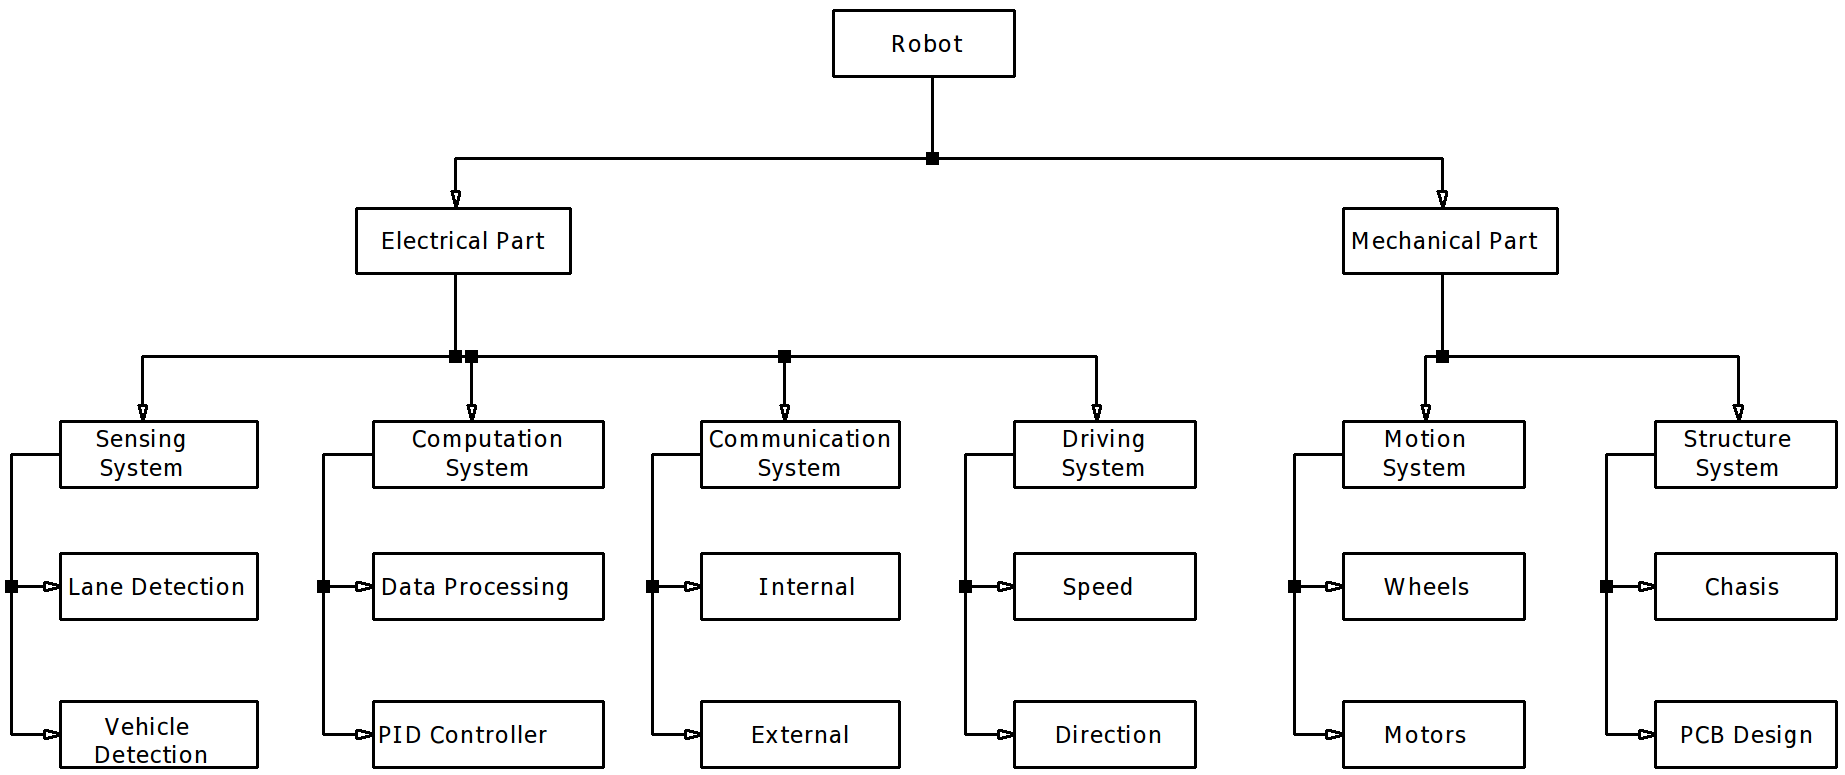
\includegraphics[width=\textwidth,center]{images/system}
		\caption{Organization of the Project}\label{fig:organization}
	\end{figure}
	
	
	
	
	V-Model is a very popular tool for system engineers to plan their projects. To ease the project tracking process, the V-Model was constructed by the DUAYENLER. The overall look of the V-Model can be seen at \textit{Figure~\ref{fig:vmodel}}. This section includes the explanation, requirements, test procedures and test results for the subsystems. In this section, the requirement for the systems and subsystems will be given. Moreover, the solution approaches for the subsystems will be explained in detail. Lastly, the solutions will be assessed by their performance according to their requirements. The test procedures and the discussion on the test results will be discussed in the preceding sections.
	
	\begin{figure}[h]
		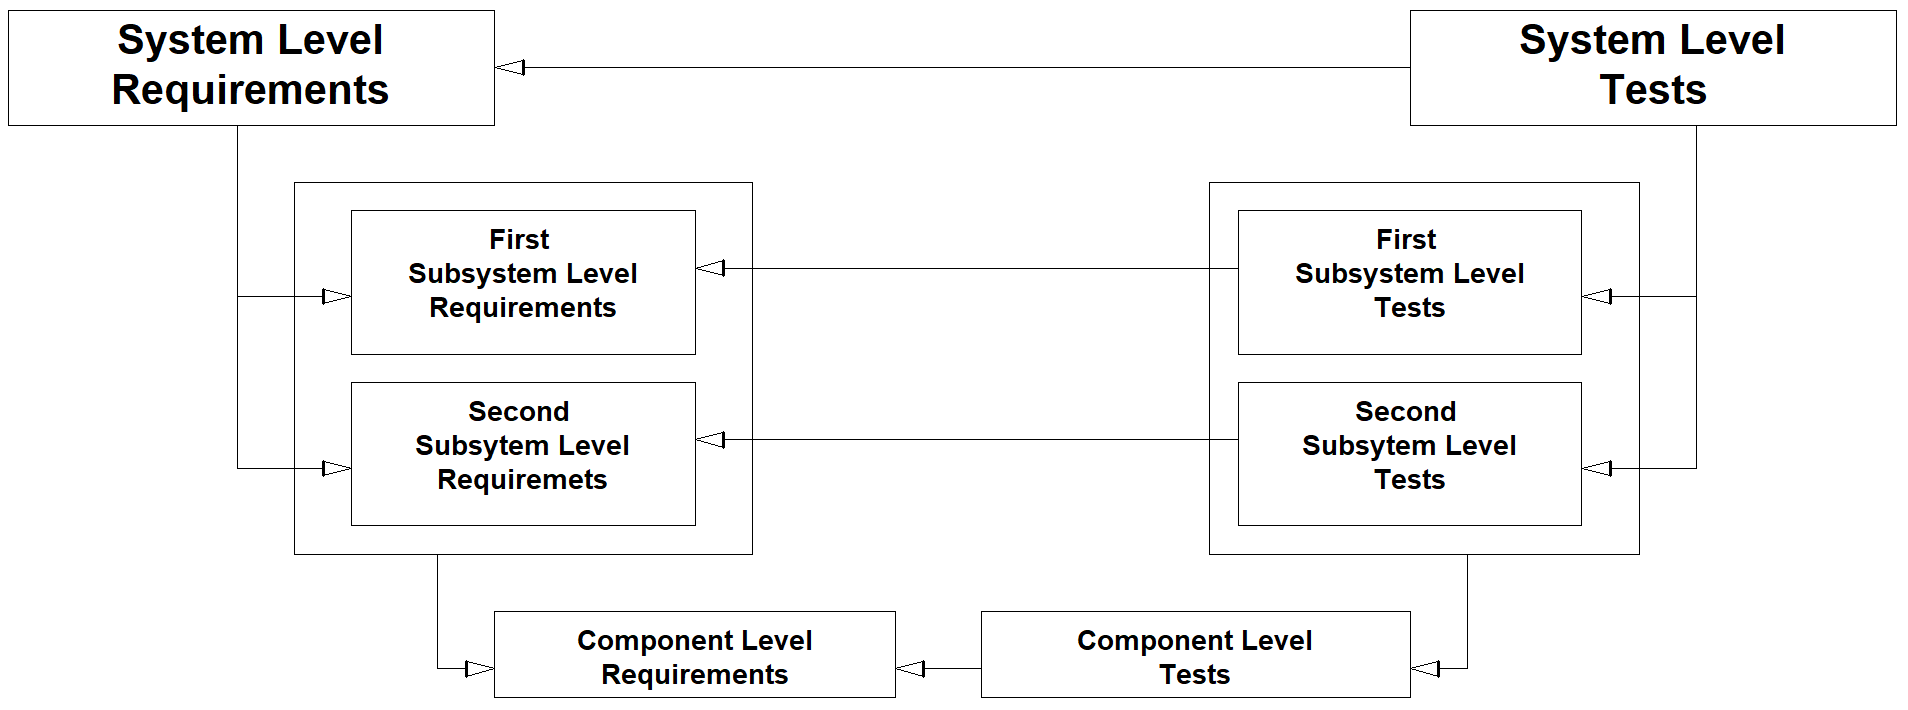
\includegraphics[width=\textwidth,center]{images/vModels/vmodel}
		\caption{V-Model}\label{fig:vmodel}
	\end{figure}
			
	%%%%%%%%%%%%%%%%%%%%%%%%%%%%%

Are they done?
\todo{justifications for requirements}\todo{Compliance with Reqs}
		
		
				
		
	%%%%%%%%%%%%%%%%%%%%%%%%%%%
		\subsection{Sensing System}
	
				This system is responsible for interpreting data from the environment. And the requirements for this system are as follows;
			\begin{enumerate}
		\item The system should detect the sides of the road.
		\item The system should not be effected from external disturbances.
		\item The system should detect the opponent vehicle.
				\end{enumerate}	
				The system has two subsystems namely, 
				
			\begin{enumerate}
				\item \textbf{Lane Detection Subsystem} which is responsible for detecting sides of the path as its name suggests
				\item \textbf{Vehicle Detection Subsystem} which is responsible for detecting opponent vehicle if it is close to the vehicle more than 5 cm
			\end{enumerate}
	
	
		\subsubsection{Lane Detection Subsystem}\label{sec:LaneDetectionSubsystem}

			\begin{enumerate}
			\item {Requirements for the Solution}

				
		
		
			
			\begin{enumerate}
				\item The subsystem should be able to detect only the shades of green color
				\item The subsystem should be able to detect edges in the camera frame in any light condition

			\end{enumerate}
			
		
			
			\begin{figure}[h]
			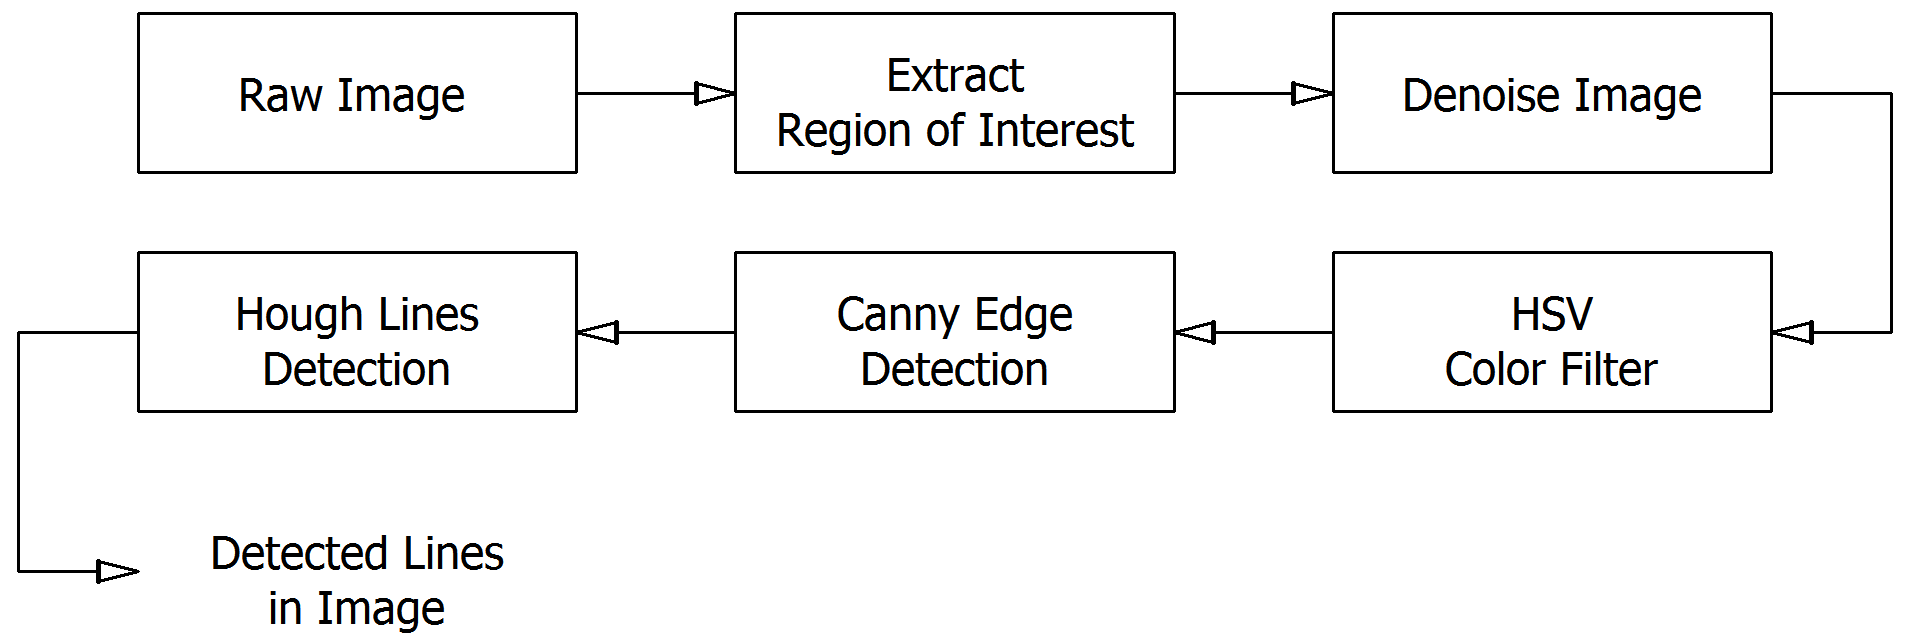
\includegraphics[width=0.93\textwidth,center]{images/vModels/laneDetection_subsystem}
			\caption{Block Diagram of the Lane Detection Subsystem}\label{fig:lane_detection_subsystem}
		\end{figure}
		
			
			
			\item {Solution for the Subsystem}
			
			The task of the subsystem is to detect the lane lines. The tool utilized to realize the task is OpenCV libraries together with developed pipelined algorithm.
			 The input to this subsystem is provided by Raspberry Pi camera mounted on top of the vehicle. The proposed solution first masks out a region of interest (ROI) of $480x250 px$. The masking eliminates the process of excessive data and increases the process speed of the pipeline. The explanations and visual of the ROI is provided in \textit{Section~\ref{sect:dataProcessingSubsystem}, Figure~\ref{fig:camera_vision_explained}}. Then, the target color green is filtered by applying Gaussian denoise (with zero mean) and HSV filters. The lower bound for HSV filter is [H=60, S=120, V=106] and the upper bound is [H=82, S=255, V=245]. This process colors the pixels that are in the green threshold to white and the rest to black. Next, the edges are detected by Canny edge detector. As edges are found, the pixels that may constitute a line are found by Hough line detector. The resulting output is an array of coordinates in the form of $[x_1, y_1, x_2, y_2]$ where $(x_1, y_1)$ is the starting point of the line and $(x_2, y_2)$ is the end point of the line. The found coordinate array is passed to Data Processing Subsystem. The block diagram of the subsystem is given in \textit{Figure~\ref{fig:lane_detection_subsystem}}.
		
			
			\item {Discussions on the Solution}
			
			The main structure of the proposed solution has not changed since Conceptual Design Report. An addition to process pipeline is extracting a ROI. This is done to both improve the performance and remove possible distractions that are present in the image. A point to note in this algorithm is Hough line detector. It is a probabilistic function, meaning that even if the captured frame is the same as previous frame, the found line coordinates may differentiate a bit. However, this is not a big issue. One weak point was the lane detection under extreme lighting conditions. The filter is adjusted to be able to detect in bright lighting conditions but dark lighting is problematic. To solve this issue, the team decided to place LED strips to front bumper of the vehicle.
			
		\end{enumerate}
	
	\subsubsection{Vehicle Detection Subsystem}
	
		
			\begin{enumerate}
			
			\item {Requirements for the Solution}
		
			\begin{enumerate}
				\item The subsystem should detect the opponent to be caught with in a 5 cm 
				\item The subsystem should detect the chasing opponent if it reaches from back with in a 5 cm 
				\item The subsystem should trigger the handshake protocol 
			\end{enumerate}
			
			\item {Solution for the Subsystem}
			
			The subsystem is the first step of safely competing with an opponent in a racing path. This subsystem uses two time of flight distance sensor which is enhanced IR sensor. One at the back of the vehicle responsible for detecting the chasing opponent and one at the front of the vehicle responsible for detecting the chased opponent. The subsystem produces positive output if the chasing vehicle or chased vehicle is within a range of 5 cm from the vehicle. Since the sensor reading is performed using Raspberry Pi, the required trigger for handshake protocol can be easily accessed by the external communication subsystem.
			
			\item {Discussions on the Solution}
			
			The proposed method is not entirely different than the one presented in Conceptual Design Report.  The only difference is the devices reading the sensors. In Conceptual Design Report, sensors were connected to Arduino. However, the team decided that it is problematic. For example, in the case of sensor readings from Arduino, when opponent is close, Arduino reads the sensor, sends it to trigger handshake, then Pi sends/receives TCP messages, then sends Arduino to stop the motors. On the other hand, reading sensors from Pi simplifies and accelerates the work by eliminating the step to send sensor reading. Also, since Raspberry Pi is a general-purpose computer, it can handle with complex tasks easily, while Arduino cannot. Therefore, sensors are moved from Arduino to Raspberry Pi.
			
		\end{enumerate}
	
	
	
	
	
			
	%%%%%%%%%%%%%%%%%%%%%%%%%%%	
		
		\subsection{Computation System}
		
		
		
			This system is responsible for computational works of the vehicle. The system mainly give meaning to data generated by the sensing system. And the requirements for this system are as follows; 
			
		\begin{enumerate}
			\item The system should	be able to produce middle line to follow
			\item The system should be able to control the robot
		\end{enumerate}	
			
			The system has two subsystems namely,
			
			\begin{enumerate}
				\item \textbf{Data Processing Subsystem} which is responsible for processing the output data of lane detection unit and produce data for PID control unit.
				\item \textbf{PID Controller Subsystem} which is responsible for controlling the motors of the vehicle.
			\end{enumerate}
			
		
		
		\subsubsection{Data Processing Subsystem}\label{sect:dataProcessingSubsystem}
		
		\begin{enumerate}
			\item {Requirements for the Solution}
			
				\begin{enumerate}
					\item The subsystem should be able to analyze data produced by sensing system
					\item The subsystem should be able to produce the angle information required by the controller subsystem
					\item The subsystem should be able to work on Raspberry Pi
					\item The subsystem should be able to process one frame at most in 100 milliseconds
					\item The subsystem should be able to tell differences between disturbances and lane
					\item The subsystem should be able to interpret the middle of the lane if both sides are present at the frame
				\end{enumerate}
				
			\item {Solution for the Subsystem}
			\begin{figure}[h]
				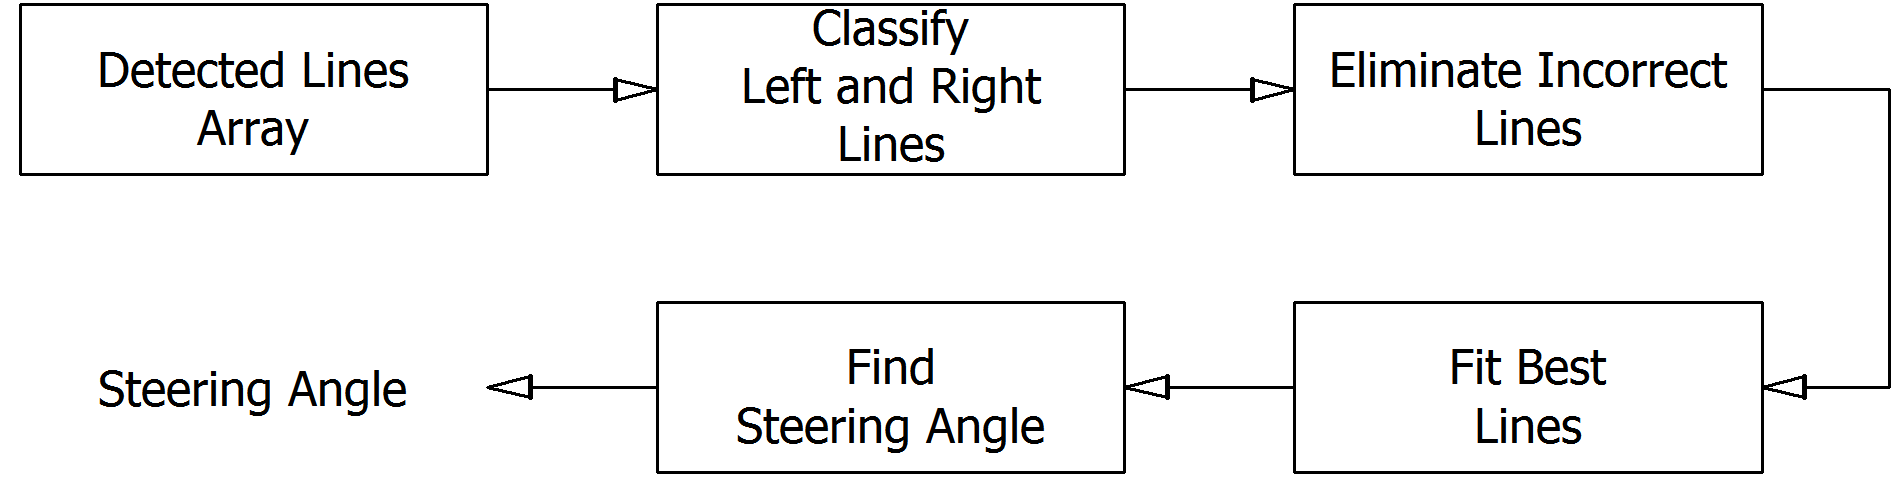
\includegraphics[width=0.93\textwidth,center]{images/vModels/dataProcessing_subsystem}
				\caption{Block Diagram of the Data Processing Subsystem}\label{fig:dataProcessing_subsystem}
			\end{figure}
			\begin{figure}[h]
				\centering
				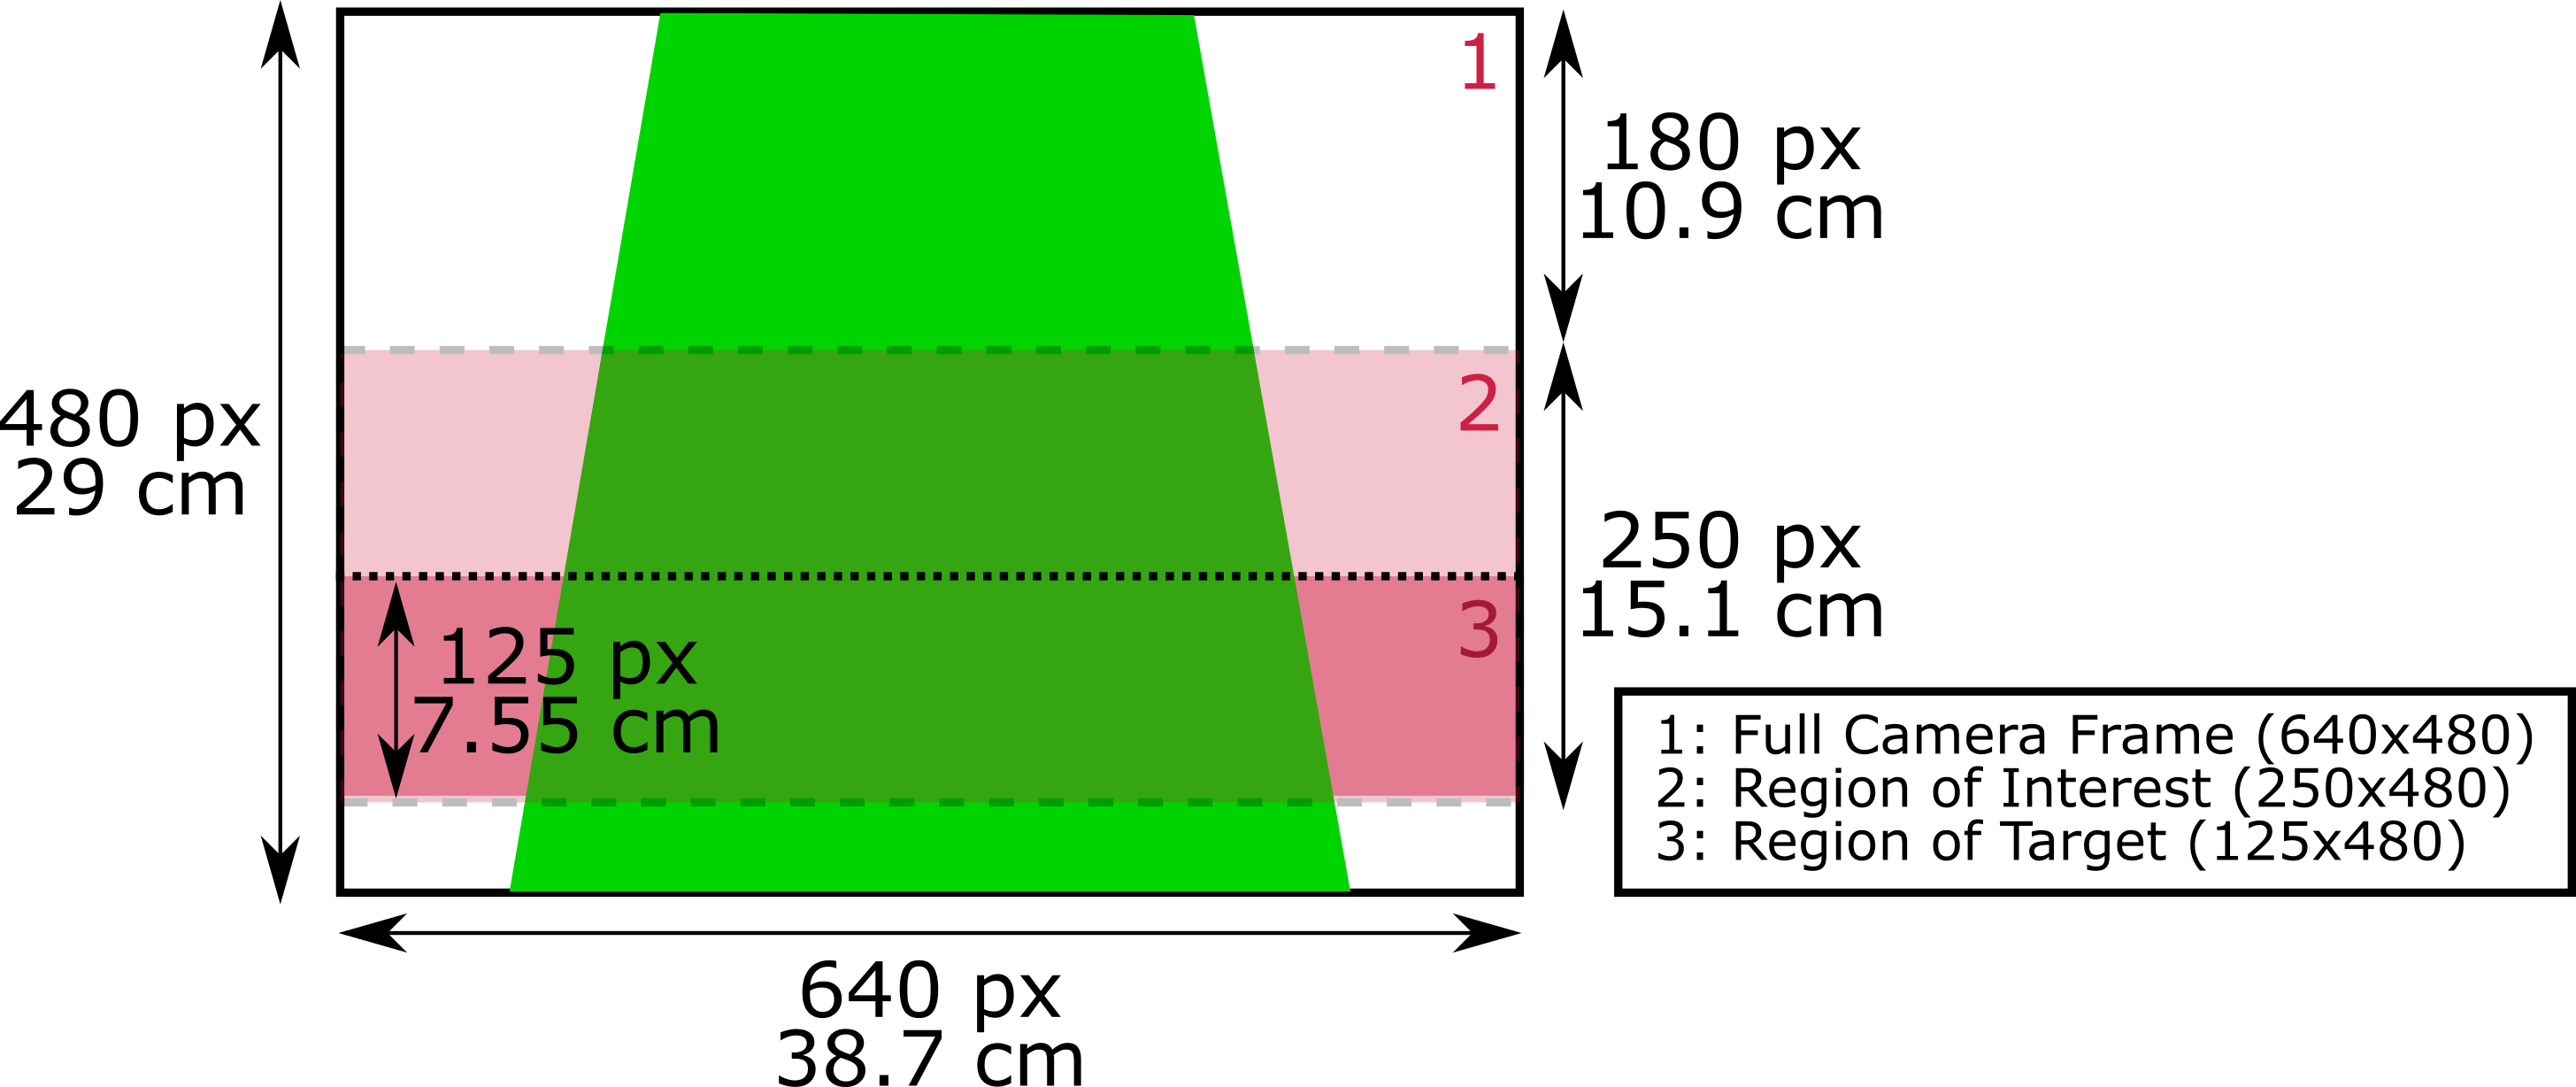
\includegraphics[width=0.93\textwidth]{images/camera_vision_explained}
				\caption{The Explanation of Frame Sections}\label{fig:camera_vision_explained}
			\end{figure}
		
			The task of this subsystem is to determine the steering angle of the vehicle so that the vehicle can steer to the target point. The input of the subsystem is the coordinate array produced by Lane Detection subsystem. The input is processed by a detailed algorithm and the output is steering angle. The processing is done by taking into consideration the reference frame. The reference frame is shown in \textit{Figure ~\ref{fig:camera_vision_explained}}. This figure summarizes the three frame sections that are used throughout this report. The Lane Detection subsystem extracted ROI out of full camera frame. The Data Processing subsystem processes the data of ROI but produces output for the Region of Target (ROT). The reason is, ROI is good to determine possible obstacles on the path but steering to a target point that is almost 15 cm away from the vehicle is not realistic.  For this reason ROI is not used for determining steering angle, instead ROT is used.
			
			There are four main steps to determine the steering angle.  The first step is to classify the lines as left and right. The second step is to eliminate the possible incorrect lines, if any. The third step is to fit the best lines through the left and right lines and reduce the total number of lines to two that are left and right lines. The last step is to find steering angle by connecting 320th horizontal pixel with the average end points of the lane lines. The block diagram of the subsystem is given in \textit{Figure~\ref{fig:dataProcessing_subsystem}}.
			
			Classifying a line is done in two steps. First, lines are divided into two whether they start from right or left of horizontal 320th pixel. Then, the center of both sets are found. Eventually, according to the average of both centers, lines are classified as left or right. This process is summarized in \textit{Algorithm~\ref{algo:classifyLines}}.
			
			
			\begin{algorithm}[b!]
				\caption{Classifying Lines as Left and Right}
				\label{algo:classifyLines}
				\DontPrintSemicolon
				
				%	\KwData{Testing set $x$}
				\For{All Lane Lines}    
				{ 
					\If{Starting Point $>$ 320}
					{
						Temporarily classify as right line 
					}
					\Else
					{
						Temporarily classify as left line 
					}
				}
				%	\KwData{Testing set $x$}
				r\_center = center of temporary right lines \;
				l\_center = center of temporary left lines \;
				
				lane\_center = (r\_center + l\_center)/2 \;
				
				\For{All Lane Lines}    
				{ 
					\If{Starting Point $>$ lane\_center}
					{
						Classify as right line 
					}
					\Else
					{
						Classify as left line 
					}
				}
			\end{algorithm}
			\begin{figure}[b!]
				\setlength{\unitlength}{\textwidth} 
				\centering
				\begin{subfigure}{.46\textwidth}
					\centering
					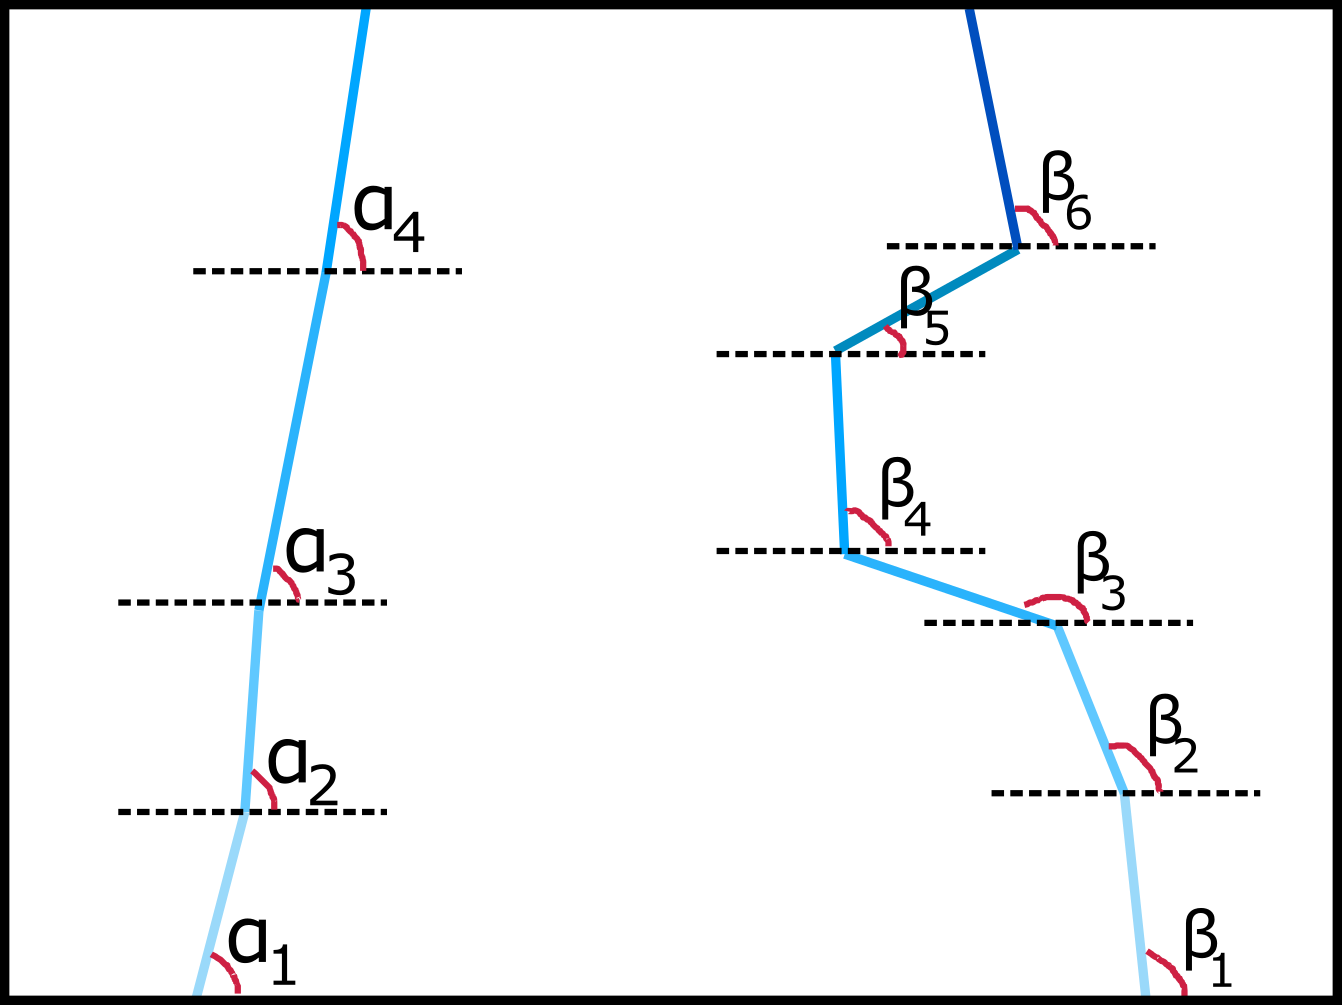
\includegraphics[width=0.44\unitlength]{images/dataP_explained1}
					\caption{\label{fig:dataP_explained1} Before Eliminating Incorrect Lines}
				\end{subfigure}%
				\begin{subfigure}{.46\textwidth}
					\centering
					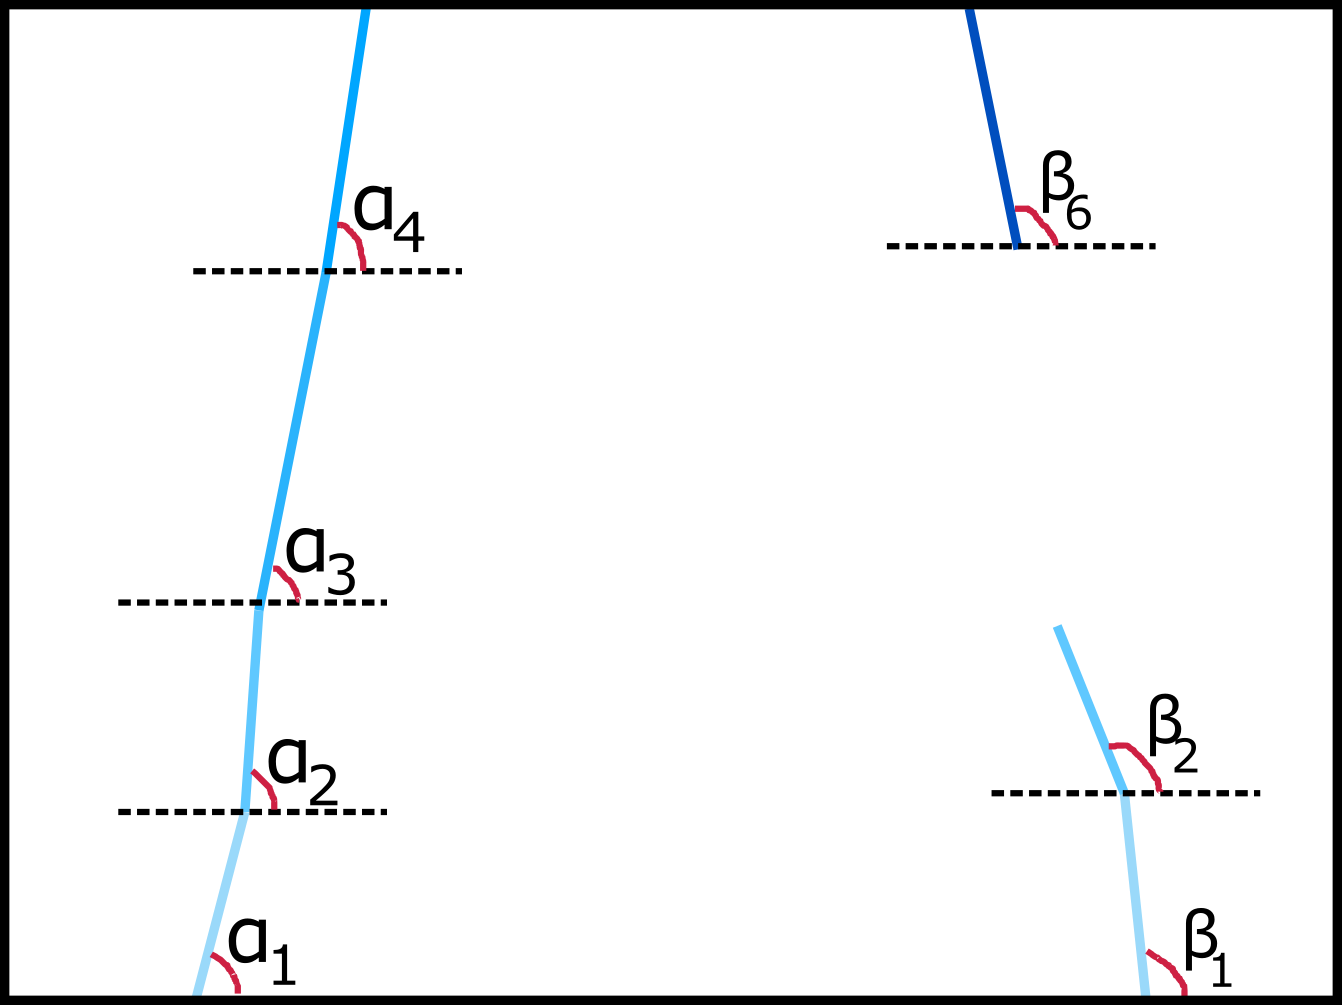
\includegraphics[width=0.44\unitlength]{images/dataP_explained2}
					\caption{\label{fig:dataP_explained2} After Eliminating Incorrect Lines}
				\end{subfigure}
				\caption{\label{fig:dataP_explained} A Sample Scenario on Eliminating Incorrect Lines}
			\end{figure}



	
	The next step is to determine whether there are disturbances on the lane lines or not. This is the most complex part of the Data Processing subsystem. Actually the correctness of the steering angle depends on how successful this step is realized. The idea behind this step is evaluating the slopes consecutive lines and assessing whether change in the slope is ordinary or abnormal. The \textit{Figure~\ref{fig:dataP_explained}} exemplifies a possible scenario. In this figure, the blue lines represent the detected lines in ROI whereas $\alpha$ and $\beta$ represent the slopes of the detected lines. Clearly, there are no disturbance on left lines since $\alpha$ values are similar to each other. However if $\beta$ values are observed, possibly there is an obstacle on right line covered by $\beta_3$, $\beta_4$ and $\beta_5$. This can be concluded by observing slope differences $(\beta_2 - \beta_3)$ and $(\beta_5 - \beta_6)$. To ignore this obstacle, it is enough to remove lines with slopes $\beta_3$, $\beta_4$ and $\beta_5$ as in \textit{Figure~\ref{fig:dataP_explained2}}. Even though the count of lines is decreased, elimination of incorrect lines are realized and the best line fit will be more correct. Another scenario is shown in \textit{Figure~\ref{fig:dataP_explainedBroken}}. Again the shown lines are the ones in ROI. In this scenario, left line has no problems. Right lines, however, a bit problematic. The problem is revealed when  $(\beta_3 - \beta_4)$ is observed. To determine whether  $(\beta_1, \beta_2, \beta_3)$ or $(\beta_4, \beta_5)$ is the correct set of lines, left lines are observed and the set which is more symmetric to left lines are selected as right lines. The resulting correction is shown in \textit{Figure~\ref{fig:dataP_explained4}}.	This is the basic idea behind eliminating incorrect lines in Data Processing subsystem. This idea is generalized by considering other possible obstacle types and shapes. The generalized idea is complicated and would take too long to present here. The summarized idea is presented in \textit{Algorithm~\ref{algo:eliminateLines}}.
	\begin{figure}[b!]
	\setlength{\unitlength}{\textwidth} 
	\centering
	\begin{subfigure}{.46\textwidth}
		\centering
		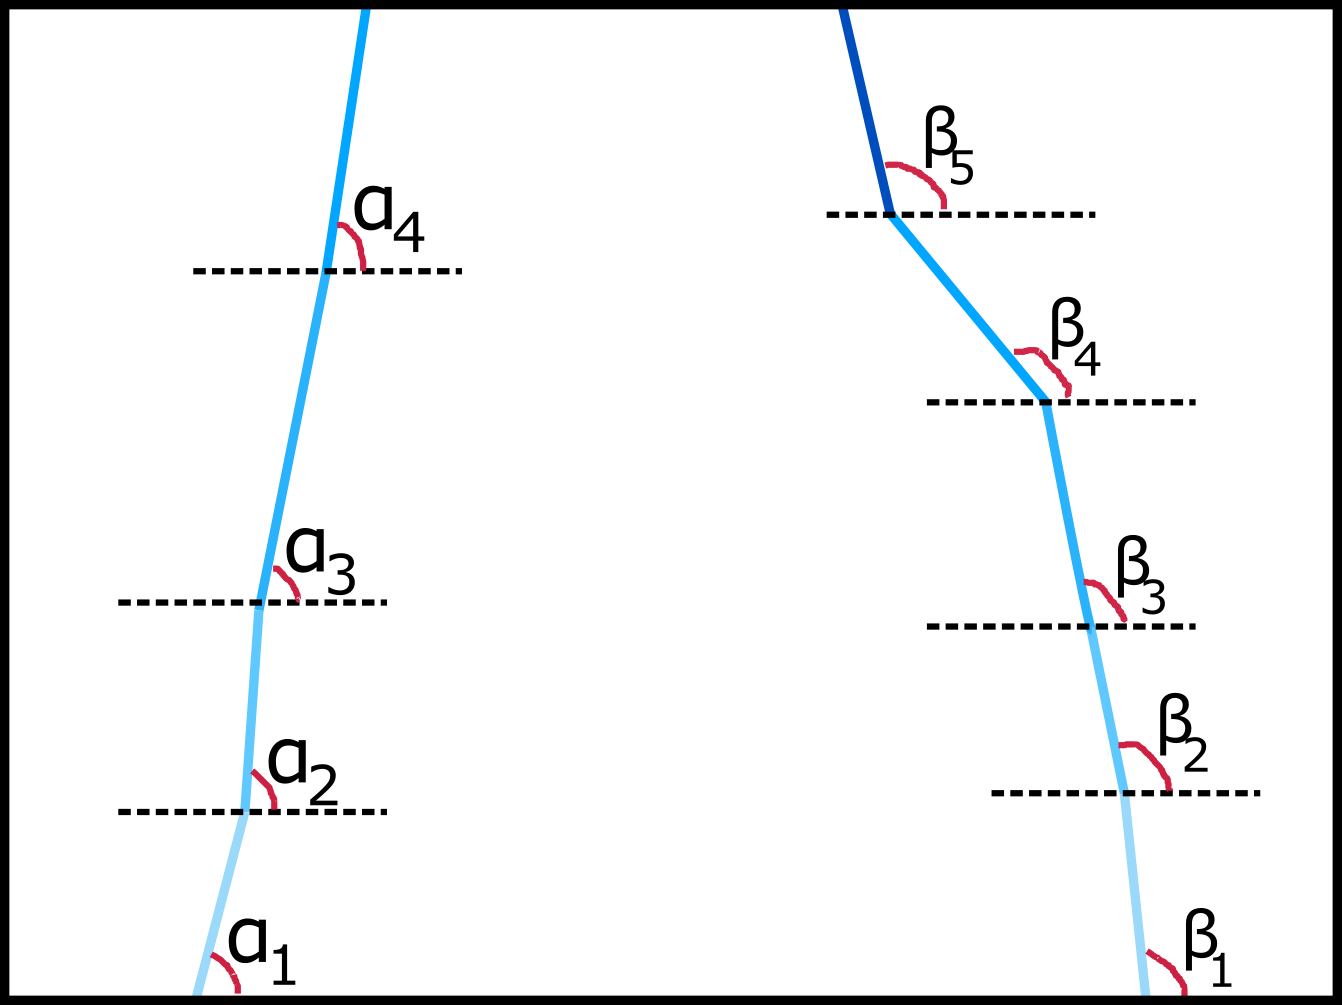
\includegraphics[width=0.44\unitlength]{images/dataP_explained3}
		\caption{\label{fig:dataP_explained3} Before Eliminating Incorrect Lines}
	\end{subfigure}%
	\begin{subfigure}{.46\textwidth}
		\centering
		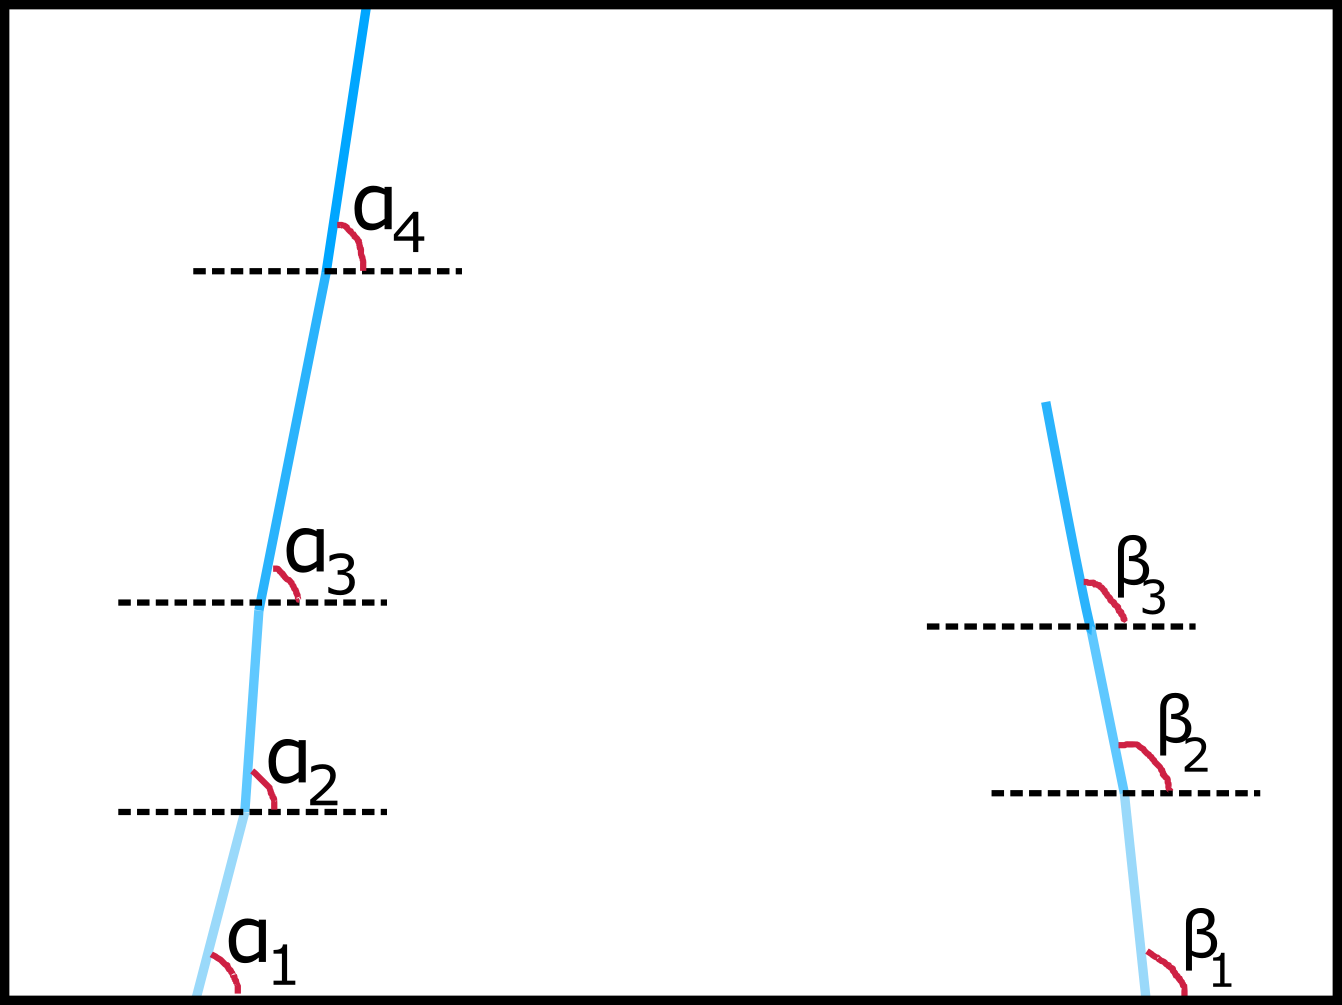
\includegraphics[width=0.44\unitlength]{images/dataP_explained4}
		\caption{\label{fig:dataP_explained4} After Eliminating Incorrect Lines}
	\end{subfigure}
	\caption{\label{fig:dataP_explainedBroken} Another Scenario on Eliminating Incorrect Lines}
\end{figure}
\begin{algorithm}[b!]
	\caption{Line Elimination Algorithm}
	\label{algo:eliminateLines}
	\DontPrintSemicolon
	
	array[n] lines \;
	array[n] line\_slope\_angles \;
	array[n-1] slope\_angle\_differences \;
	
	slopeAngle\_threshold \;
	slopeAngle\_difference\_threshold \;
	
	%	\KwData{Testing set $x$}
	\For{slope\_angle\_differences}
	{ 
		\If{$k$th item $>$ slopeAngle\_difference\_threshold}
		{
			// Check $k$th and $(k+1)$th items in line\_slope\_angles array \;
			\If{$k$th item in line\_slope\_angles array $>$	slopeAngle\_threshold}
			{
				Mark index $k$ in lines array problematic
			}	
			\ElseIf{$(k+1)$th item in line\_slope\_angles array $>$	slopeAngle\_threshold}
			{
				Mark index $(k+1)$ in lines array problematic
			}	
		}
	}
	Delete the lines between problematic indexes \;
	
\end{algorithm}



	The third step is to fit best lines through the remaining lines. This is realized by using built-in Least-Squares method. As a result of this step, the number of lines is dropped to two as left line and right line.
	
	The last step is to find the steering angle. The target point is determined as the average of the middle points left and right lines. So the target point is always in the form of $(x_{avg}, 305)$. The y-coordinate is found by simple math (referencing from \textit{Figure~\ref{fig:camera_vision_explained}}) $480px-50px-125px$. The current point of the vehicle is always $(320,480)$. So the line connecting two points to each other constitutes the track path and the $arctan$ of the slope gives the steering angle. Steering angle is in the $[-90,90]$ range where negative values indicate to turn left and positive values indicate to turn right. This output is sent to PID Controller subsystem.
			
		\item {Discussions on the Solution}
		
	The proposed algorithm is different from the one presented in Conceptual Design Report. The reason is that the old algorithm didn't have any obstacle rejection	feature and it had problems in determining steering angle. For this reason, new algorithm is developed from scratch. The proposed algorithm works nice as test results are discussed in \textit{Section~\ref{sec:DataProcessingSubsystemTests}}. The obstacles are most of the time are detected and ignored. One weak point is that, the algorithm may not be able to ignore some obstacles in certain inclinations. That is, as algorithm is based on slope evaluation, certain obstacle placements may fool the algorithm.
			
		\end{enumerate}
	
		
		
		\subsubsection{PID Controller Subsystem}
		
			\begin{enumerate}
				\item {Requirements for the Solution}
			
				\begin{enumerate}
						\item The subsystem should be able to control the motors
						\item The subsystem should be able to react the external disturbances
					\end{enumerate} 
					
				\item {Solution for the Subsystem}
				
	\textit{PID Controller Subsection} ,as its name suggests, is the main controller element of the vehicle that is responsible for controlling the lateral movement of the vehicle. As the achieved purpose is to stay in the middle of the lane, this subsystem creates a PWM differences between motors in order to rotate the vehicle via differential drive. 
	
	For that purpose, the \textit{Data Processing Subsystem} produces the necessary feedback elements for this subsystem. For the control purpose, in ideal circumstances data processing unit determines eight main point on its vision to create processed variables as in \textit{Figure~\ref{fig:controlled-vars}}. These can be explained namely as;
	\begin{itemize}
		\item \textbf{A1 \& A2:} Beginning and end points of left line at ROT (Region of Target).
		\item \textbf{B1 \& B2:} Beginning and end points of right line at ROT.	
		\item \textbf{Image Center Back (ICB):} Beginning point of our heading line in ROT.
		\item \textbf{Image Center Front (ICF):} End point of our heading line in ROT.  
		\item \textbf{Lane Center Back (LCB):} The middle point of the lane at the starting of the ROT. Can be found by averaging $A1$ $\&$ $B1$.
		\item \textbf{Lane Center Front (LCF):} The middle point of the lane at the end of the ROT. Can be found by averaging $A2$ $\&$ $B2$.
	\end{itemize}	   
				
				
				
				%%%%%%%%%%%%%%%%%%%%%%%%%%%
				
				%\begin{figure}[h]
				%	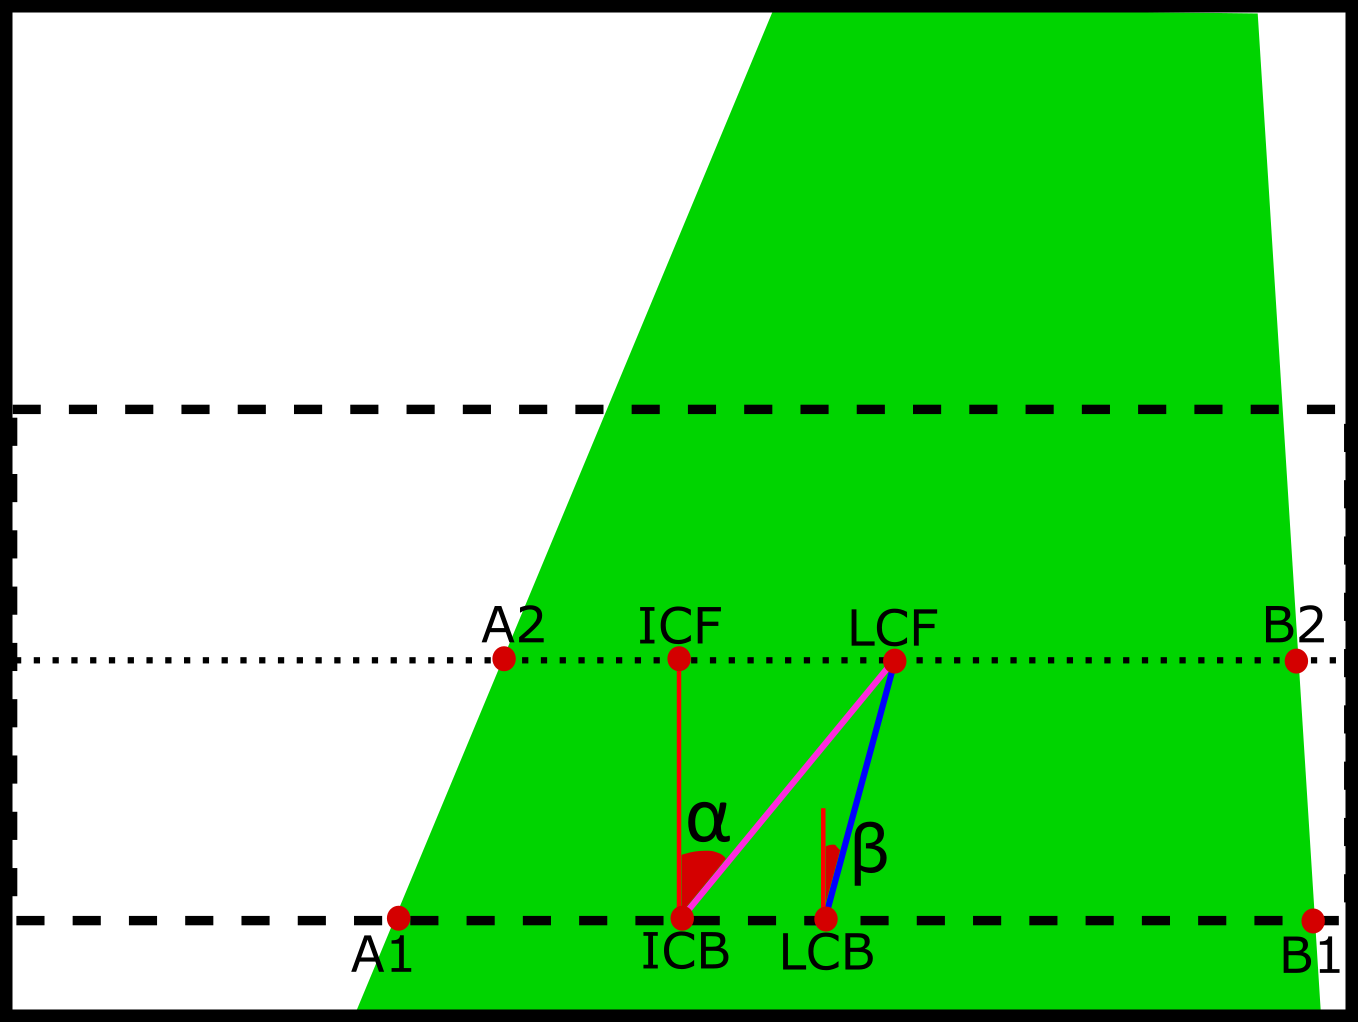
\includegraphics[width=0.75\textwidth,center]{images/ang_cont}
				%	\caption{System organization of the project}\label{fig:organization}
				%\end{figure}
				
				
				\begin{figure}[H]
					\setlength{\unitlength}{\textwidth} 
					\centering
					\begin{subfigure}{.46\textwidth}
	  					\centering
	  					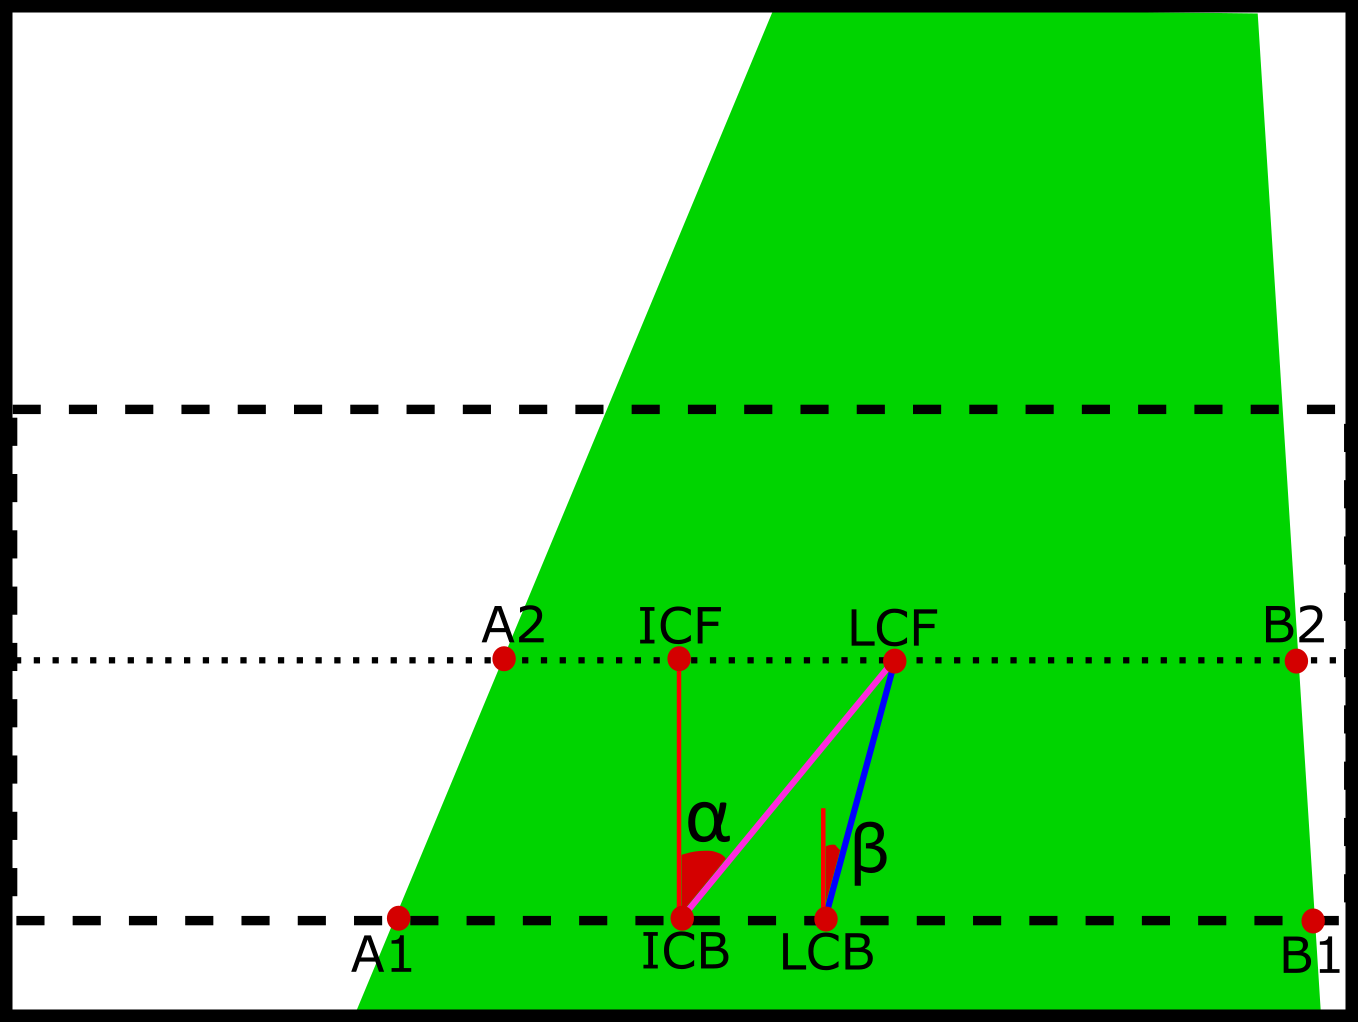
\includegraphics[width=0.45\unitlength]{images/ang_cont}
	  					\caption{\label{fig:ang-cont} Controllable Angle Variables }
				\end{subfigure}%
				\begin{subfigure}{.46\textwidth}
	  				\centering
					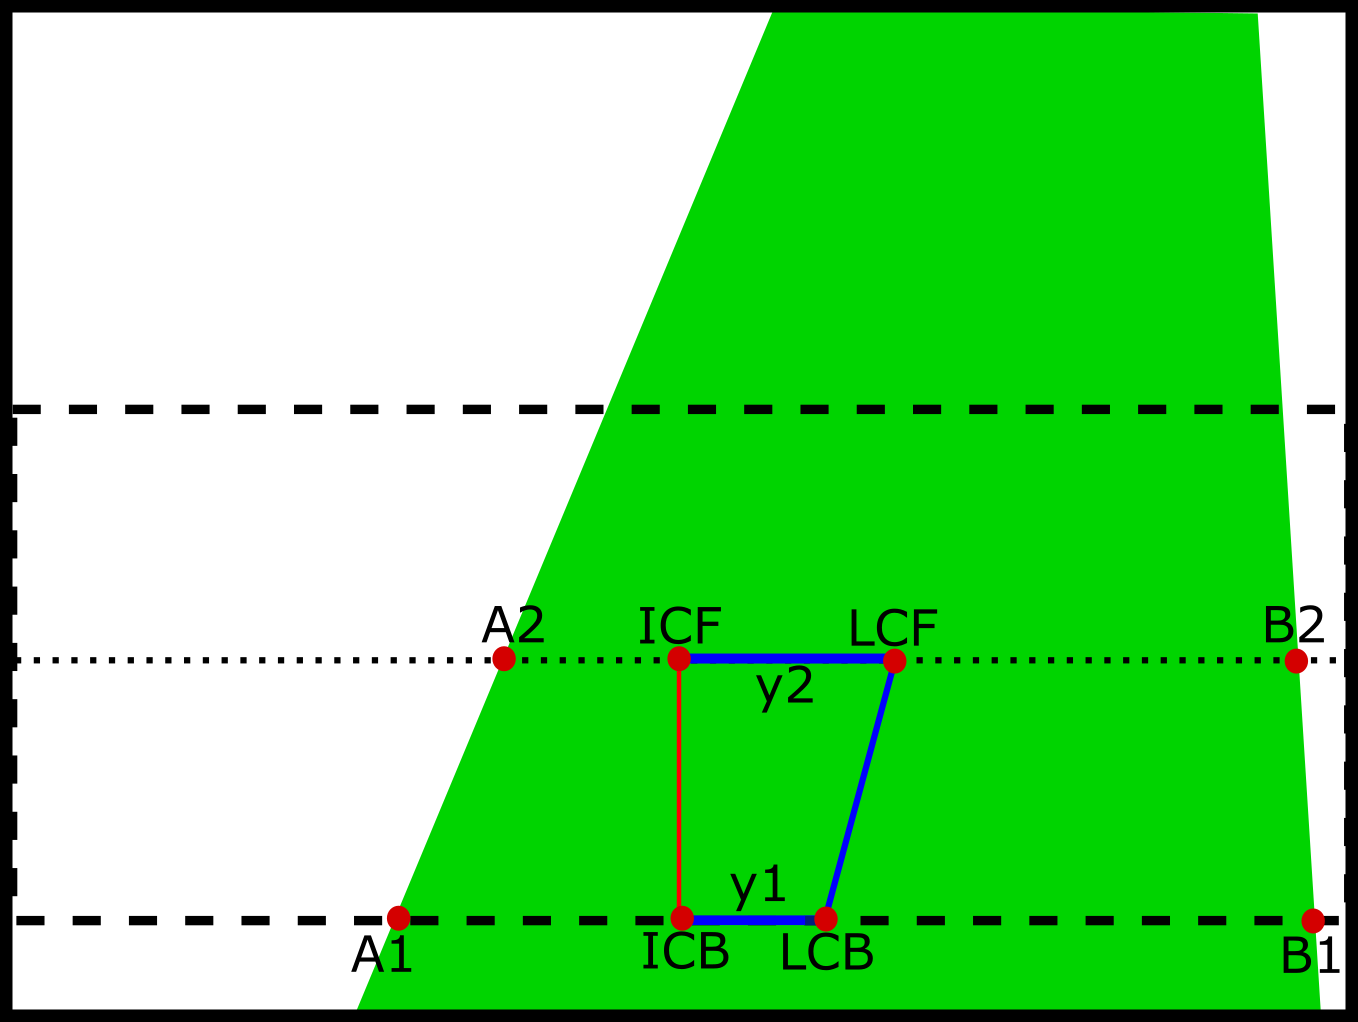
\includegraphics[width=0.45\unitlength]{images/dist_cont}
	  				\caption{\label{fig:dist-cont} Controllable Distance Variables}
				\end{subfigure}
				\caption{\label{fig:controlled-vars} Controlled Variables of the System }
			\end{figure}
	
			%%%%%%%%%%%%%%%%%%%%%%%%%%%
				
	By utilizing these points and their coordinates, the data processing can produce four main variables that can bee used for PID controller and speed subsystems. These are;
	
	\begin{itemize}
		\item \textbf{$\alpha$:} The angle between the current direction of the vehicle and the direction the vehicle should follow in order to arrive at point \textbf{LCF}. It is a main controlled variable for lateral position control with angle variable.
		
		\item \textbf{$\beta$:} The angle of the line that connects the points \textbf{LCB} and \textbf{LCF}. It represents the angle of the lane, and it can be used for longitudinal movement control in speed subsystem.
		
		\item \textbf{y1:} The instantaneous distance error of the vehicle from the center line. It can be calculated by subtracting the x-coordinate of \textbf{LCB} from the x-coordinate of \textbf{ICB}. Due to delays in the system, it is not fed to controller. However, it is a quite useful variable for observing the system.  
		
		\item \textbf{y2:} The expected distance error of the vehicle from the center line at the end of ROT. It can be calculated by subtracting the x-coordinate of \textbf{LCF} from the x-coordinate of \textbf{ICF}. This results in a distance in a scale of pixels, to convert this to a distance in centimeter, the error can be multiplies by a constant. It is a main controlled variable for lateral position control with distance variable.
	
	
	\end{itemize}	 			

	
	\subsubsection*{Modelling the Plant}
	
	Modelling a plant is a good practice in controller design applications, however, in our case the model for the vehicle is unstable, thus applying a bump test as in \textit{Figure~\ref{fig:bump2}} results with a exponentially increasing processed data 'y2'. Thus, in this project, our aim is to apply bump test to closed loop system as in \textit{Figure~\ref{fig:bump1}} with a known P-controller. An approximate plant model from there can be found as follows;
	
	$$ T(s)=\frac{G_c(s)G_p(s)}{1+G_c(s)G_p(s)} $$
	
	If the overall step response can be modelled resulting with $T(s)$
	
	$$\boxed{ G_p(s)=\frac{T(s)}{G_c(s)-T(s)G_c(s)} }$$ 
	
	Using this plant model, parameters for PID controller can be designed using \textit{Matlab Simulink}.
		
		\begin{figure}[h]
			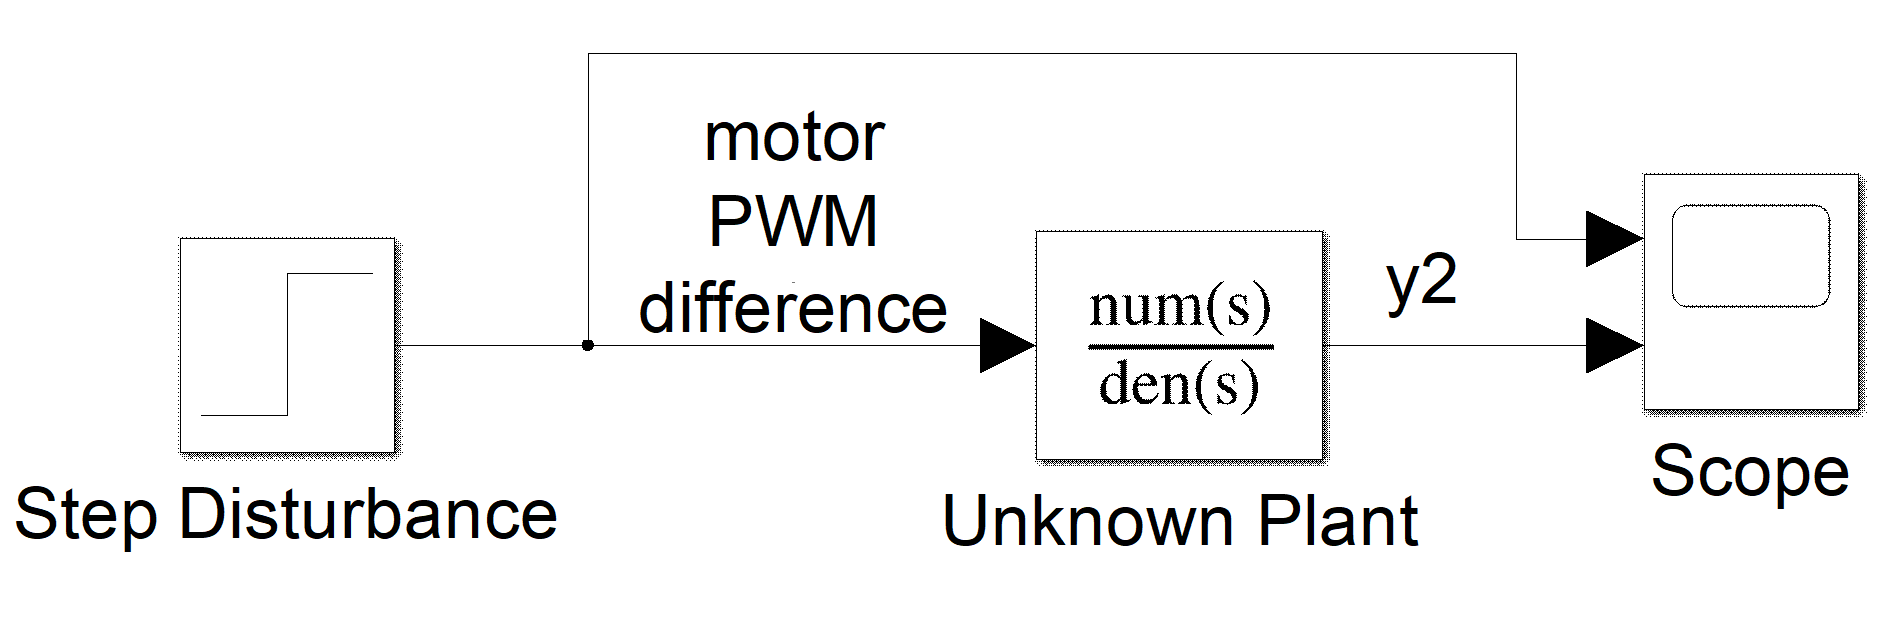
\includegraphics[width=0.75\textwidth,center]{images/simulink/modelling2}
			\caption{Bump Test for the Unknown Plant \label{fig:bump2} }
		\end{figure}

		\begin{figure}[h]
			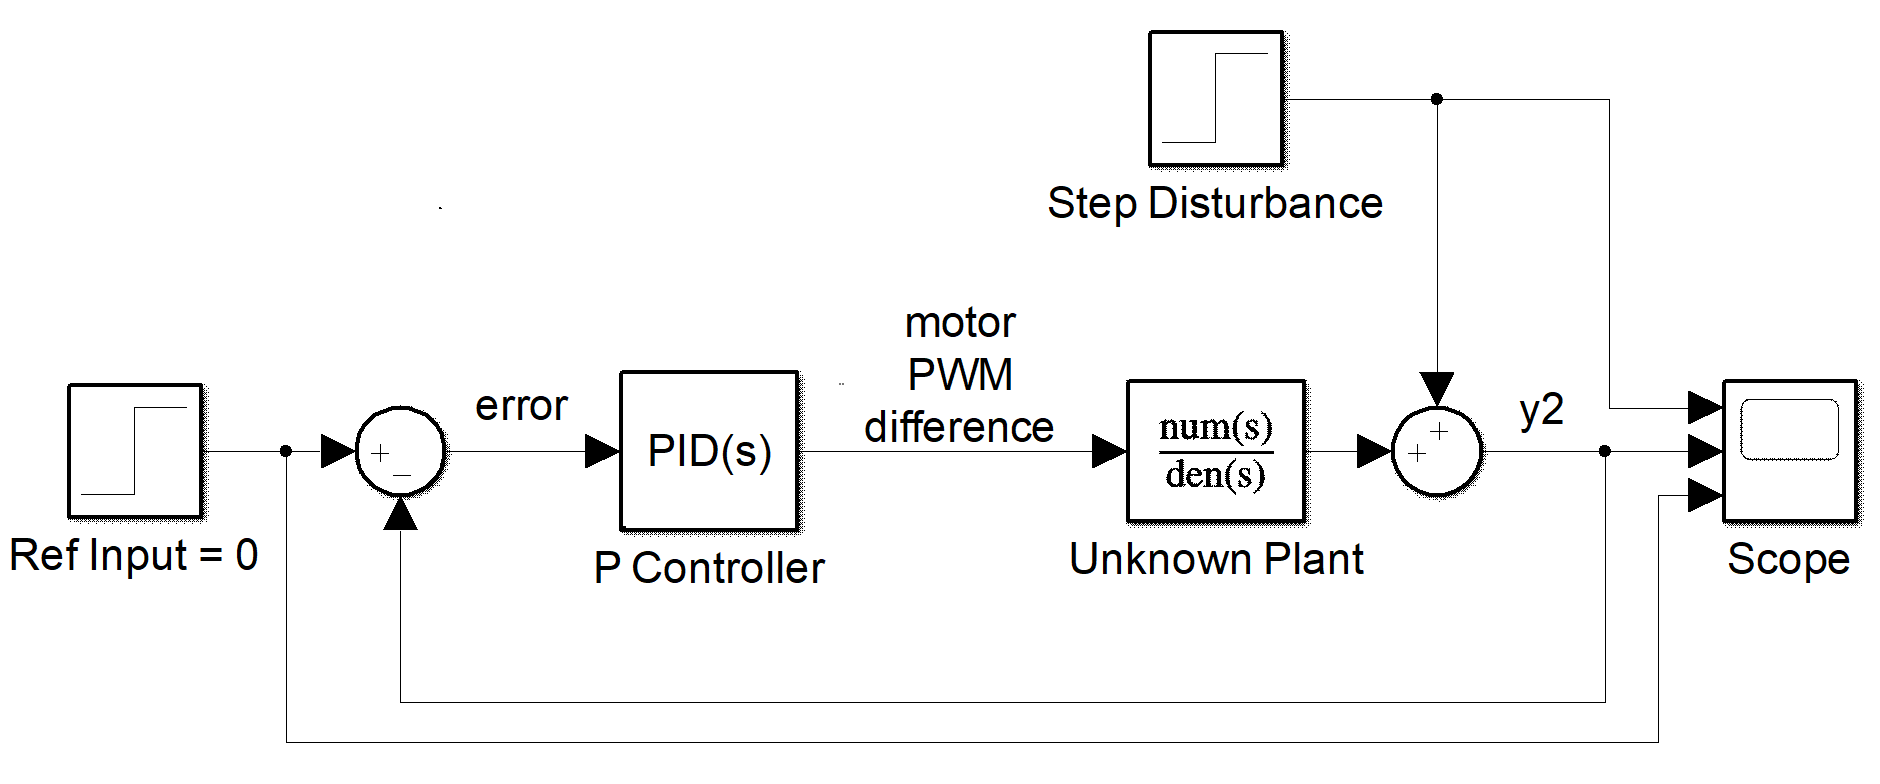
\includegraphics[width=1\textwidth,center]{images/simulink/modelling1}
			\caption{Bump Test for the Closed Loop System \label{fig:bump1} }
		\end{figure}
		
	\subsubsection*{Design \& Implementation of the Controller }
	
	General PID controller can be expressed in \textit{Laplace} domain as
	
	$$ G_c(s)=K_c(1+\frac{1}{\tau_I s}+\tau_d s )$$ 
	
	This is a transfer function that accepts the error signal as its input as in \textit{Figure~\ref{fig:bump1}}. Since the reference input is always zero for our case, in other words, it is desired that the variables $\alpha $ and $ y2 $ is equal to zero for all time instants. Therefore, for our case, the error is equal to the negative version of controlled variable.
	
	For implementation, the angle variable $\alpha$ and the distance variable $y2$ can be fed to the Arduino board by the help of \textit{Internal Communication Subsystem}. The implementation is a Arduino code written to produce a PWM-offset value from the error data. The PID parameters found using the simulink can be inserted in this code easily.
		

				
				\item {Discussions on the Solution}
	
	Although the basic idea behind control algorithm is same as the algorithm it has been significantly improved after the conceptual design report to compensate our needs and handle the resources the Data Processing Subsystem have. The \textbf{PID Controller Subsystem Test} explained in \textbf{Section~\ref{test_sec}} were not fully executed due to lack of incompleteness of the overall design. However, the test that were conducted for the bump tests were promising.	
			
			\end{enumerate}
		
		
			
		
		
			
	%%%%%%%%%%%%%%%%%%%%%%%%%%%	
			
		\subsection{Communication System}
			
		This systems is responsible for all communication responsibility of the system. It is one of the most crucial systems of this project since it is responsible for safe communication between subsystems with each other. It is also responsible for communication with other vehicles.	And the requirements for this system are as follows;		
		
			\begin{enumerate}
				\item The subsystem should ensure safe internal communication
				\item The subsystem should ensure safe external communication
			\end{enumerate}	
		
		
		The system has two subsystems namely, 	,
		
			\begin{enumerate}
				\item \textbf{Internal Communication Subsystem} which is responsible for communication inside the vehicle mainly the communication between Raspberry Pi and Arduino.						
				\item \textbf{External Communication Subsystem} which is responsible for the communication of the vehicle with the outside world mainly with the opponents.
			\end{enumerate}		
			
			
		\subsubsection{Internal Communication Subsystem}
		
			\begin{enumerate}
				\item {Requirements for the Solution}
				
				\begin{enumerate}
					\item The microcontrollers should be able to communicate with each other via serial communication
					\item The internal communication speed should be compatible with the processing speed of the lane detection subsystem  
				\end{enumerate}
			
				\item {Solution for the Subsystem}
				
				This subsystem covers the communication of the components inside vehicle. Currently, Raspberry Pi and Arduino are two components that requires communication. To prevent the large amount of cable connection, a serial communication protocol is implemented. 
		\begin{lstlisting}[language=Python,float=h!,numbers=left,frame=single,caption=Serial object decleration in Python,label=sc:serial_python, captionpos=b ] 
import serial
ar=serial.Serial("/dev/ttyUSB0",9600)
		\end{lstlisting}
		 \begin{lstlisting}[language=C,float=h!,numbers=left,frame=single,caption=Serial communication setup in C,label=sc:serial_c, captionpos=b ] 
#include "./arduinoModule/rs232.h"
int cport_nr = 24; /* /dev/ttyUSB0 */
int bdrate = 9600; /* 9600 baud */
char mode[] = { '8', 'N', '1', 0 }; // 8 data bits, no parity, 1 stop bit
char str_send[2][BUF_SIZE]; // send data buffer
unsigned char str_recv[BUF_SIZE]; // recv data buffer
RS232_OpenComport(cport_nr, bdrate, mode);
		\end{lstlisting}
	
	There are several serial communication protocols that can be used to maintain the connection such as SPI, I2C. However, the first choice is to use USB serial port of the Arduino. Since RPi is practically a computer, it can recognize Arduino as a device using a serial port such as \lstinline|/ttyUSB0| in case of a Linux based OS. When recognized, RPi can send any piece of strings to the Arduino via USB cable. The process of communication is as follows:
	\begin{enumerate}
		\item Arduino should be connected to the Pi. \vspace{-0.2cm}
		\item Using Arduino IDE or any other method such as listing serial ports and checking for Arduino and so on, the serial port name should be detected \vspace{-0.2cm}
		\item Baud rates of two sides should be the same. 9600 is generally enough but if needed, it can be incremented to satisfy fast communication \vspace{-0.2cm}
		\item On Arduino side, \texttt{Serial.begin(9600)} command should be executed and serial port should be read repeatedly to capture the incoming data \vspace{-0.2cm}
		\item On Pi side, using any language C++ or Python, messages to serial port can be send 
	\end{enumerate}
	
	There are minor differences when implementing the code in Python, C++  and C. Python is the most practical one:\\
	
	Python has a library called serial by which any type of data can be send through serial ports. Script \ref{sc:serial_python} is used to declare a serial object. Then using \texttt{ar.write("some string \textbackslash r".encode())}, the string "some string" can be send to Arduino. Note that "\textbackslash r" carriage return character carries a high importance because it shows that a string is terminated and any other incoming data belongs to the new piece of string.   \\
	

	As alternatives, the implementation on C is also examined.	Sample codes to implement the same communication in C is in Script \ref{sc:serial_c}. Since it is a low level language, specification of buffer size and other parameters should be done in the code.\\

	%\lstinline[language=Arduino]|<SerialCommand.h>| 
	On Arduino  side, there are also several option that we can read the incoming data. Using \texttt{Serial.read()}  command is one of the simplest solutions. However, it contains some issues like conversion from string to integer and when to stop. Furthermore, the incoming data should be considered in character basis for the exact control.  
	
	\paragraph*{Alternative Solutions for Internal Communication Subsystem}
		The communication between Raspberry Pi and Arduino can be realized by the use of other peripheral protocols or libraries.\\
	
		There is a \texttt{SerialCommand.h} library for the Arduino which allows executing a function depending on the incoming string. Using \lstinline|.addCommand("str",func)| of the library any function can be associated with any string coming from serial port. Moreover, the functions can have argument. For example, let the string "PWMSET" be execute a function \lstinline|setpwm()| but the PWM value is required. If incoming string is of the form "PWMSET 150", using \lstinline|.next()| function of the library, the value 150 can be read and converted into integer and interpreted as the PWM value to be set.\\
		
		Another solution is to use I2C or SPI protocols to set communication between Arduino and Raspberry Pi. These options require simple wiring connections between the pins. A point to remark is being cautious to operating voltage levels of pins of Arduino and Raspberry Pi.\\
		
		Besides aforementioned alternatives, Wi-Fi communication can also be considered between Arduino and Raspberry Pi. This solution requires deployment of a Wi-Fi module on Arduino. Some hardware exists in market such as ESP8266 and EMW3165. This solution would require a Wi-Fi network in the medium which makes the solution less implementable.\\
		
		A last solution would be to remove Arduino from the system. This would require the handover of operations of Arduino to Raspberry Pi. The resulting system could be considered as a single board solution, that is, all relevant subsystems operate on Raspberry Pi. This option would cause heating problems on Raspberry Pi. A cooling mechanism should also be applicable in this case.
		
		Communication subsystem enables the robot to communicate with the opponent using the handshake protocol agreed on standard committee. According to the standard committee, Wi-Fi modules must be used to implement handshaking. Since Raspberry Pi was used in the project, there is no need to get a separate Wi-Fi module; the internal Wi-Fi module of the Raspberry Pi was used.
			
				\item {Discussions on the Solution}
				
			\end{enumerate}
			
			
	

	\subsubsection{External Communication Subsystem}	
	
		\begin{enumerate}
			\item {Requirements for the Solution}
			\begin{enumerate}
				\item The subsystem must be able to communicate with the opponent via P2P Wi-Fi protocol
				\item The subsystem must start race with a handshake mechanism
				\item Similarly, the subsystem must be able to trigger another handshake mechanism at the end of the race
				\item For the second handshaking, the subsystem must be able to get the sensor data from vehicle detection subsystem to send messages
			\end{enumerate}
			\item {Solution for the Subsystem}
			
		The main solution for this subsystem is setting the device as a P2P host. Sockets are used to send or receive messages.  Since the host can act as a server as well as a client, both socket functions are used to establish communication. The subsystem requires opponent ID from the user and sensor readings from the vehicle detection subsystem. It can initiate and terminate other subsystems.
		
		Firstly, the socket data structures are created in both server and client sides. In the beginning of the race, the peer acting as a server listens to the port 5000, which is specified in Standard Committee. Then, the connect() function is called in the client side, so that the request is sent. At the same time, server side acknowledges the request by means of accept() function. At this moment, client side also sends acknowledgement by default, hence race starts. The peers are connected during the race.
		
		The process for the finishing handshake also utilizes socket functions, but the process is a little bit different. For the win case, vehicle detection subsystem (front sensor) initiates the handshake. A catch message (ID00) is sent to the opponent. If acknowledgment is taken from the opponent, stop message (ID10) is sent. On the other hand, for the defeat case, a catch message is received by the opponent. Then, vehicle detection subsystem is called. According to the returned value from the back sensor, the acknowledge (ID01) or reject (ID11) are sent. Also, LEDs corresponding to messages are lid for the finishing handshake.
			
			
			\item {Discussions on the Solution}
			
			The proposed method is a minor difference from the one presented in the Conceptual Design Report. In the previous report, creating hotspot on the server side is proposed. In that case, server side needs to connect to a router and client connects to the server. However, since it is stated that there should not be a router in the connection, the solution is rejected. Then, despite implementation difficulties, the team decided that a routerless communication standard such as ad hoc network or Wi-Fi direct is more suitable for the external communication subsystem. 
		\end{enumerate}
	
	
	
	\subsection{Driving System}
	
	This system is responsible for the motion of the vehicle. Two parameters that are the direction and the speed of the vehicle is controlled by this unit accordingly to the information coming from the \textit{Computation System}. And the requirement for this system are as follows;
		
		\begin{enumerate}
			\item The subsystem should control motion subsystem according to output of the computation system			
		\end{enumerate}
		
		
		The system has two subsystems namely,
		
			\begin{enumerate}
				\item \textbf{Direction Subsystem} which is responsible for the orientation of the vehicle and keeps the road and the vehicle aligned.
				\item \textbf{Speed Subsystem} which is responsible for the overall speed of the vehicle by adjusting it considering other effects on the vehicle.
			\end{enumerate}
			
	\subsubsection{Direction Subsystem}
		
		\begin{enumerate}
			\item {Requirements for the Solution}
			
			\begin{enumerate}
					\item The subsystem should drive the motors according to computation system outputs
					\item The system should ensure that the vehicle follows the lane 	
				\end{enumerate}
				
			\item {Solution for the Subsystem}
			
	As will be explained in more detail in \textit{Structure System}, the vehicle has two DC motors and one caster-ball as a movement part. This subsystem uses differential drive in order to drive the vehicle. This subsystem will get two important parameter from other subsystems, namely;
	
	\begin{itemize}
		\item PWM Offset Value that determines the speed of the vehicle at longitudinal movement. This data is acquired from the \textbf{Speed Subsystem.} 	
		\item PWM Difference Value that determines the speed difference between the two motors. This difference helps the vehicle in lateral movement. This data is acquired from the \textbf{PID Controller Subsystem.} 	
	\end{itemize}	
	
	  H-bridge motor drivers are used to drive DC motors. L298N motor driver with voltage regulator is used for this purpose in this project. 
			
			\item {Discussions on the Solution}
			
			The solution for this subsystem is a very similar solution as discussed in \textit{Conceptual Design Report}. Since we performed the test for this subsystem even before the conceptual design stage, the solution was not altered. 
			
			
		\end{enumerate}
			
	
			
		\subsubsection{Speed Subsystem}
		
		\begin{enumerate}
			\item {Requirements for the Solution}
			
				\begin{enumerate}
					\item The subsystem should decrease the vehicle speed at the narrow lane 
					\item The subsystem should increase the vehicle speed at the wide lane
					\item The subsystem should decrease the vehicle speed at the extreme disturbance  
				\end{enumerate}
					
			\item {Solution for the Subsystem}
			
			The best place to implement the state machine is Arduino as motor driving is also controlled by it. Main requirement for this system to operate is a measure of error or success for the direction subsystem. It can be the same as the error input of controller i.e. turning angle or a function of it. The state machine will act depending on the value of the error input. When it is above a critical level, the vehicle will show a steep deceleration to compensate the error of the direction unit. In other cases, It is wise to implement the speed controller in the form of at least PD controller. In other words, the change in the overall speed will also be maintained by a controller whose error input is not necessarily tried to be made zero but rather below a pre-specified level. State machine diagram can be seen in \textit{Figure \ref{fig:speed-state}}\\
		
	This unit acts as a complementary module for direction unit. It will act as a state machine. In one state, the unit will try to increase the speed of the vehicle by making overall increase in both PWM values of DC motors. The feedback of this  system will be the cost function mentioned in driving unit. If that cost exceeds a specified level, unit goes to another state in which the unit will decrease the overall speed to allow direction unit to operate more correctly. In short, this unit tries to compensate the error of the direction unit by changing the overall speed of the vehicle. The requirements of this subsystem are listed below:
			
			\item {Discussions on the Solution}
						
	The main solution proposed in the conceptual design for the longitudinal speed control were not fully realizable for the project, thus the algorithm is improved by the usage of the road angle $\beta$. This improvement allowed us more robust results in our tests.
			
		\end{enumerate}
			
	\todo{line\_angle\-base\_speed}
	
	
	
		
		
		\subsection{Motion System}
				
		Duty of this system is maintaining mechanical rigidity of the driving system. And the requirement for this system are as follows;
		
		\begin{enumerate}
			\item The system should ensure that the vehicle can drive itself with enough power.	
		\end{enumerate}	
		
		
		The system has two subsystems namely,
			
			\begin{enumerate}
				\item \textbf{Wheels Subsystem} which is responsible for transferring power from motor shaft to road.
				\item \textbf{Motors Subsystem} which is responsible for converting electrical power to mechanical power
			\end{enumerate}
		
	\subsubsection{Wheels Subsystem}
	
		\begin{enumerate}
			\item {Requirements for the Solution}
			
			\begin{enumerate}
					\item The subsystem should ensure that the wheels can grip lane without slipping in all conditions 
			\end{enumerate}
	
	
			\item {Solution for the Subsystem}
			
			As the previous suggestion in CDR, 2+1 combination (2 wheel with power and 1 caster ball) is preferred due to easier implementation and control. Although this placement weaker in balance and obstacle handling, importance of easier implementation and control are considered more beneficial. 
While choosing wheels, high friction property is considered. Because of this reason, super soft and slick tire are chosen with lighten aluminum rim. Besides, larger width is preferred to increase hanging on the lane.      

			
			\item {Discussions on the Solution}
			
			After wheel subsystem tests, we observe the choice gives what we expect. Although tires make dirty the path, their handling capability is fascinating. Therefore, this system satisfies requirements.
			
		\end{enumerate}
		
	
		
	
	\subsubsection{Motors Subsystem}
	
		\begin{enumerate}
			\item {Requirements for the Solution}
			
			\begin{enumerate}
						\item The subsystem should ensure that the motors can supply enough torque to accelerate the vehicle 
		\item The subsystem should ensure that the motors can execute driving system outputs without deviation
					\end{enumerate} 
					
			\item {Solution for the Subsystem}
			
			As the previous suggestion in CDR, DC motor selection did not change. The reason of this brushed gearhead DC motors are designed to this usage. Even though 3kg-cm is proposed, because the size and weight of the motors in this specs are not appropriate under 600 RPM condition, and eliminate the over engineering, this calculation turns into weight = torque at the shaft of the motor. RPM condition is set in CDR with equation (1). According to this equation 95.5 RPM is the minimum condition, but to be a strong competitor, 5 times of this value is idealized to goal speed. To handle with this value 100 RPM margin is set, to health of the motors during competition.   
   

			
			\item {Discussions on the Solution}
			
			After motors subsystem tests, motors can move symmetrical without PWM offset, and vehicle can move fast enough with the motors. Also, they perform well in differential drive operation. Therefore, this system satisfies requirements. 
			
		\end{enumerate}	
	
	
	
	
	\subsection{Structure System}
		
		This system is responsible for mechanical structure of the vehicle. Placement and orientations of both electrical and mechanical components are considered in this system. And the requirements for this system are as follows;
		
		\begin{enumerate}
			\item The system should	ensure that structure is robust for external effects 
			\item The system should	ensure that structure is balanced
			\item The system should ensure that vehicle has a good appearance
		\end{enumerate}	
		
		
		The system has two subsystems namely,
		
		\begin{enumerate}
			\item \textbf{Chassis Subsystem} which is responsible for the connections of mechanical components in the vehicle.
			\item \textbf{Printed Circuit Board Subsystem} which is responsible for the placement of electrical components.
		\end{enumerate}
		

	\subsubsection{Chassis Subsystem}
	
		\begin{enumerate}
			\item {Requirements for the Solution}
			
			\begin{enumerate}
					\item The subsystem should ensure that the chassis is rigid 
					\item The subsystem should ensure that the chassis have enough space for components
					\item The subsystem should ensure that the chassis can provide low center of mass 
					\item Camera holder should be integrated to th front of the vehicle
	 				\item Camera holder should be as rigid as possible to reduce the vibration on the camera
	 				\item Camera holder should be light weight so that does not effect the center of mass considerably
	 				\item Camera holder should be adjustable in terms both elevation and camera angle
	
				\end{enumerate}
				
			\item {Solution for the Subsystem}
			
			Current chasis structure relies on two pre-designed plexiglass layers. Raspberry Pi and Arduino is placed on the upper layer while motor driver and the battery are on lower one. To keep the center of mass of the vehicle close to the ground, battery is placed as low as possible. The connection of the motor driver and Arduino consists of eight cables two of which are the power lines. The cables are placed in a way that they cause no entanglement with any other parts. The connection between RPi and Arduino is currently accomplished by USB cable. \\
	
	Since there is not much component on the vehicle, the space on the layers are enough to locate the components. However, placing the camera of RPi has been a great problem. The view angle of the camera turned out to be considerable small than expected. Other several cellphone cameras were tried but they are could not satisfy the requirement that both side of the lane should be visible either. The only solution was to elevate the camera. That is why a camera holder structure is designed and added to the system.\\	
	
	To satisfy the requirements the holder is built using 4mm plexiglass. The choice satisfies the rigidity and light weight possible. A thinner one would result in less rigidity and increased vibration on the system. The designed structure, whose layout can be seen in \textit{Figure \ref{fig:camera-holder}}, has the elevation range from 35 cm to 45 cm and a camera angle ranging from $0^o$ to $45^o$. Having manufactured, the camera holder is integrated to the vehicle (\textit{see Figure \ref{fig:chassis}}). After integration, the view of the camera can completely cover the both edges of the path (\textit{see Figure \ref{fig:detection-test-results}})
	
	Main purposes of this subsystem are protection of the critical elements of the robot and holding components together. The most important part of this section is weight distribution. The chassis is supposed to be light and strong because of the competition purposes. However, it should balance the robot to be able to handle turns. The requirements of this subsystem are listed below:

	Current version of chassis which were used in critical module demo can be seen at \textit{Figure~\ref{fig:chassis}}.
	
	
		\begin{figure}[h]
			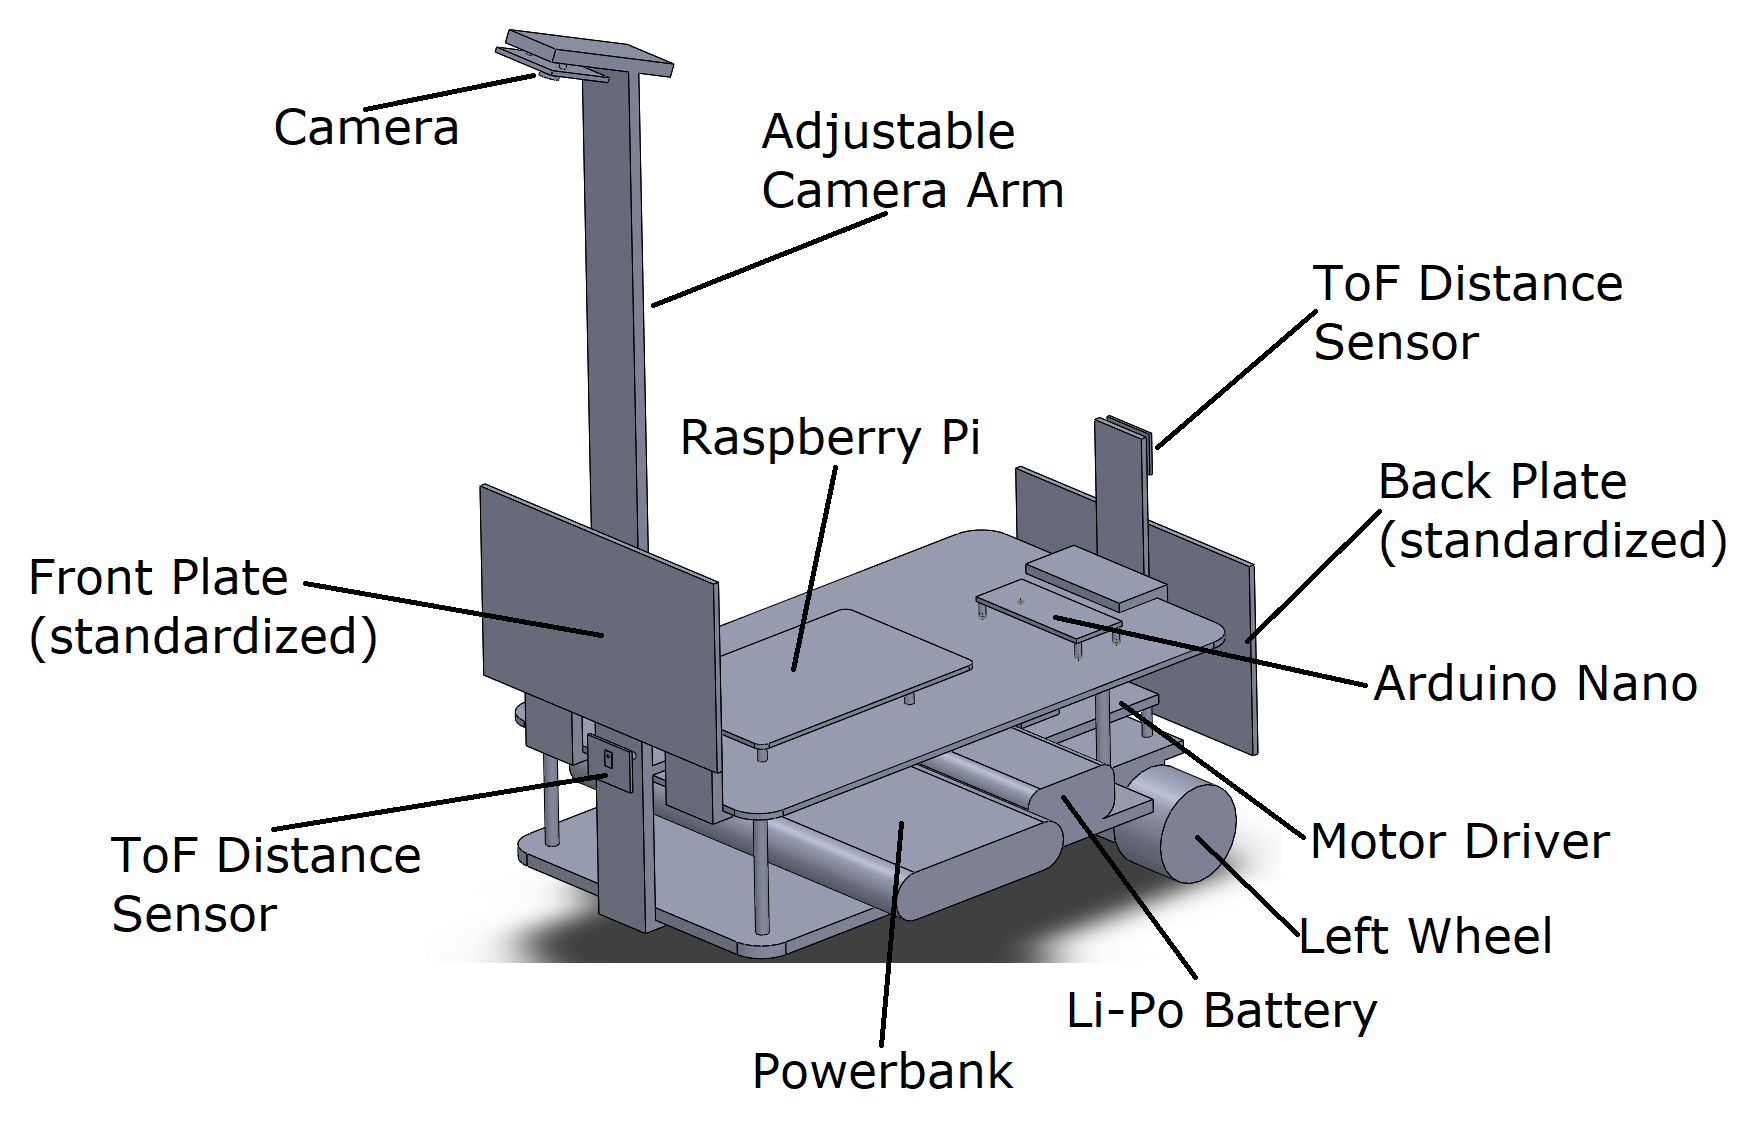
\includegraphics[width=0.8\textwidth,center]{images/chassis1}
			\caption{Isometric view of the 3D Drawing of the Vehicle \label{fig:isom} }
		\end{figure}
		\-
		\todo{choose one}
		\-
		%	\begin{figure}[H]
		%		\setlength{\unitlength}{\textwidth} 
		%		\centering
		%		\begin{subfigure}{.5\textwidth}
	  	%			\centering
	  	%			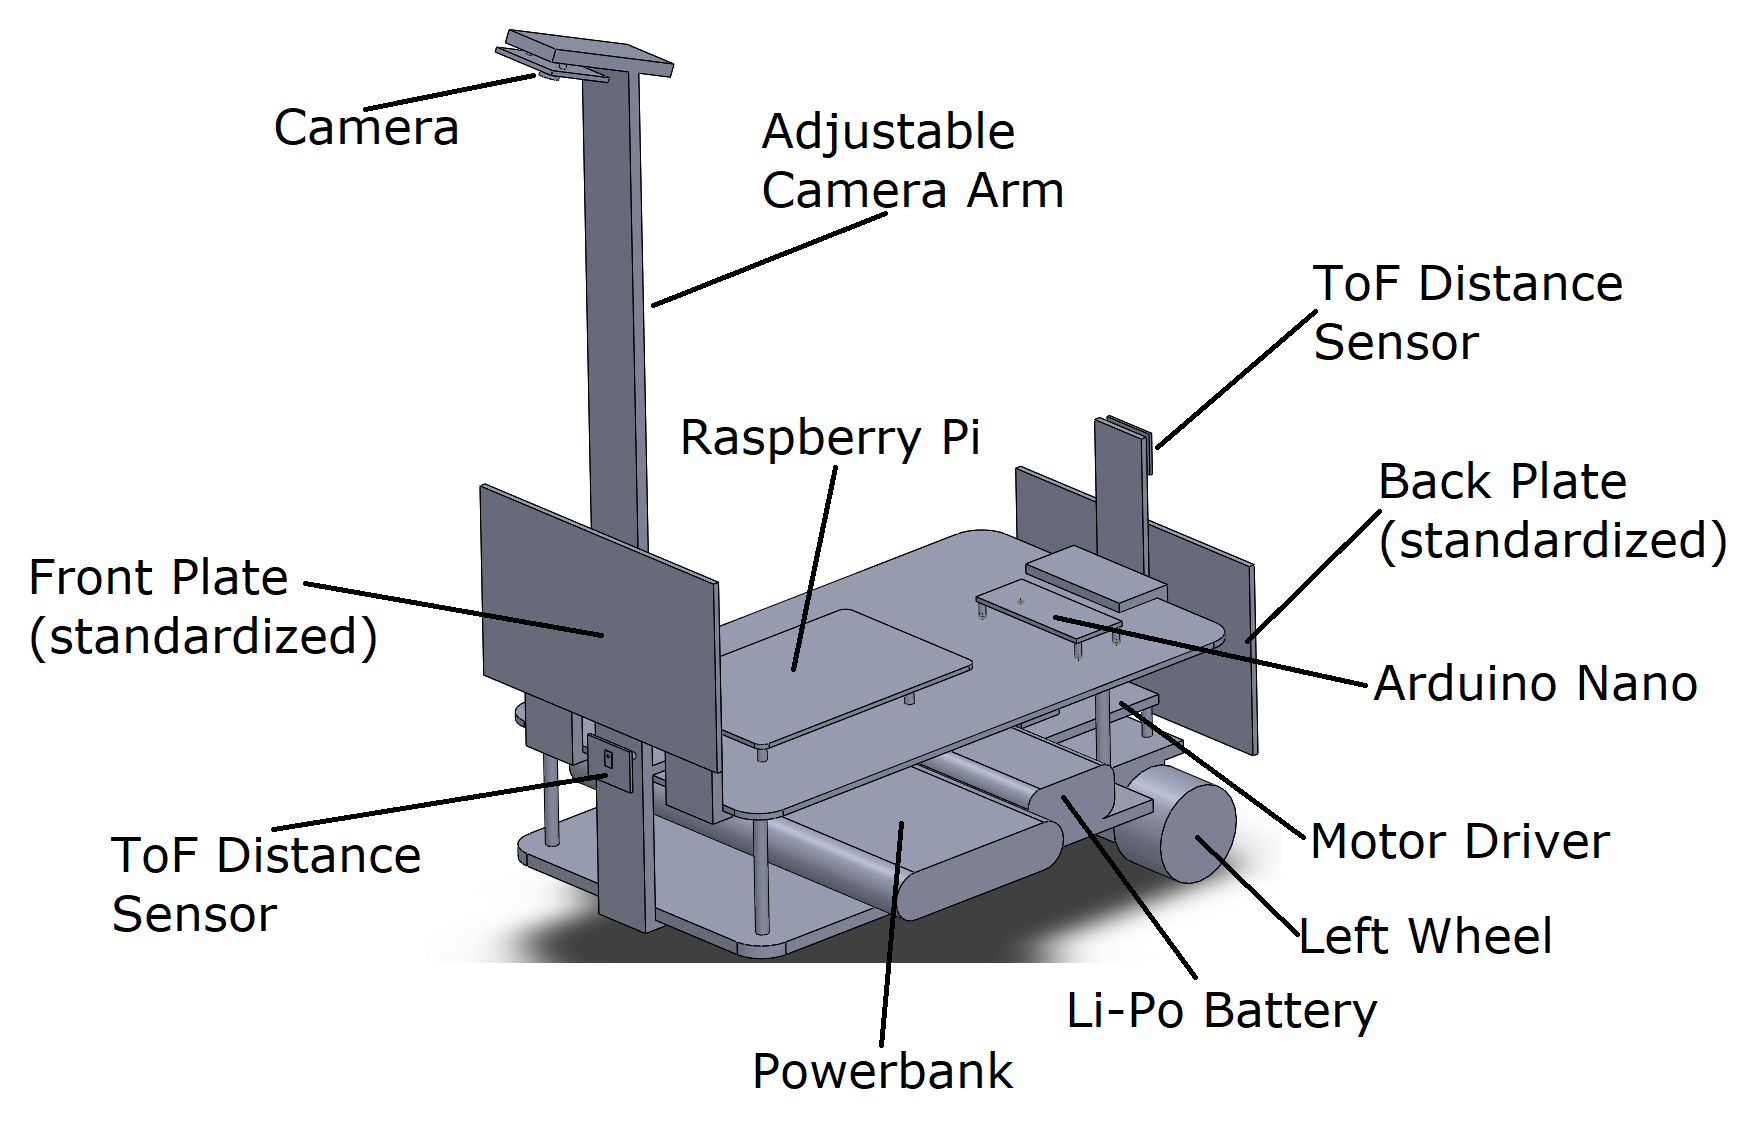
\includegraphics[width=0.48\unitlength]{images/chassis1}
	  	%			\caption{\label{fig:front-isom} Front Isometric View of the Vehicle }
		%		\end{subfigure}%
		%		\begin{subfigure}{.5\textwidth}
	  	%			\centering
		%			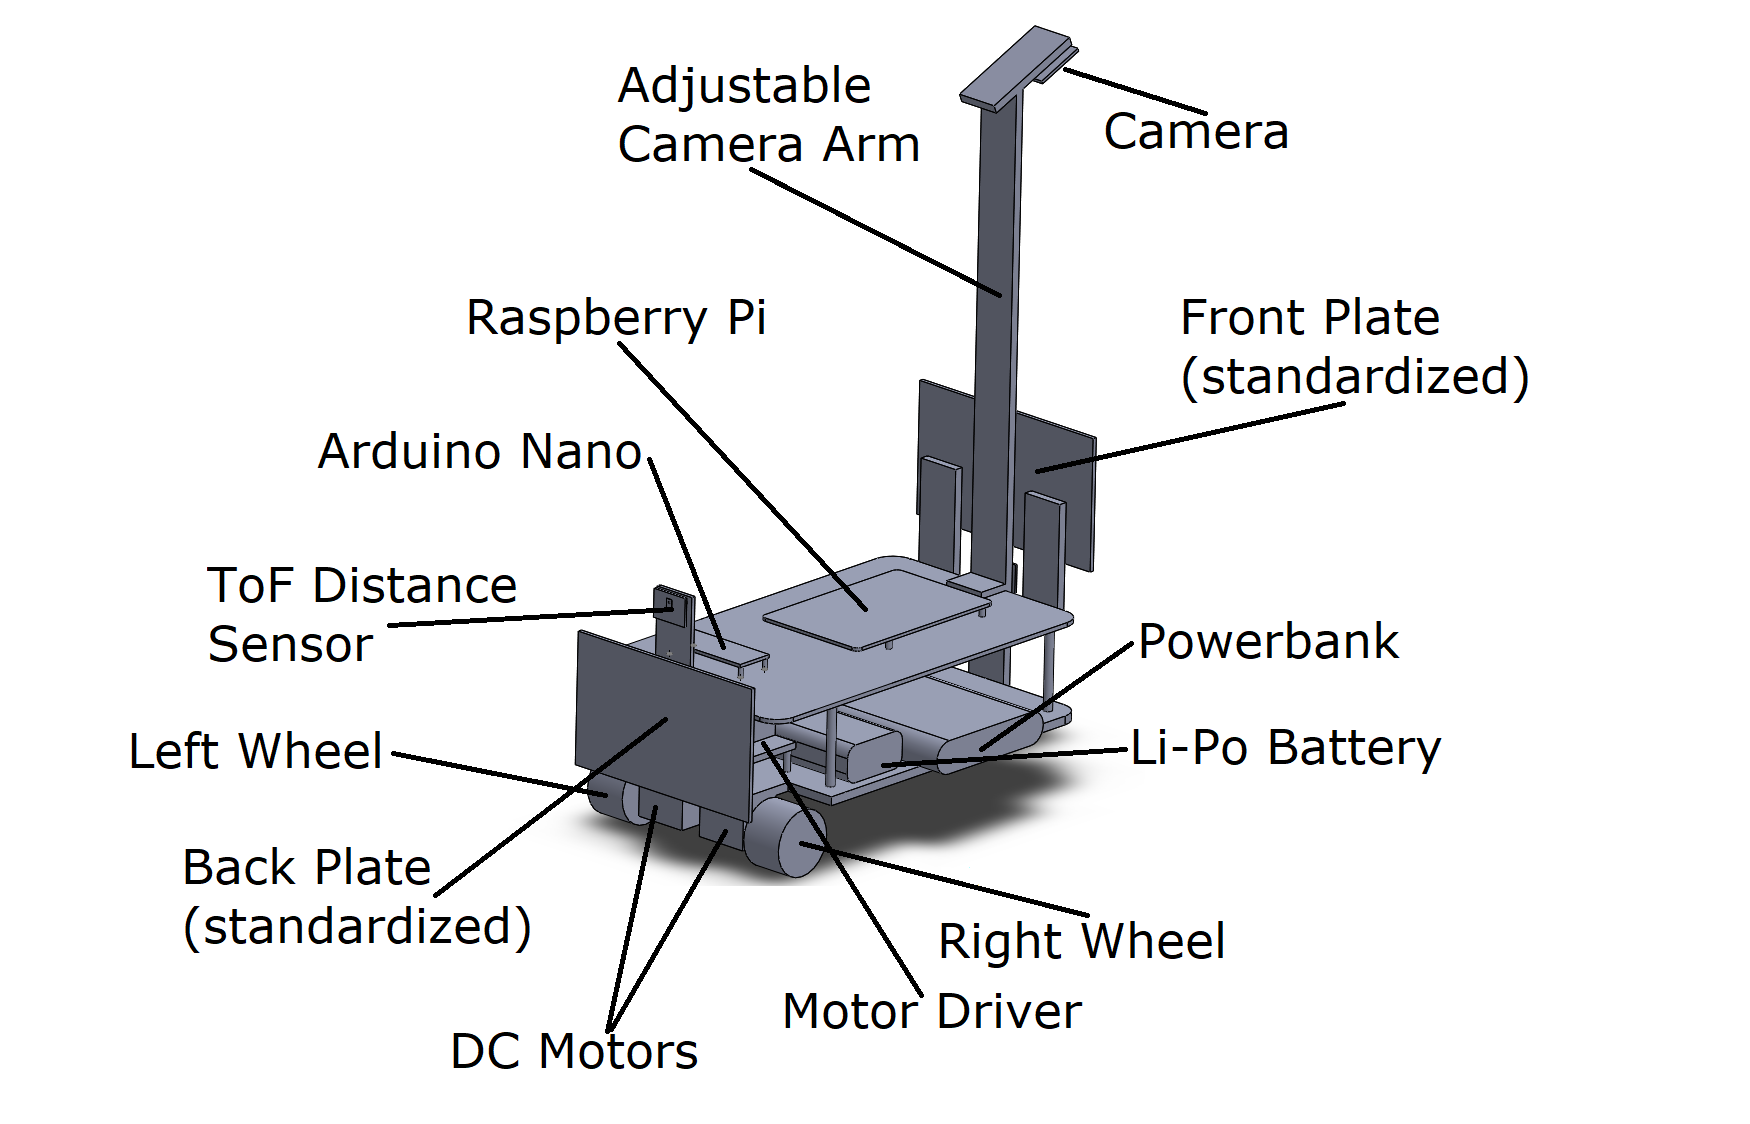
\includegraphics[width=0.48\unitlength]{images/chassis2}
	  	%			\caption{\label{fig:back-isom} Back Isometric Wiew of the Vehicle}
		%		\end{subfigure}
		%		\caption{\label{fig:isom2} Front \& Back Isometric View of the 3D Drawing of the Vehicle}
		%	\end{figure}
				
			\item {Discussions on the Solution}
			
		\end{enumerate}
			
	
	
	
	\subsubsection{Printed Circuit Board Subsystem}
	
		\begin{enumerate}
			\item {Requirements for the Solution}
			
			\begin{enumerate}
						\item The subsystem should ensure that all the electronic components are placed on PCB
						\item The subsystem should ensure that all the connections are firmly secured and robust to vibrations.
					\end{enumerate} 
					
			\item {Solution for the Subsystem}
			
			The main role of this part is decreasing connection mess and increase vibration strength of the robot against disturbances. Also, this section increases rigidity of the whole system. The requirements of this subsystem are listed below:	
	
	This subsystem aims to make all the circuit connections rigid and compact. Currently, there is wire connections between Arduino-Motor driver and Arduino-RPi. However, addition of vehicle detection sensors and other lane detection alternatives will increase the amount of components, hence, wires. In addition, to use the space occupied by the Arduino UNO board, Arduino Mini can be used. This also allows to build the circuit board as shield for Arduino Mini. After that any other sensors and connections can be made through PCB. In other words, PCB acts as a breakout board for each item integrated to the system in a more rigid and compact way.
			
			\item {Discussions on the Solution}
			
		\end{enumerate}	
	
	
	
	\subsection{Compatibility of the Subsystems}
	
	
	The block diagram showing the interaction of the subsytem block with each other can be seen from the \textit{Figure~\ref{fig:subsys-block}}. As can be seen from the figure also that, there are two main path within the project. One of them starts by processing the camera vision by the \textit{Lane Detection Subsystem} and ends with the transfer of torque from \textit{Motors Subsystem} to \textit{Wheels Subsystem} which results with a movement of the vehicle. In this path the data before the \textit{PID Controller} and \textit{Speed} subsystems are processed within the Raspberry Pi without any problem, at this point the output data are transferred to Arduino by \textit{Internal Communication Subsystem} without any problem. The rest of this path is processed by the Arduino without any problem as well.
	
	The second path starts with the detection of the opponent by the \textit{Vehicle Detection Subsystem}. The path continues within the Raspberry Pi until the \textit{vehicle stop signal} is transferred to \textit{Motors Subsystem} by \textit{Internal Communication Subsystem} without any problem.
	

	\begin{figure}[h]
		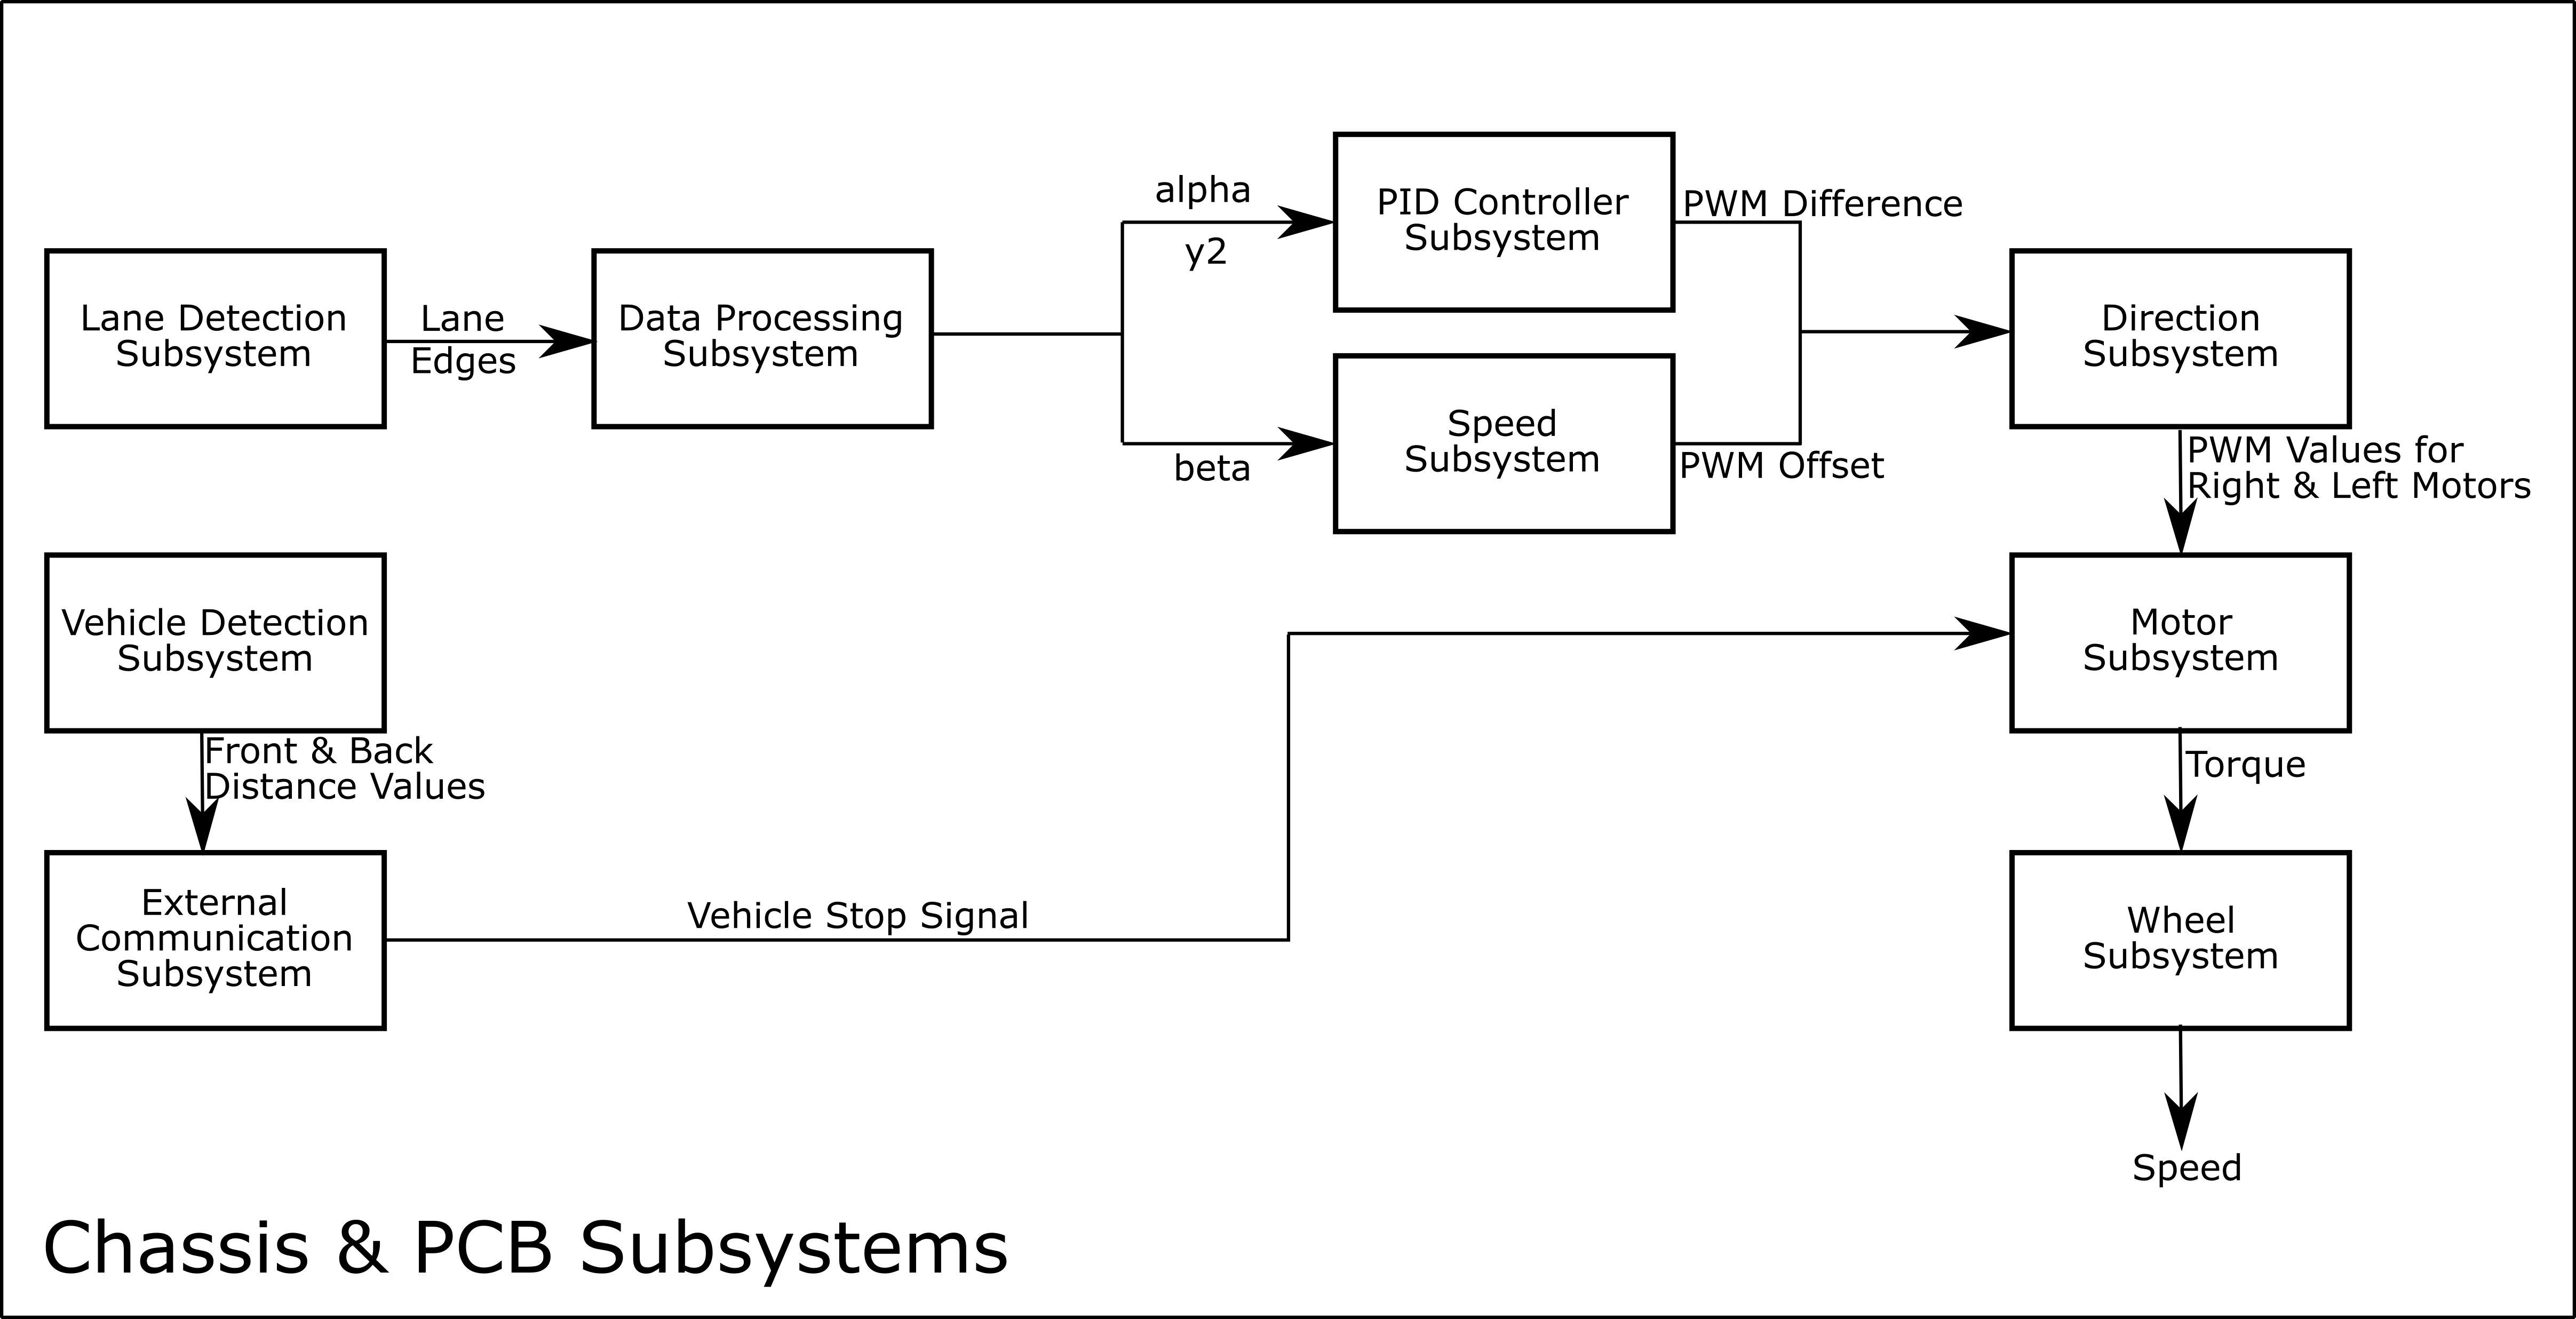
\includegraphics[width=\textwidth,center]{images/subsys_block}
		\caption{Block Diagram of the Project and the Interaction of the Subsystems}\label{fig:subsys-block}
	\end{figure}
	
%	\section{Detailed Requirements and Justifications}
	
	
		
	
	%\subsection{System \& Subsystem Requirements}

	%\begin{enumerate}
	%%%%%%%%%%%%%%%%%%%%%%%%%%%
	%\item Sensing System Requirements
	
	
	%%%%%%%%%%%%%%%%%%%%%%%%%%%	
	%\item Computation System Requirements
		
		
	%%%%%%%%%%%%%%%%%%%%%%%%%%%
	
	%\item Communication System Requirements
		
		
	%%%%%%%%%%%%%%%%%%%%%%%%%%%
	
	%\item Driving System Requirements
		
	
	%%%%%%%%%%%%%%%%%%%%%%%%%%%
	
	%\item Motion System Requirements
		
		
	%%%%%%%%%%%%%%%%%%%%%%%%%%%
	
	%\item Structure System Requirements
		
		
	%%%%%%%%%%%%%%%%%%%%%%%%%%%
	
	
	
	%\end{enumerate}

	
	%\subsection{Justifications on Design}
	
	
	
	
	
	\section{Detailed Tests for the Subsystems}\label{test_sec}
	
	\begin{enumerate}
	%%%%%%%%%%%%%%%%%%%%%%%%%%%
	\item {Lane Detection Subsystem Tests}	
	\begin{enumerate}
		\item{Light Condition Test}
				\begin{enumerate}
				\item Mirror the Raspberry Pi screen into Laptop via VNC  
				\item Execute the lane detection algorithm in Raspberry Pi 
				\item Change the location of the camera and Pi to conduct test 
				\item Observe the results in different locations   
				\item If the visible lane sides can be detected without any additional object, the result of the test can be considered as success. 
			\end{enumerate}
		\item{Visual Disturbance Test}
			\begin{enumerate}
			\item Mirror the Raspberry Pi screen into Laptop via VNC   
			\item Execute the lane detection algorithm in Raspberry Pi  
			\item Put different objects into lane  
			\item Observe the results with different disturbances 
			\item If the objects outside of lane is not detected and the objects inside the road only detected only at its border with road, the result of the test can be considered as success.  
		\end{enumerate}
	\end{enumerate}
	
	%%%%%%%%%%%%%%%%%%%%%%%%%%%
	\item {Vehicle Detection Subsystem Tests}\label{sect:vhd}
		
		\begin{enumerate}
		
		\item Front Vehicle Detection Test in Closed Environment:
			\begin{enumerate}
				\item Make the connection of the desired sensor and Arduino properly  
				\item Hold the sensor at an angle of 90 degree with respect to ground  
				\item Place the test object 5 cm in front of the desired  
				\item Observe the output of the subsystem  
				\item Repeat the step 3 \& 4 with different distances  
				\item If the output of the subsystem generates logical positive for distances smaller than 5 cm and logical zero for distances greater than five, the test result can be considered as success  
			\end{enumerate}					
		
		\item Rear Vehicle Detection Test in Closed Environment:		
			\begin{enumerate}
				\item Repeat the test steps of the \textit{Front Vehicle Detection Test in Closed Environment} with the desired sensor for the desired rear sensor.   
			\end{enumerate}
		
		\item {Angled Approach Test:}
			\begin{enumerate}
				\item Make the connection of the desired sensor and Arduino properly  
				\item Hold the sensor at an angle of 90 degree with respect to ground  
				\item Place the test object 5 cm in front of the sensor with 30 degree angle with respect to the sensor  
				\item Observe the output of the subsystem  
				\item Repeat the step 3 \& 4 with different distance and angle values  
				\item If the output of the subsystem generates logical positive for distances smaller than 5 cm for all angle values with respect to sensor and logical zero for distances greater than 5 cm, the test result can be considered as success  
			\end{enumerate}
		
		\item Vehicle Detection in Different Sunlight Conditions Test:
			\begin{enumerate}
				\item Repeat the test steps of the \textit{Front Vehicle Detection Test in Closed Environment} in CCC (Cultural and Convention) ground under direct sunlight  
				\item Repeat step 1 in CCC (Cultural and Convention) under artificial light, in other words, under no direct sunlight conditions  
				\item Repeat steps 1 \& 2 for different locations of E Building including Graduation Laboratory  
				\item If the output of the subsystem generates logical positive for distances smaller than 5 cm under all light conditions and logical zero for distances greater than 5 cm, the test result can be considered as success  
			\end{enumerate}
			
		\end{enumerate}
		
		
		%%%%%%%%%%%%%%%%%%%%%%%%%%%
		
		
		\item {Data Processing Subsystem Tests}	
		\begin{enumerate}
			\item Data Assessment Test
				\begin{enumerate}
					\item Link the output of Lane Detection subsystem to Data Processing subsystem.  
					\item Asses if the output coincide with physical reality of the path  
				\end{enumerate}
			
		\end{enumerate}
		
		
		%%%%%%%%%%%%%%%%%%%%%%%%%%%
		
		
		
		\item {PID Controller Subsystem Tests}	
	\begin{enumerate}
	
				
		\item PID Parameters Test for Given Input:		
			\begin{enumerate}
				\item Connect the Vehicle Motors to Motor Controller  
				\item Connect the Motor Driver to Arduino  
				\item Give the angle value that the subsystem should compensate   
				\item Give the power to the motors  
				\item Observe the behaviour of the vehicle  
				\item If the vehicle rotates with an angle given in step 3 without any feedback given, the result of the test can be considered as success.  
			\end{enumerate}
		
		\item Bump Test for Distance Control:
			\begin{enumerate}
				\item Set-up a lane as in \textit{Figure~\ref{fig:bump-dist}}.
				\item Make the necessary connection between motors Arduino and data processing unit  
				\item Drive the vehicle with PID parameters to be tested.
				\item Collect the distance error between the center of the lane and current position of the vehicle.
				\item Plot the time vs distance graph at Matlab using the collected distance errors.
				\item Calculate necessary performance parameters from the plot.
				
			\end{enumerate}
			
			\begin{figure}[h]
				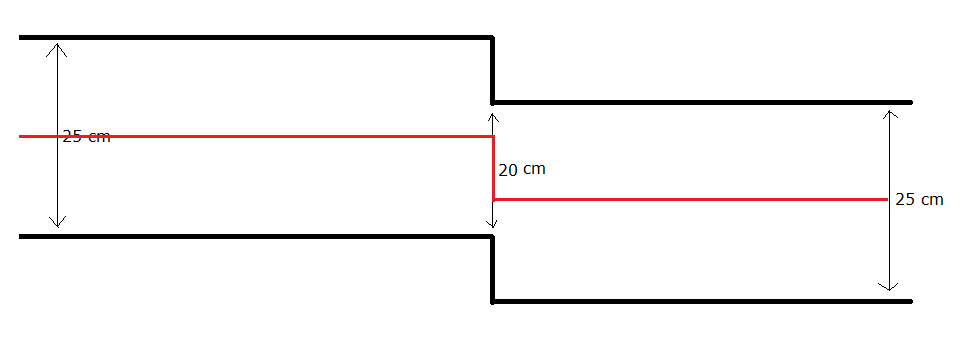
\includegraphics[width=0.75\textwidth,center]{images/bump_test_dist}
				\caption{Bump Test for Distance Control \label{fig:bump-dist} }
			\end{figure}		
			
		\item Bump Test for Angle Control:
			\begin{enumerate}
				\item Set-up a lane as in \textit{Figure~\ref{fig:bump-ang}}.
				\item Follow similar steps with \textit{Bump Test for Distance Control}, this time, however, collect the error angle information and plot accordingly.
				
			\end{enumerate}
			
			\begin{figure}[h]
				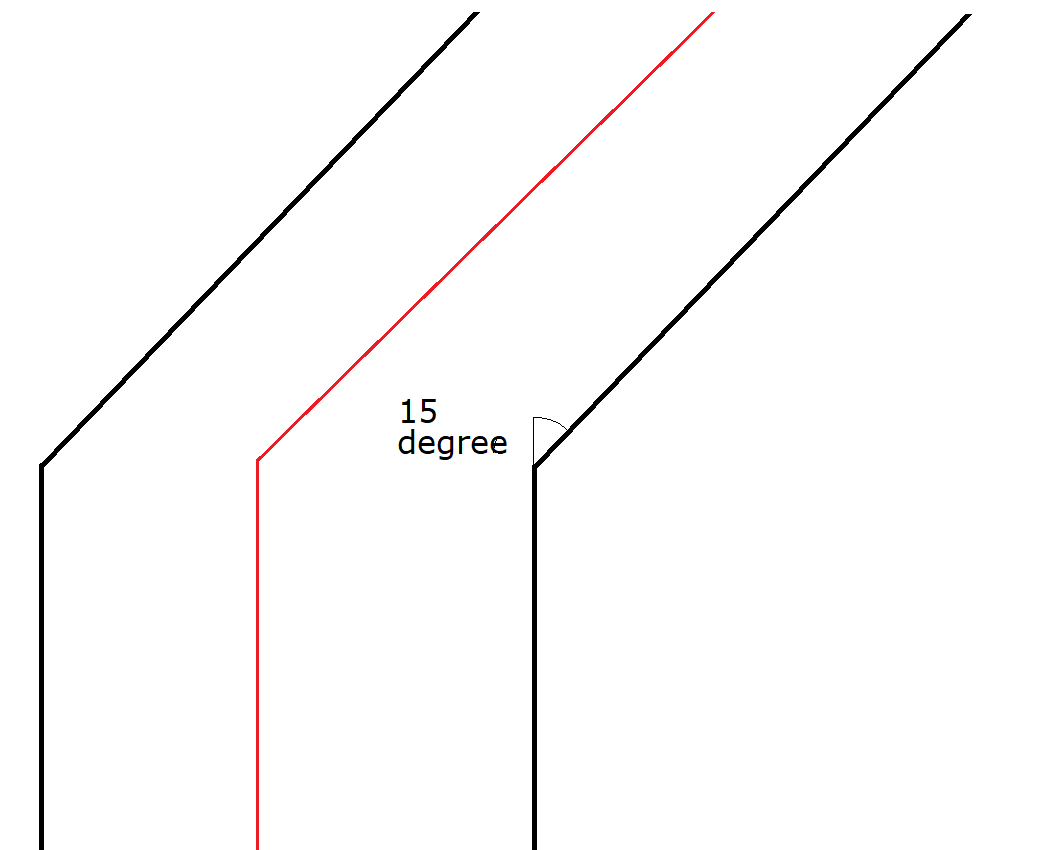
\includegraphics[width=0.45\textwidth,center]{images/bump_test_ang}
				\caption{Bump Test for Angle Control \label{fig:bump-ang} }
			\end{figure}		
		
		\item Path Tracking Test:
			\begin{enumerate}
				\item Make the necessary connection between motors Arduino and data processing unit  
				\item Place the vehicle to the desired empty path   
				\item Observe the behaviour of the vehicle  
				\item If the vehicle can follow the path smoothly, the result of the test can be considered as success.  
			\end{enumerate}
				
			
		\item Tracking a Path with Obstacles Test:	
			\begin{enumerate}
				\item Make the necessary connection between motors Arduino and data processing unit  
				\item Place the vehicle to the desired path with obstacles  
				\item Observe the behaviour of the vehicle  
				\item If the vehicle can follow the path and compensate the steady state errors due to obstacles without showing oscillatory behaviour and in a reasonable time (in less than 2 seconds), the result of the test can be considered as success.  
			\end{enumerate}
				
		
		\item Path Tracking Test with Physical Disturbances:
			\begin{enumerate}
				\item Make the necessary connection between motors Arduino and data processing unit  
				\item Place the vehicle to the desired empty path   
				\item Observe the behaviour of the vehicle  
				\item If the vehicle can follow the path and compensate the steady state errors due to physical disturbance without showing oscillatory behaviour and in a reasonable time (in less than 2 seconds), the result of the test can be considered as success.  
			\end{enumerate}
		
		\end{enumerate}
		
		%%%%%%%%%%%%%%%%%%%%%%%%%%%
		
		\item {Internal Communication Subsystem Tests}
		\begin{enumerate}
			 \item Data Retrieval Test
			\begin{enumerate}
					\item Generate data on Raspberry Pi in a rate that reflects the time consumed of Data Processing subsystem. This will yield a realistic data rate.  
				\item Send random text data to Arduino.  
				\item Do the initial integration between Arduino and Raspberry Pi.  
				\item Send data from Raspberry Pi to Arduino.  
				\item Increase data speed to the specified data rate.  
				\item Check the accuracy of the retrieved data. 
	\end{enumerate}
		\end{enumerate}
	 
	
	%%%%%%%%%%%%%%%%%%%%%%%%%%%
	
	\item {External Communication Subsystem Tests}
		
		\begin{enumerate}
		
		\item Raspberry Pi as Client Test:

			\begin{enumerate}
				\item Create a hotspot from the computer  
				\item Connect the Raspberry Pi to the hotspot  
				\item Modify the client code to be tested according to IP address of the computer
				\item Run the server code from computer  
				\item Run the client code from the Raspberry Pi  
				\item Try the possible combinations from the terminals of both sides  
				\item The test result can be considered as success if both sides respond according to the \textit{Handshake Protocol}.
			\end{enumerate}		
		
		\item Raspberry Pi as Server Test:
			
			\begin{enumerate}
				\item Create a hotspot from Raspberry Pi.  
				\item Connect the computer to the hotspot  
				\item Modify the client code to be tested according to IP address of the Raspberry Pi.  
				\item Run the server code from Raspberry Pi.  
				\item Run the client code from the computer.  
				\item Try the possible combinations from the terminals of both sides  
				\item The test result can be considered as success if both sides respond according to the \textit{Handshake Protocol}. 
			\end{enumerate}	
		
		\end{enumerate}
		
		%%%%%%%%%%%%%%%%%%%%%%%%%%%
	
	\item {Direction Subsystem Tests}
	\begin{enumerate}
	
		\item Straight Drive Test:
			
			\begin{enumerate}
				\item Make the necessary connections between motors, motor controller and the Arduino  
				\item Set the PWM values of the motors equal  
				\item Observe the behaviour of the motors  
				\item Increase the PWM value of the slower motor until a point the vehicle can go in a straight line.
				\item Record this PWM difference to use in PID controller subsystem
			\end{enumerate}
				
			
		
		\item Circular Drive Test:
			\begin{enumerate}
				\item Make the necessary connections between motors, motor controller and the Arduino  
				\item Desired curvature is decided  
				\item  According to motion of the vehicle PWMs of the motors are set  
				\item  PID parameters are set according to this test
			\end{enumerate}
		
		
	\end{enumerate}
	
	
	%%%%%%%%%%%%%%%%%%%%%%%%%%%
	
	\item {Speed Subsystem Tests}
	\begin{enumerate}
		\item Determination of the error input:
		\begin{enumerate}
			\item Make all the necessary connection
			\item Start up the vehicle
			\item Execute lane detection and controller algorithms
			\item Set the error input of the both controller algorithms the same
			\item Observe the behavior
			\item Repeat the same process with a linear function of the input
			\item Observe the success of the tracking algorithm
		\end{enumerate}
		

		\item Determination of the critical error value: 
		\begin{enumerate}
			\item Make all the necessary connection
			\item Start up the vehicle
			\item Execute lane detection and controller algorithms
			\item While the vehicle is moving, give disturbance of different types
			\item Record the maximum value of the error encountered during the disturbances.
			\item Find the maximum value
		\end{enumerate}
		
		\end{enumerate}



		%%%%%%%%%%%%%%%%%%%%%%%%%%%


		\item Wheels Subsystem Tests

		\begin{enumerate}
				\item {Handling Test:} 
				\begin{enumerate}
					\item  Place the vehicle on the path
					\item Apply a horizontal force
					\item Observe the behaibour 
					\item If the vehicle is slipping, the test can be considered to be failure. If not, the the test result can be considered as success. In other word, friction between road and wheel should greater than road and ground. 

				\end{enumerate}
		\end{enumerate}

		\item Motors Subsystem Tests

		\begin{enumerate}
				\item {Torque Test:} 
				\begin{enumerate}
					\item Fix the motor at horizontal position with respect to ground  
					\item Attach an object of one kilogram  
@@ -1070,9 +1091,10 @@
					\item Contact the seller for more information 
				\end{enumerate}
		\end{enumerate}
		
		
		
		
			
		
		
		%%%%%%%%%%%%%%%%%%%%%%%%%%%
	
	\item {Chassis Subsystem Tests}
	\begin{enumerate}
		\item Inertia test: 
		\begin{enumerate}
		\item Prepare a straight path
		\item Power up the vehicle 
		\item Execute the edge detection and control algorithm
		\item Give different type of disturbances 
		\item Observe the deviation from straight line
		\item Repeat the process with different component configurations
		\end{enumerate} 
	\end{enumerate}
	
	
	
	
	%%%%%%%%%%%%%%%%%%%%%%%%%%%

	
	\item {Printed Circuit Board Subsystem Tests}
	
	\begin{enumerate}
		\item Short test: Aims to check all the wanted connections are present. The test procedure is as follows:
		\begin{enumerate} 
			\item Open multimeter for short circuit test  
			\item Find the ends of each routing 
			\item Check the continuity using multimeter probes
			\item Check if there is any unwanted short circuit
			\item If exist, eliminate
		\end{enumerate}
	\end{enumerate}
	
	
	
	\end{enumerate}
		
	
	
	\section{Testing Stage}
	
	\subsection{Test Results, Encountered Problems and Possible Solutions for Subsystems}	
	
	\subsubsection*{Results of Lane Detection Subsystem Tests}
		
	The lane detection tests were conducted for the detection algorithm of the camera. A sample test result is shown in \textit{Figure~\ref{fig:laneD_test}}. The tests reveal that the subsystem satisfies its requirements by detecting edges. Note that, not all lines are detected, only the lines that are in the ROI are detected as discussed in \textit{Section~\ref{sec:LaneDetectionSubsystem}}.
	
				\begin{figure}[h]
		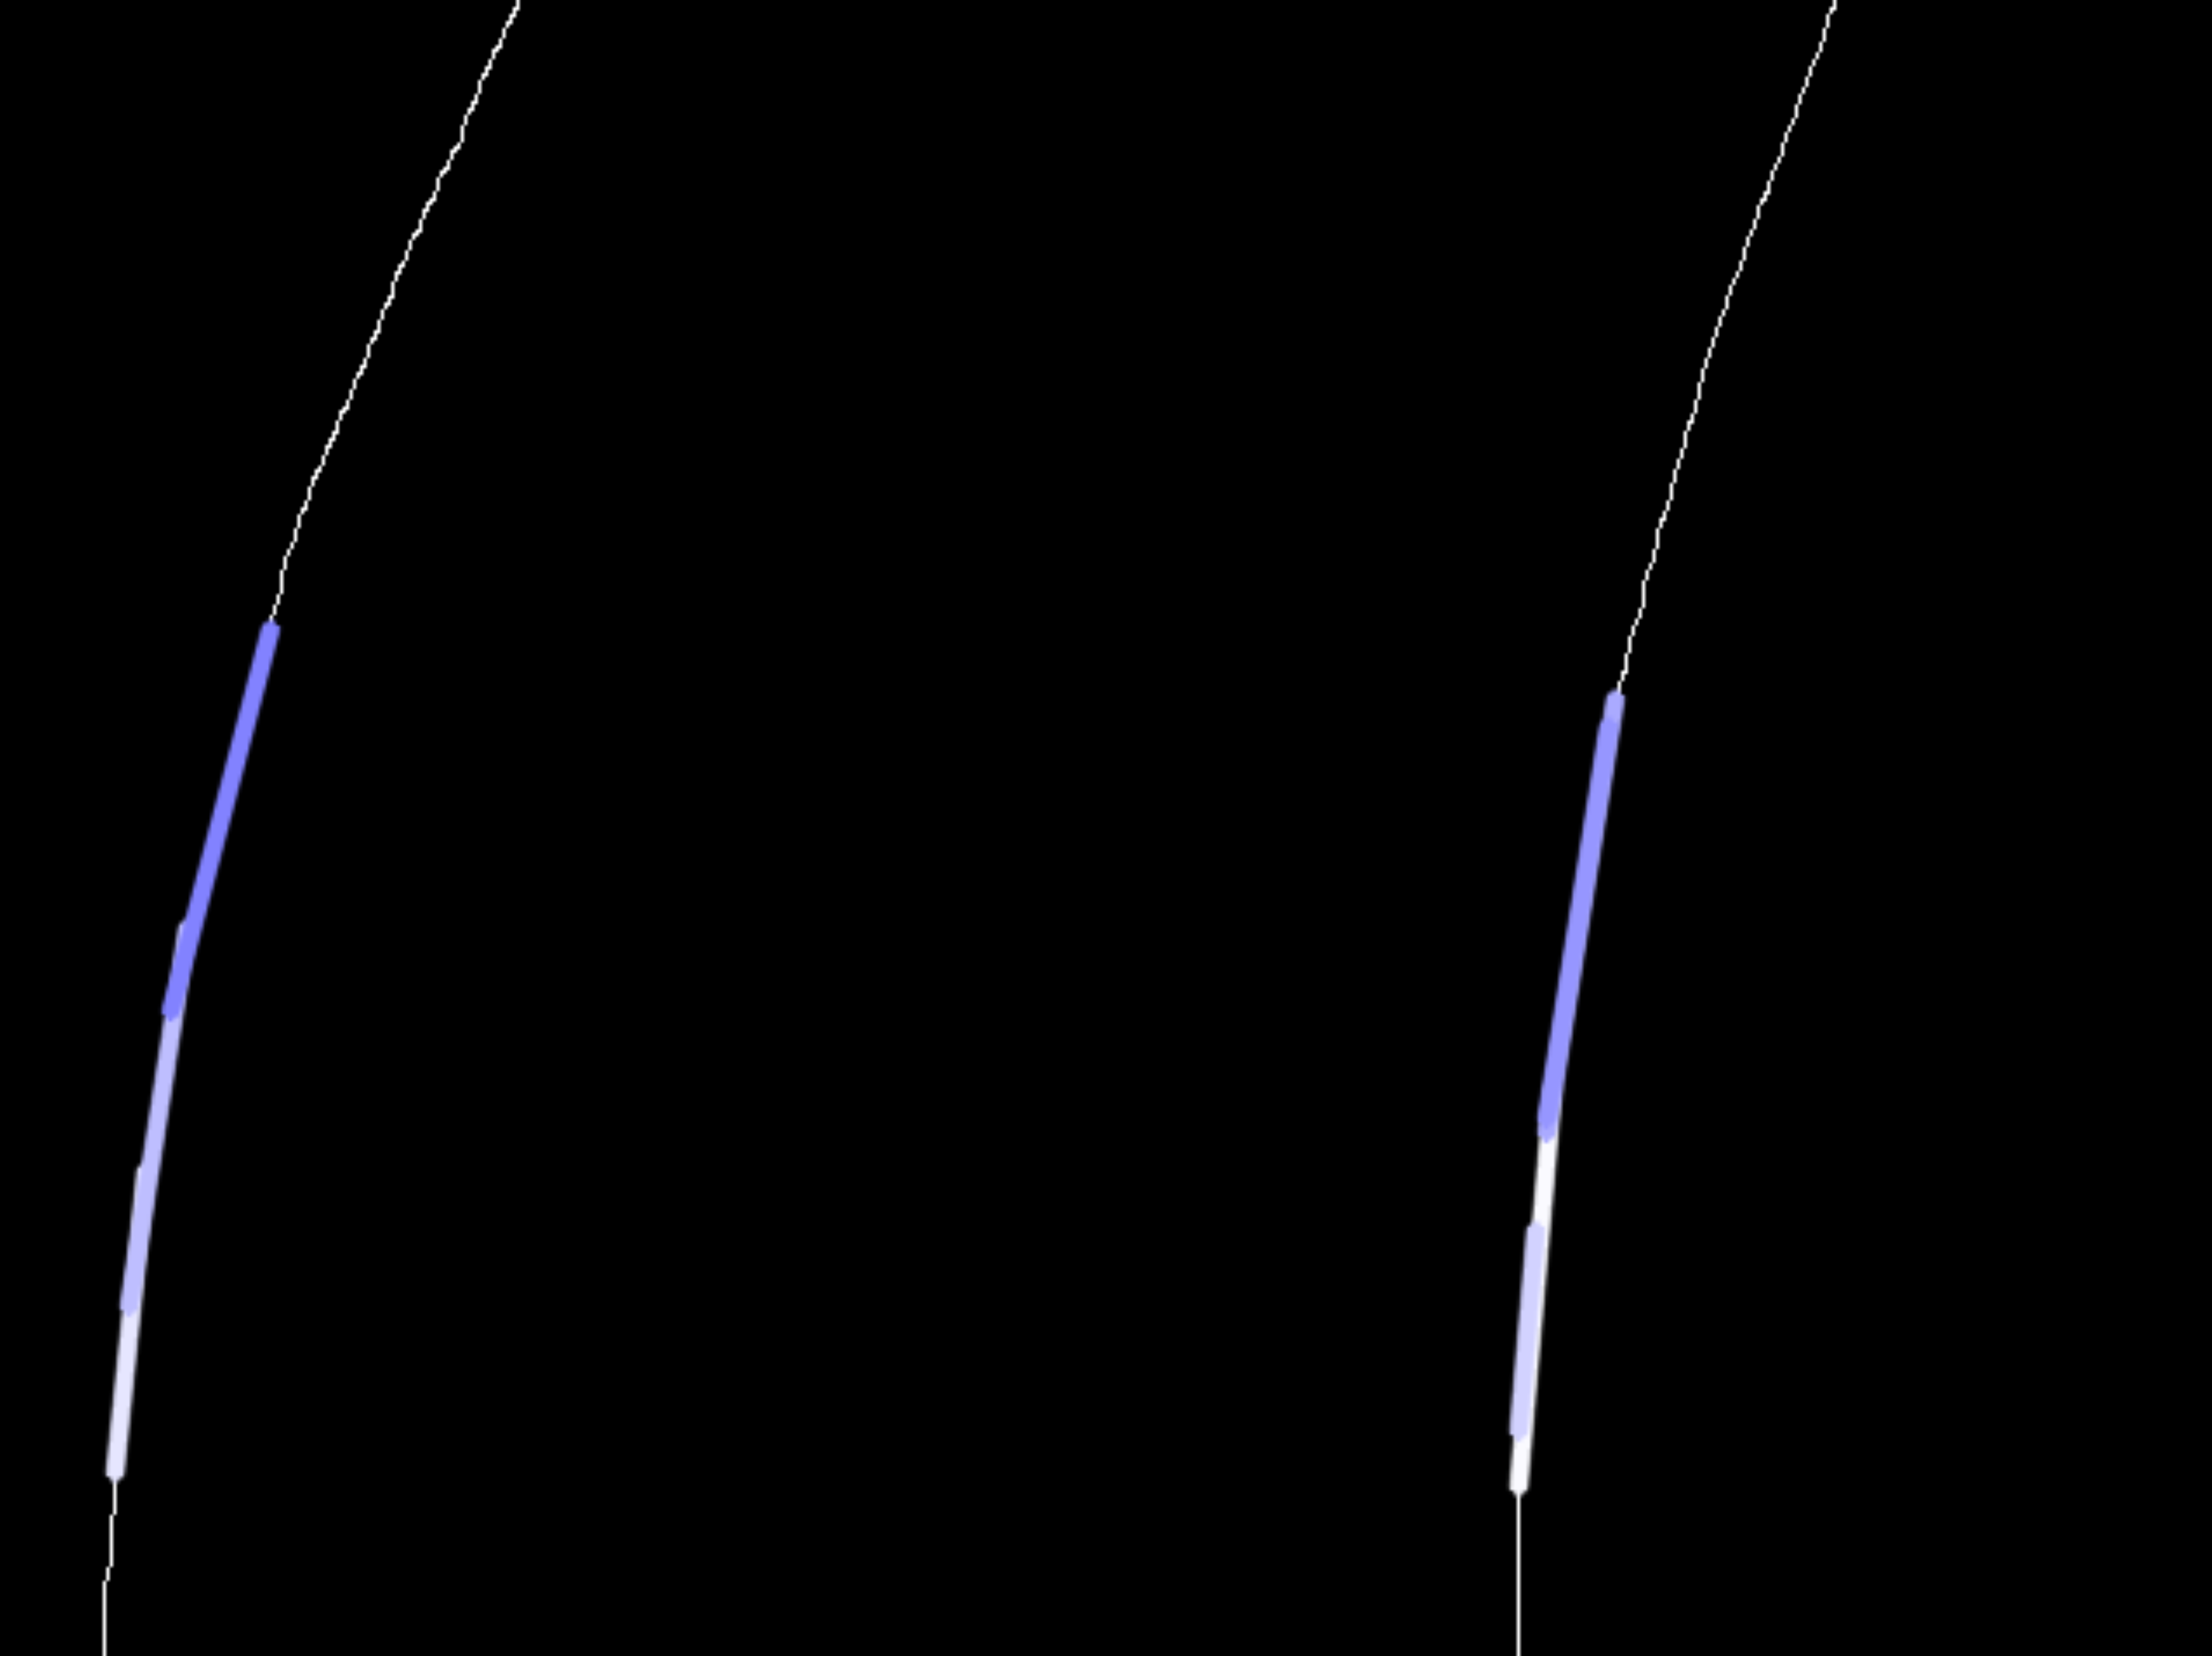
\includegraphics[width=0.75\textwidth,center]{images/laneD_test}
		\caption{Lane Detection Test Result \label{fig:laneD_test} }
	\end{figure}
		
	
	
	\subsubsection*{Results of Vehicle Detection Subsystem Tests}
	
		All the test procedures mentioned at the \textbf{Section~\ref{sect:vhd}} were applied to the ultrasonic sensor (HC-SR04) and two infrared sensors (TCRT5000 \& QRD1114). The ultrasonic sensor were showed very inaccurate result especially in \textit{Angled Approach Test}. The test results can be examined at \textit{Table`\ref{tab:aat}}. Considering the fact that the path itself is elliptical and there would always be an angle between vehicle even though it may be very small for some cases, it was decided that ultrasonic sensors are not a good choice for this subsystem. However, it is always possible that these sensors can be supportive sensors for the subsystem.
		
		\begin{table}[H]
		  \centering
		  	\caption{The Results for the Angled Approach Test for HC-SR04}
		    \begin{tabular}{c|c|c}
    		   $$Actual Distance$$ & $$The Angle$$ & $$Measured Distance$$ \\ \hline
			   3  cm & 90 & 3.15 cm  \\ \hline
    		   5  cm & 90 & 5 cm  \\ \hline
    		   20 cm & 90 & 20.01 cm  \\ \hline
    		   40 cm & 90 & 40.25 cm \\ \hline
       		   5  cm & 45 & 6.78 cm \\ \hline
    		   20 cm & 45 & 28.8 cm  \\ \hline
       		   30 cm & 45 & 42.4 cm  
  			\end{tabular}
  			\label{tab:aat}
		\end{table}
		
		 Unlike ultrasonic sensors, infrared sensors showed very accurate result inside the closed environments like laboratory under artificial lights. However, the results under direct sunlight especially in CCC were not as good as expected.  Thus, it was decided that the main solution should be an enhanced version of infra-red sensors namely the ones utilizing the "time-of-flight" concept. Moreover, laser sensors might be good alternative for these subsystems.
	
	
		
	
		
		
		
	\subsubsection*{Results of Data Processing Subsystem Tests}\label{sec:DataProcessingSubsystemTests}
	The tests in this section assesses the ability and performance of this subsystem by regarding its requirements. The number of tests realized is quite  bit. The first set of tests cover the robustness of the subsystem by placing an obstacle of the subsystem. This test and its results are presented in \textit{Figure~\ref{fig:dataP_down},\ref{fig:dataP_up} and \ref{fig:dataP_par}}. It can be seen that the algorithm ignores the obstacles in 7 cases out of 9 tests. In two cases, the algorithm fails to ignore the obstacles and determines the steering angle as if obstacle constitutes the lane line. Besides the results, on the presence of obstacles, in some particular obstacle placements, the output of the subsystem is observed to be unstable.
	
	The second set of tests cover the robustness of the subsystem as well, but under changing lighting conditions and on different surface materials. The results of this test is presented in \textit{Figure~\ref{fig:dataP_inside} and \ref{fig:dataP_outside}}. The presented results are promising, the steering angles are true. A problem is that these results are a bit unstable when the luminosity difference between the shadows and flighty parts increase. The shadows are sometimes detected as lines and cause untrue lane line evaluations.	
	
	\begin{figure}[H]
	\setlength{\unitlength}{\textwidth} 
	\centering
	\begin{subfigure}{.31\textwidth}
		\centering
		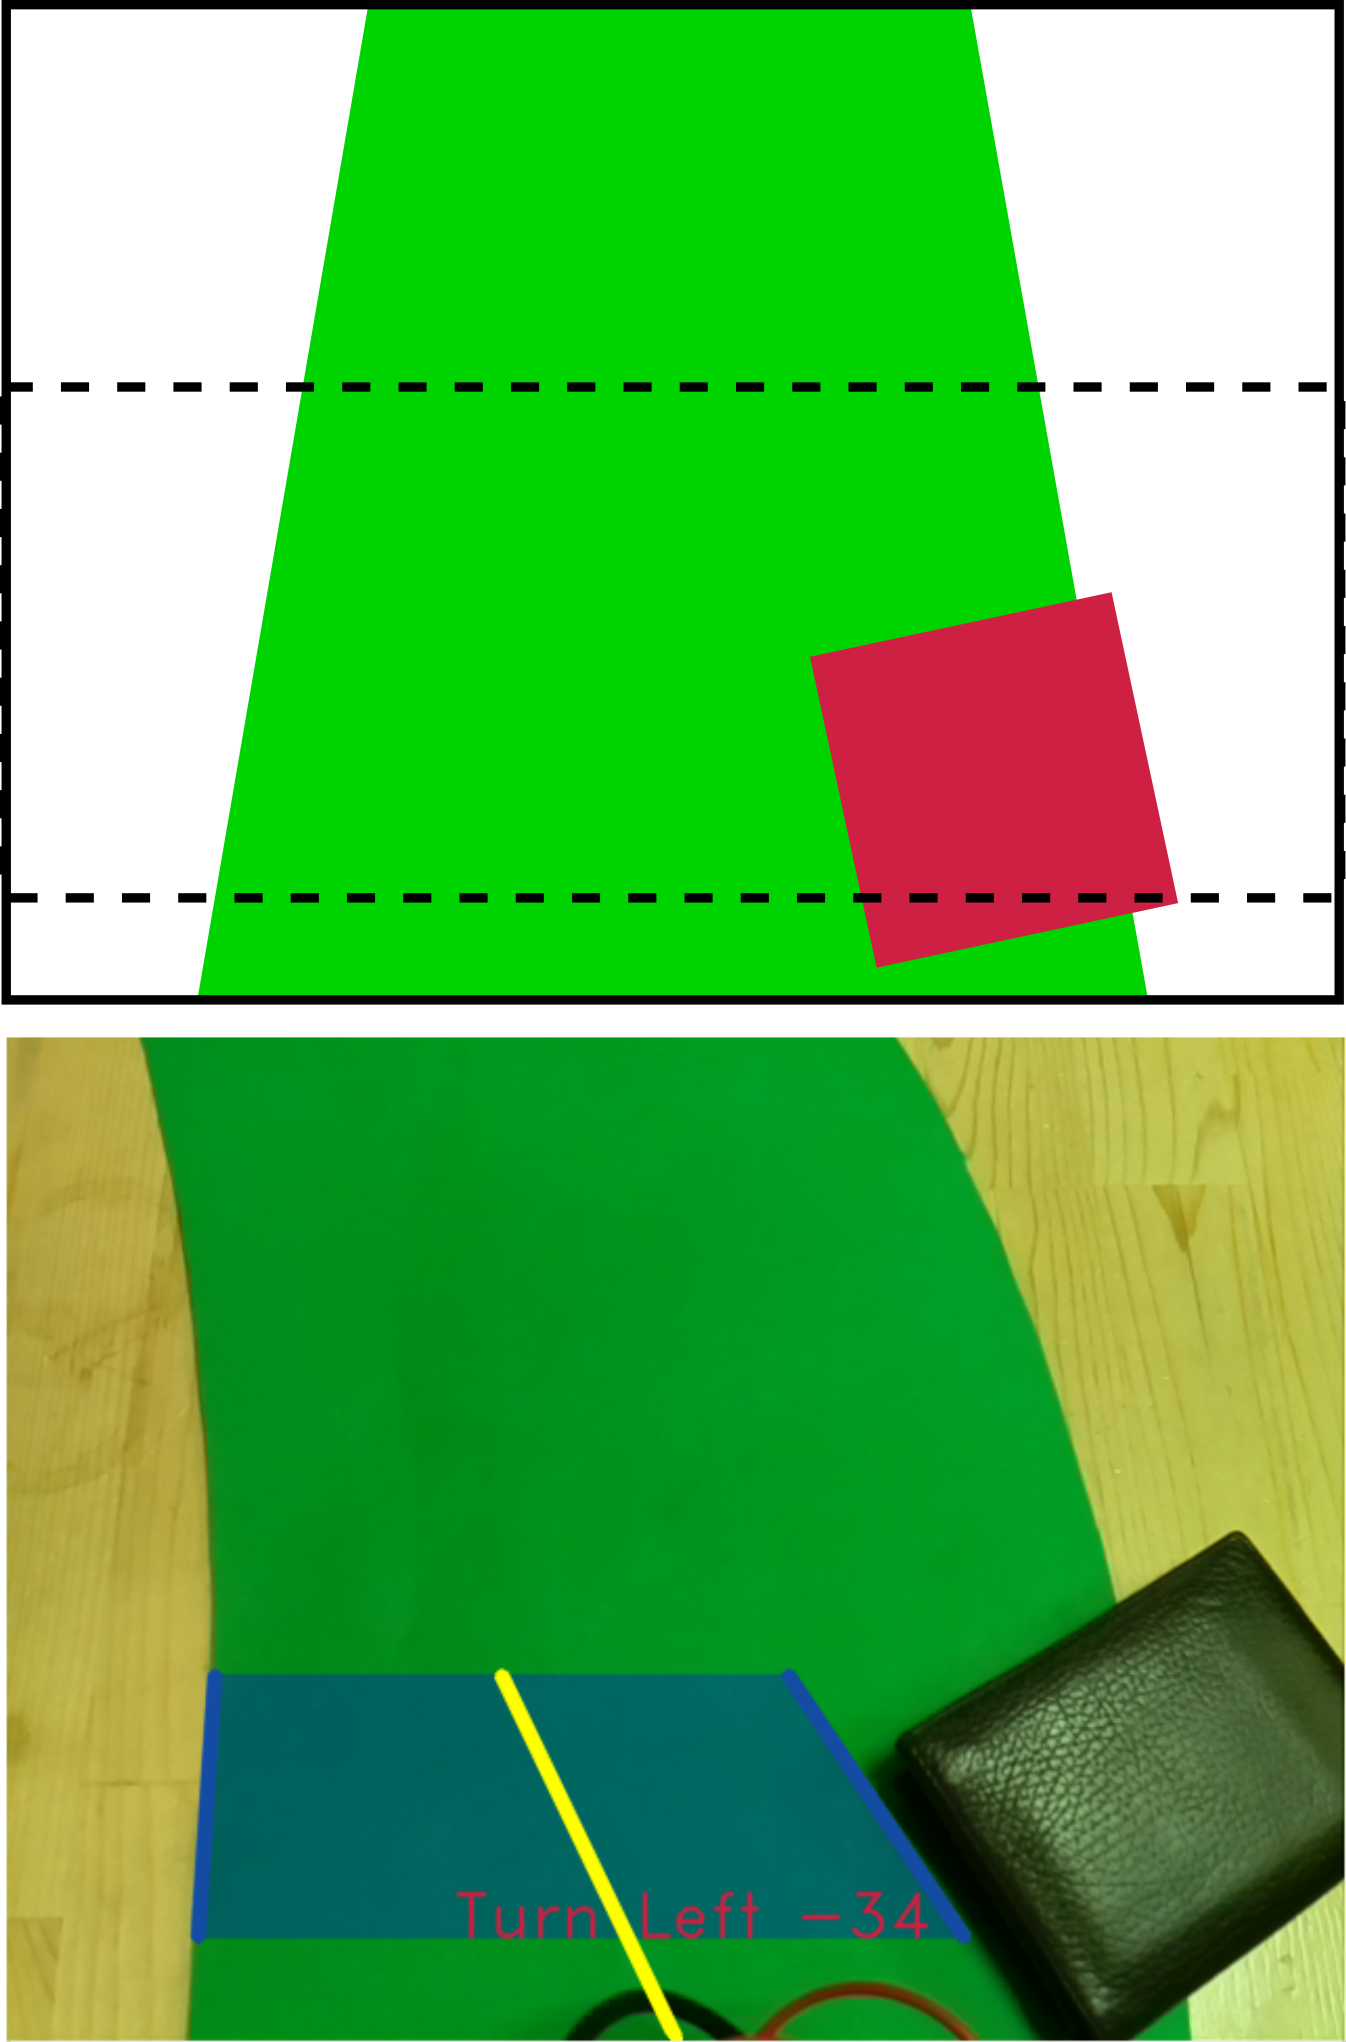
\includegraphics[width=0.30\unitlength]{images/path_images/down_1}
		\caption{\label{fig:dataP_down_1} Obstacle is at the Beginning of the Path}
	\end{subfigure}%
	\begin{subfigure}{.31\textwidth}
		\centering
		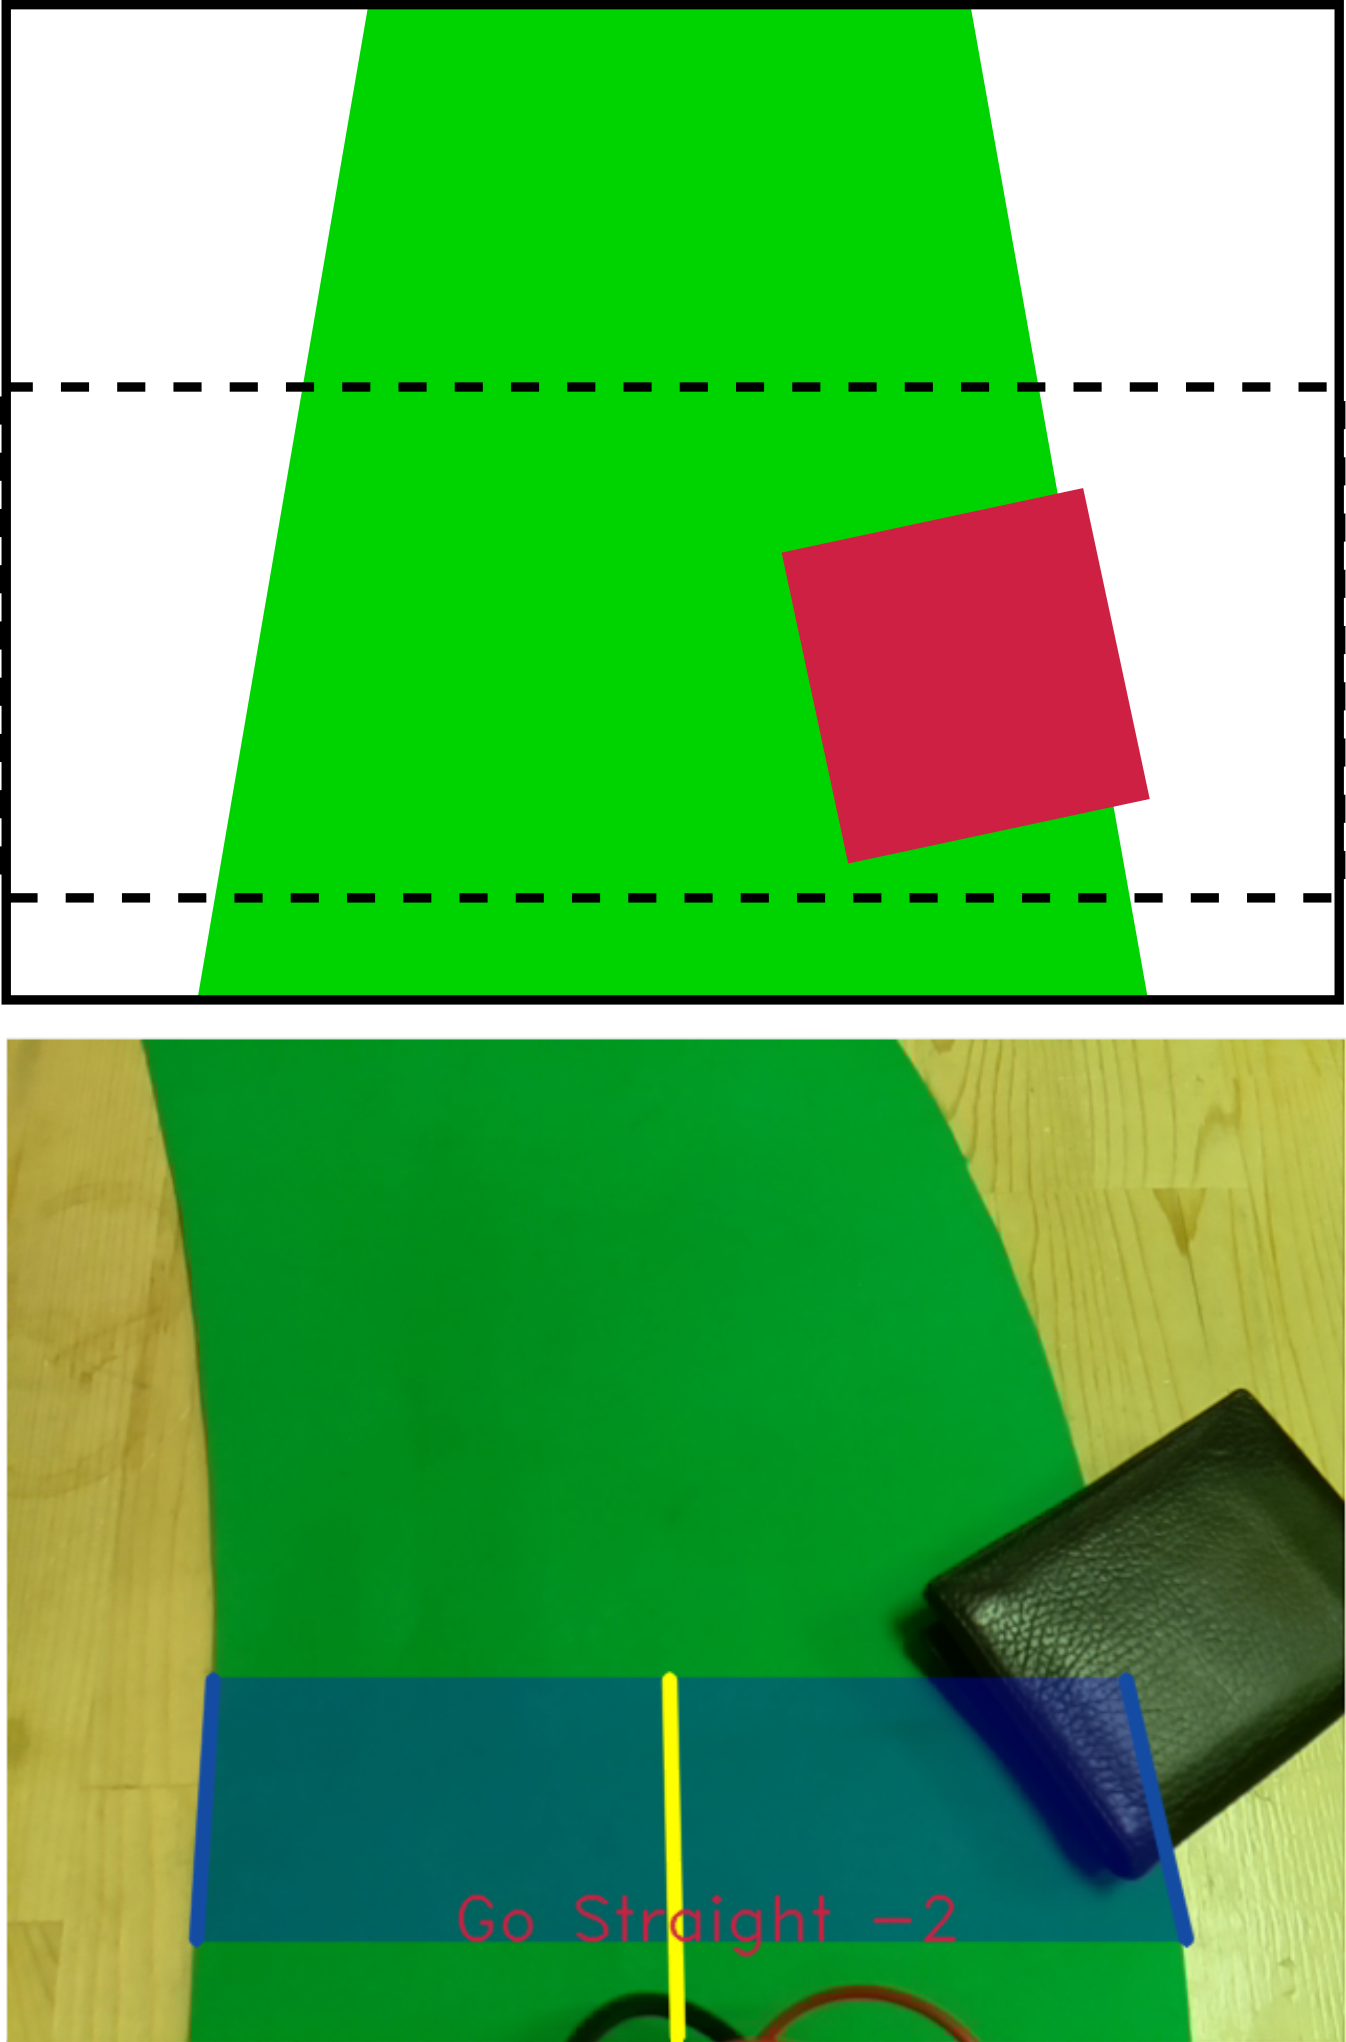
\includegraphics[width=0.30\unitlength]{images/path_images/down_2}
		\caption{\label{fig:dataP_down_2} Obstacle is at the Middle of the Path}
	\end{subfigure}
		\begin{subfigure}{.31\textwidth}
		\centering
		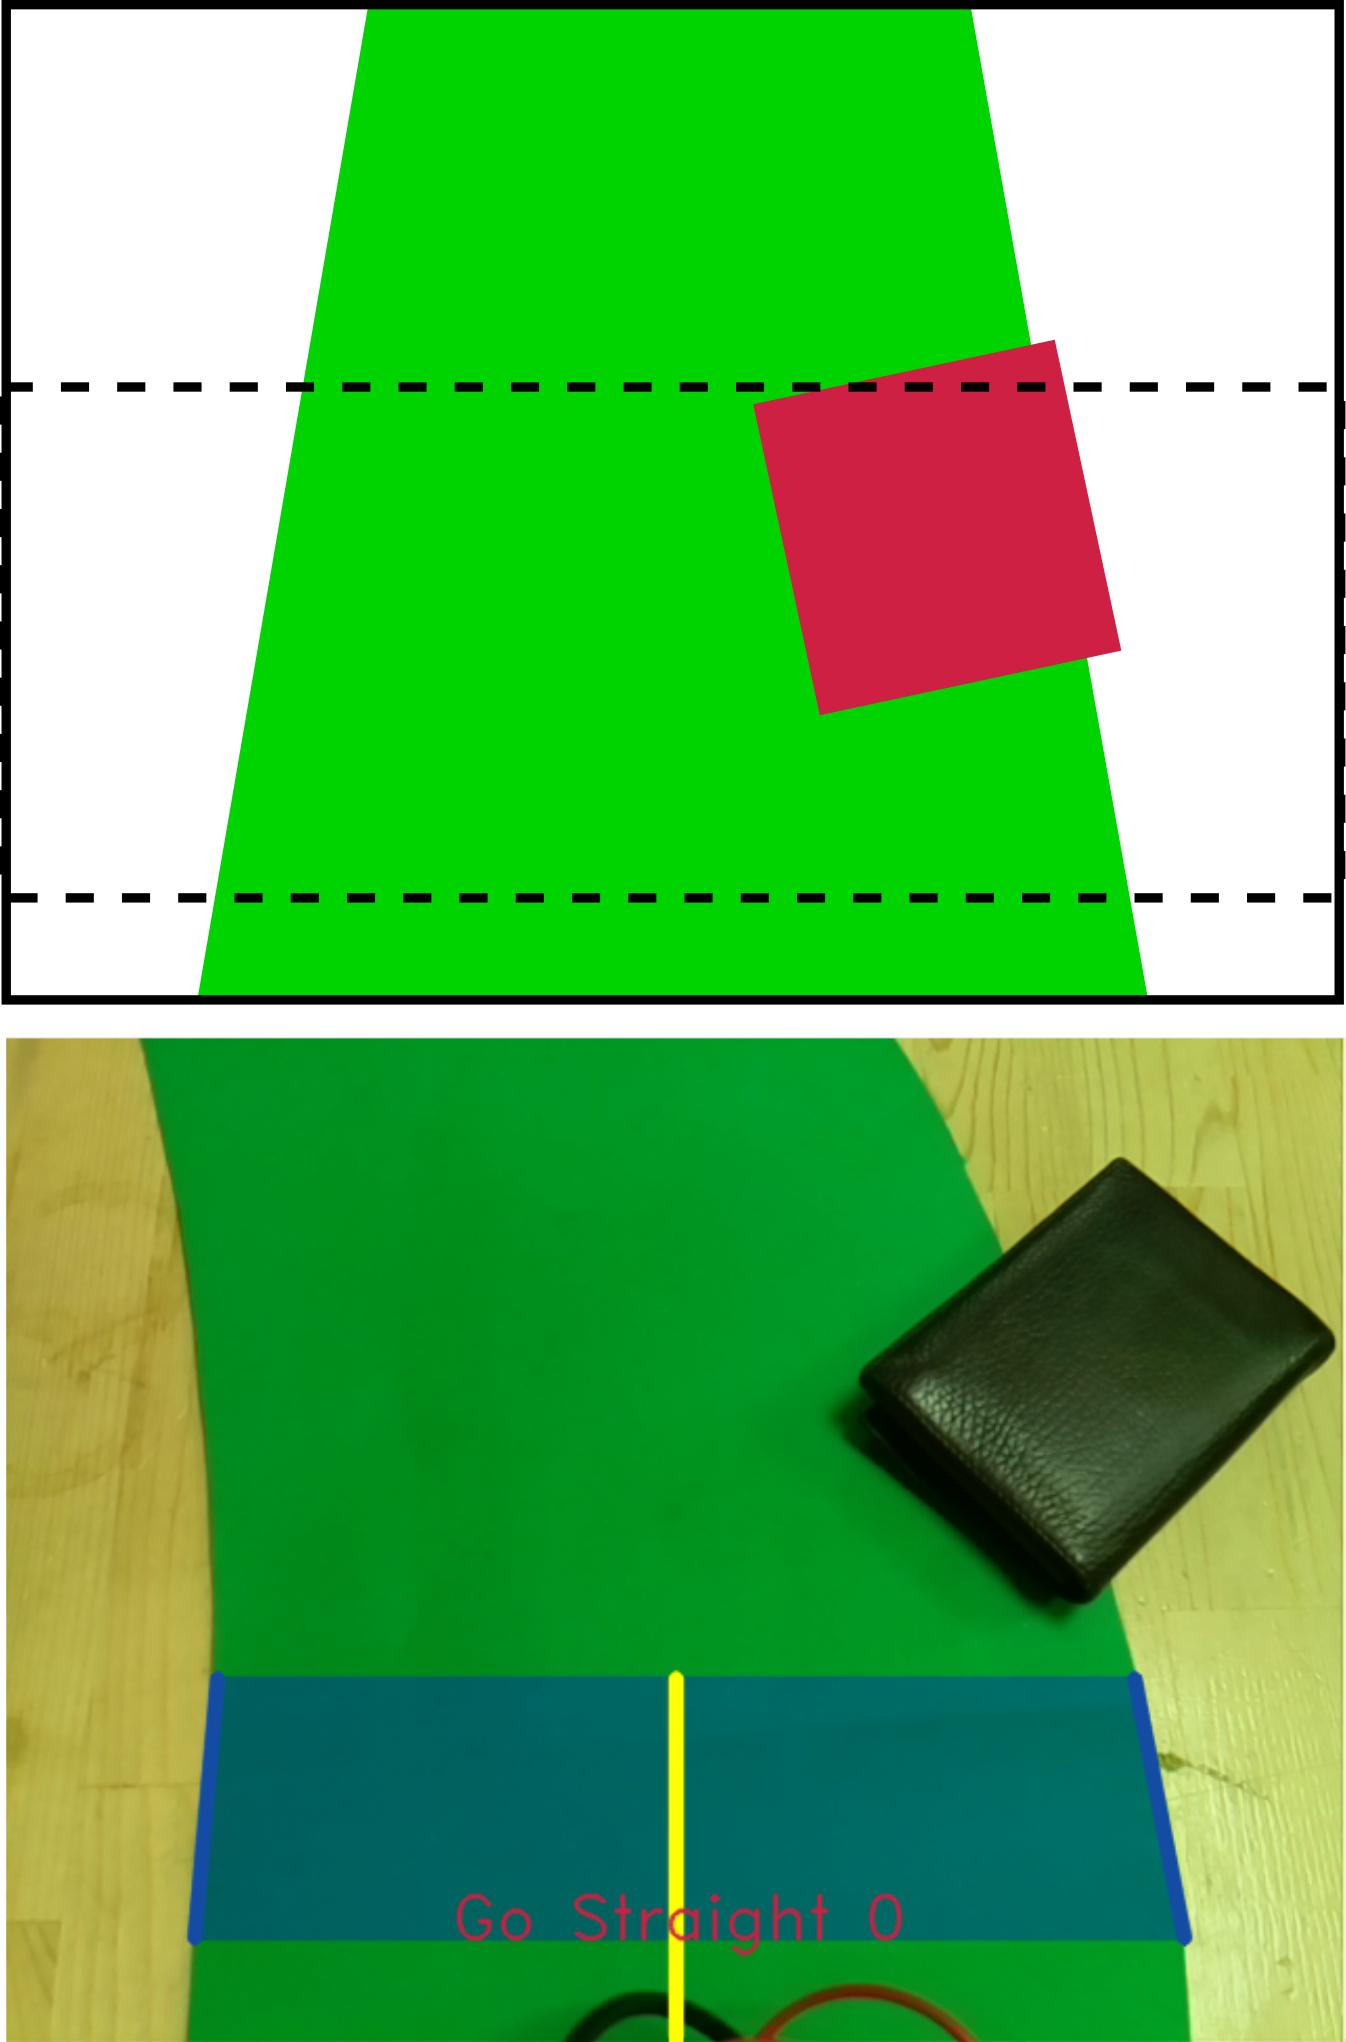
\includegraphics[width=0.30\unitlength]{images/path_images/down_3}
		\caption{\label{fig:dataP_down_3} Obstacle is at the End of the Path.}
	\end{subfigure}
	\caption{\label{fig:dataP_down} A Test Scenario: Downward Inclined Obstacle on the Path. \\ Upper Half: Proposed Tests, Lower Half: Results}
\end{figure}
	
	\begin{figure}[H]
	\setlength{\unitlength}{\textwidth} 
	\centering
	\begin{subfigure}{.31\textwidth}
		\centering
		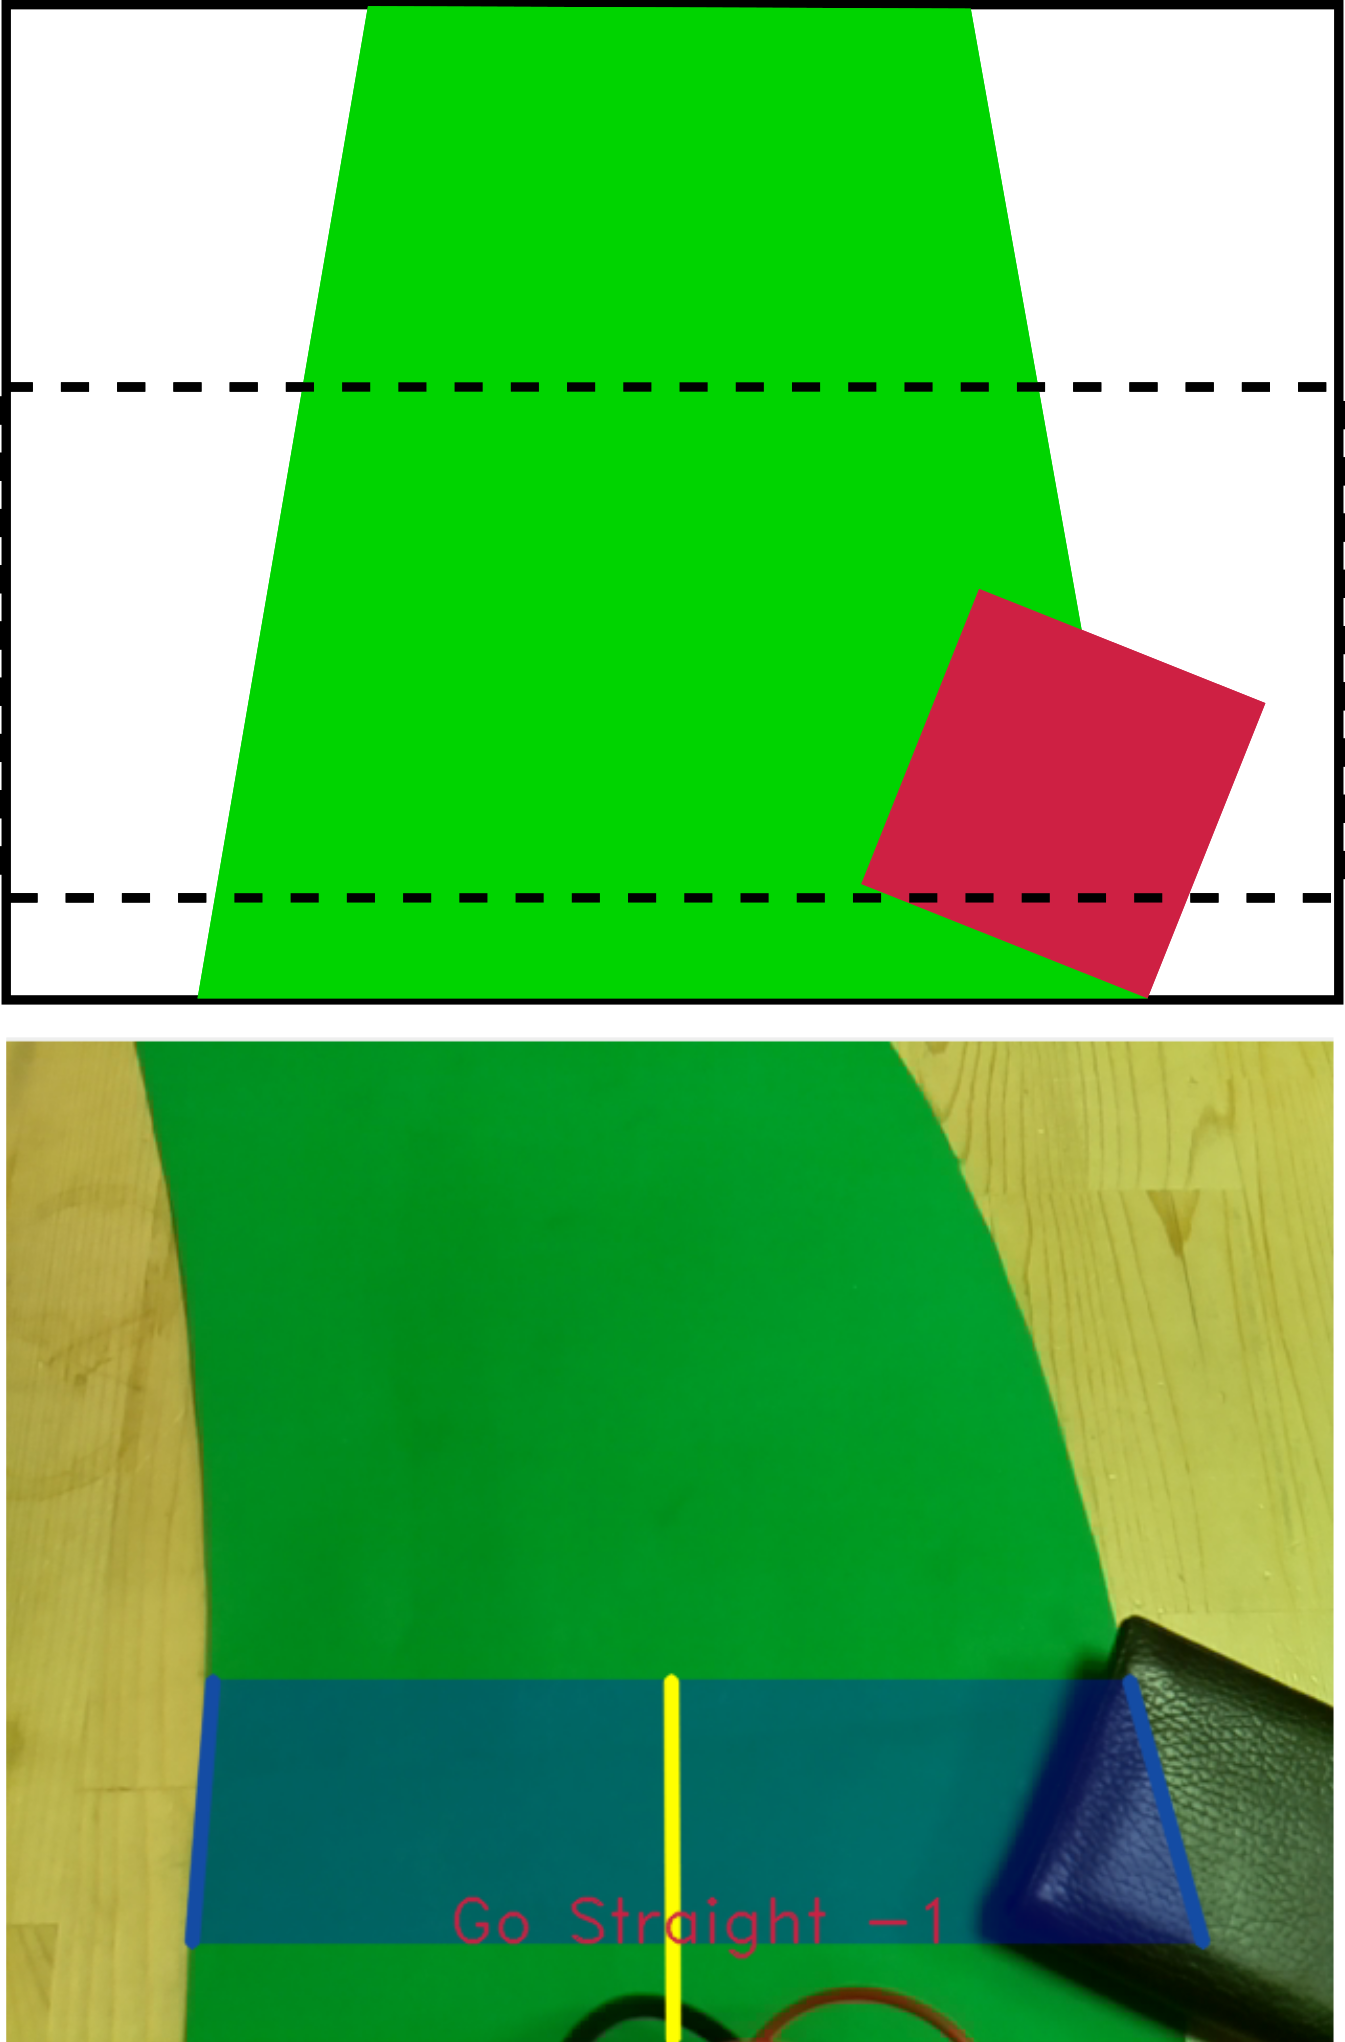
\includegraphics[width=0.30\unitlength]{images/path_images/up_1}
		\caption{\label{fig:dataP_up_1} Obstacle is at the Beginning of the Path}
	\end{subfigure}%
	\begin{subfigure}{.31\textwidth}
		\centering
		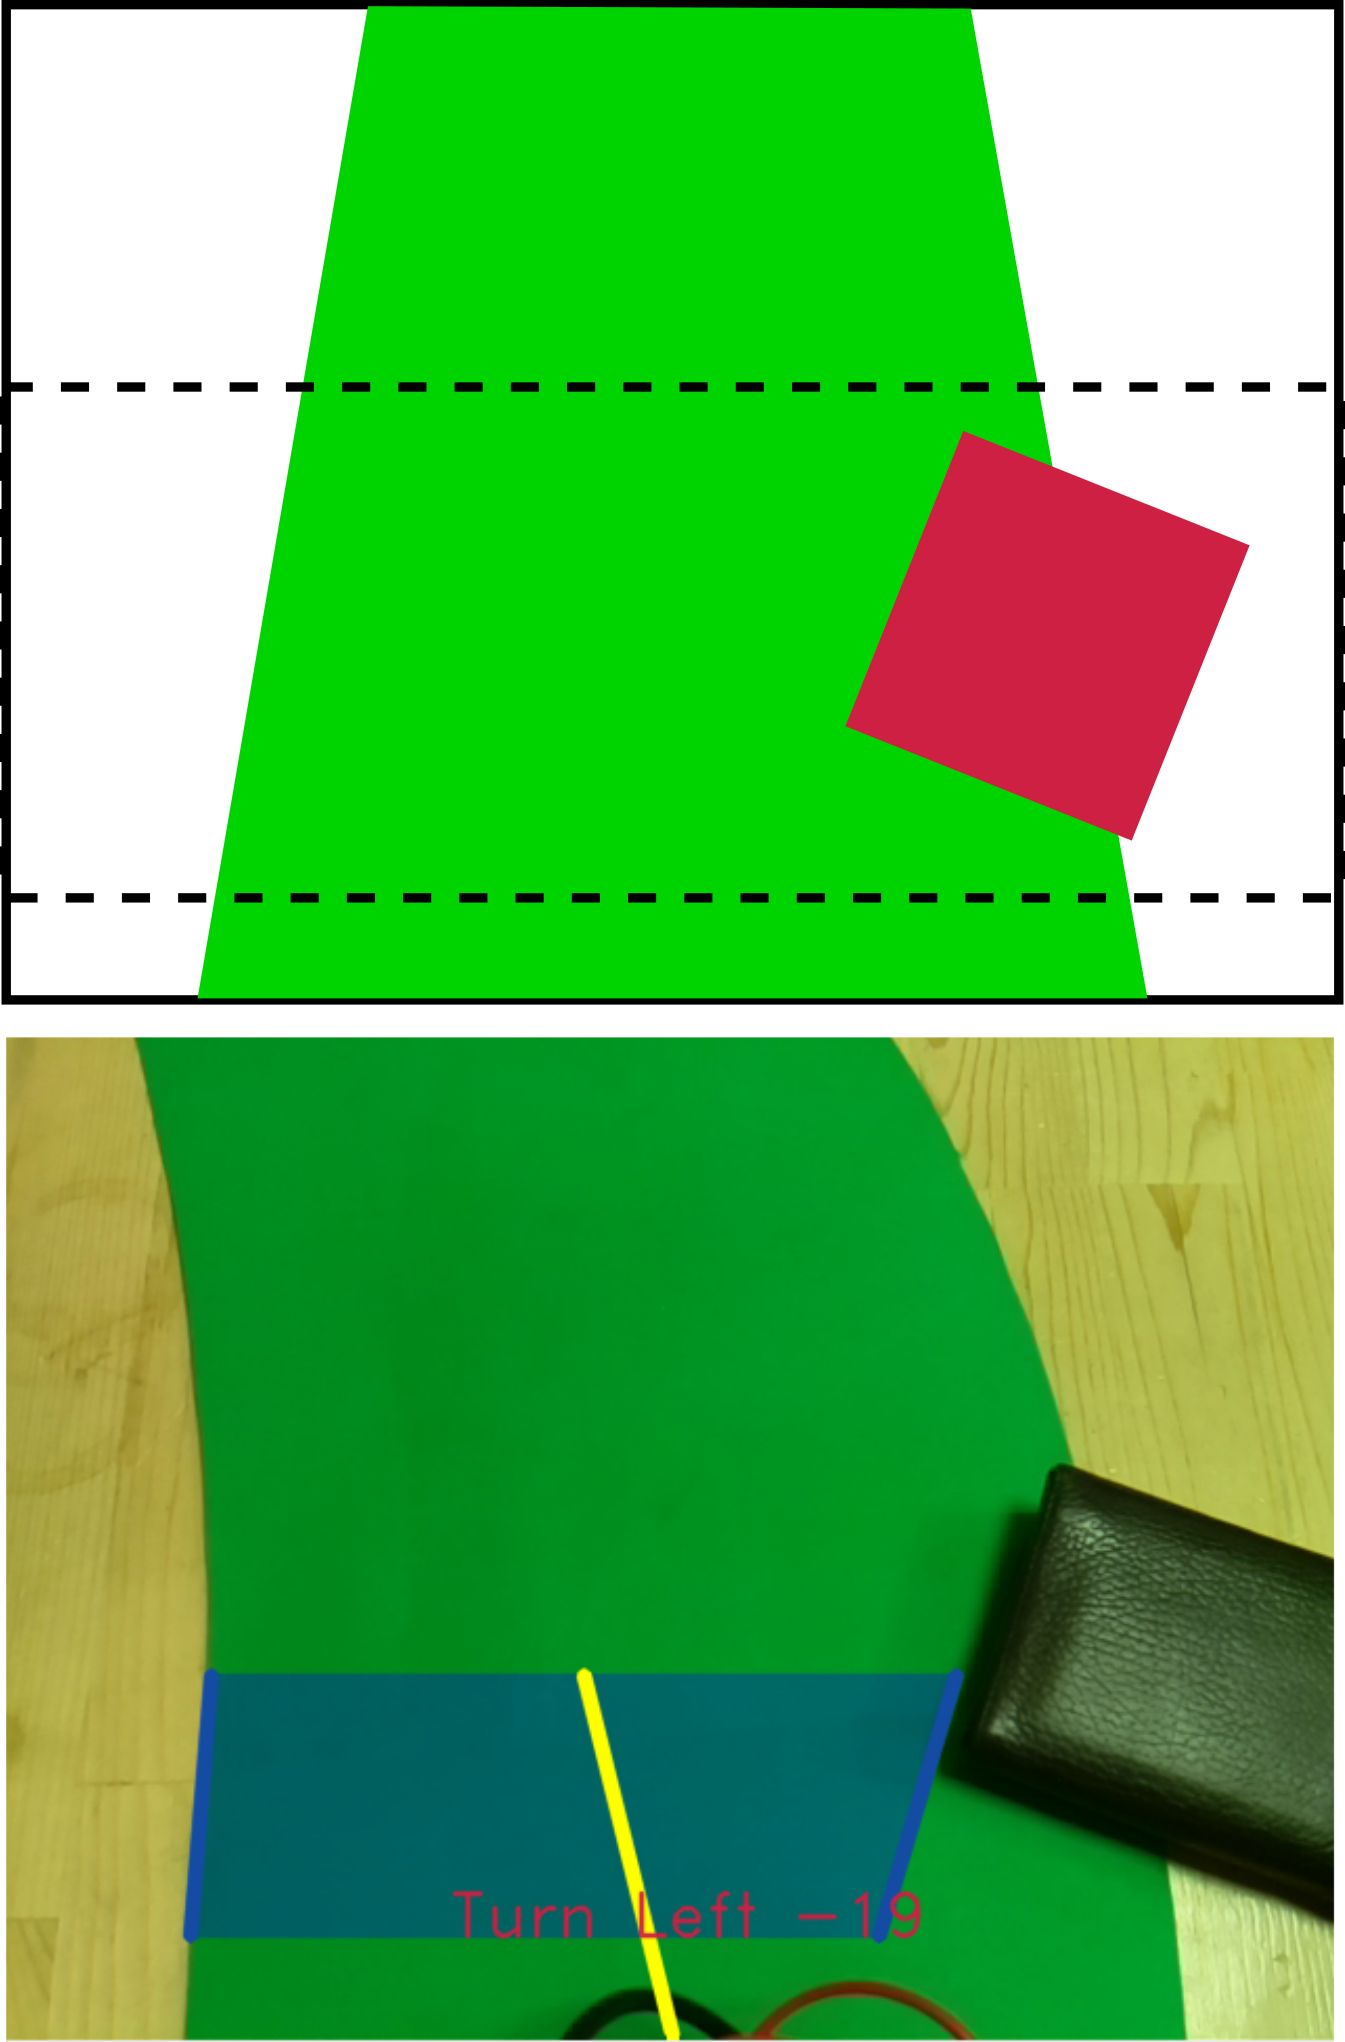
\includegraphics[width=0.30\unitlength]{images/path_images/up_2}
		\caption{\label{fig:dataP_up_2} Obstacle is at the Middle of the Path}
	\end{subfigure}
		\begin{subfigure}{.31\textwidth}
		\centering
		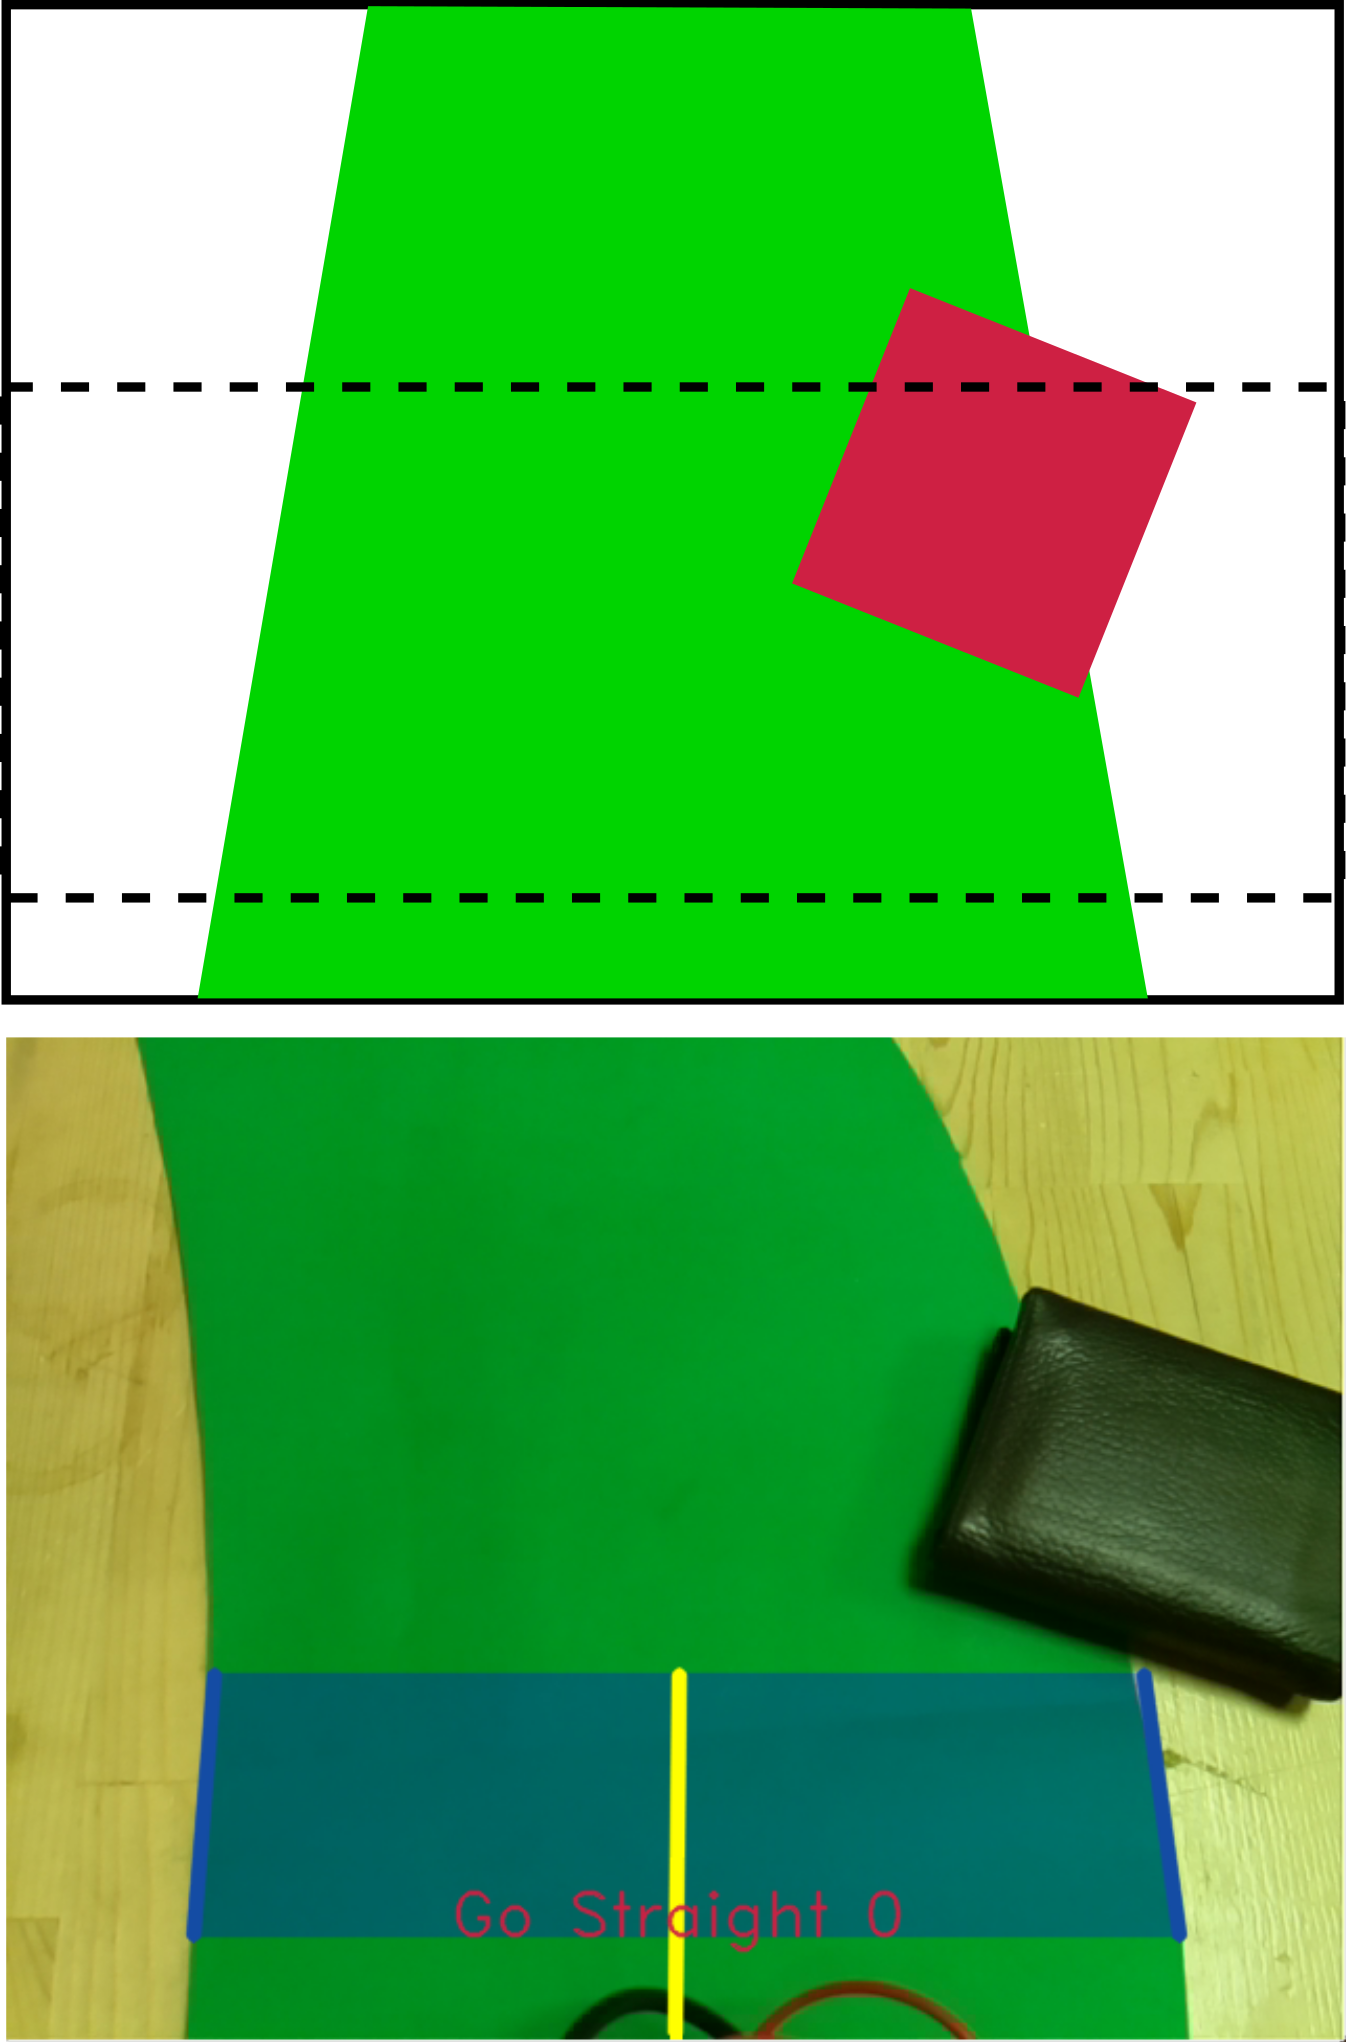
\includegraphics[width=0.30\unitlength]{images/path_images/up_3}
		\caption{\label{fig:dataP_up_3} Obstacle is at the End of the Path.}
	\end{subfigure}
	\caption{\label{fig:dataP_up} A Test Scenario: Upward Inclined Obstacle on the Path. \\ Upper Half: Proposed Tests, Lower Half: Results}
\end{figure}
	
	\begin{figure}[H]
	\setlength{\unitlength}{\textwidth} 
	\centering
	\begin{subfigure}{.31\textwidth}
		\centering
		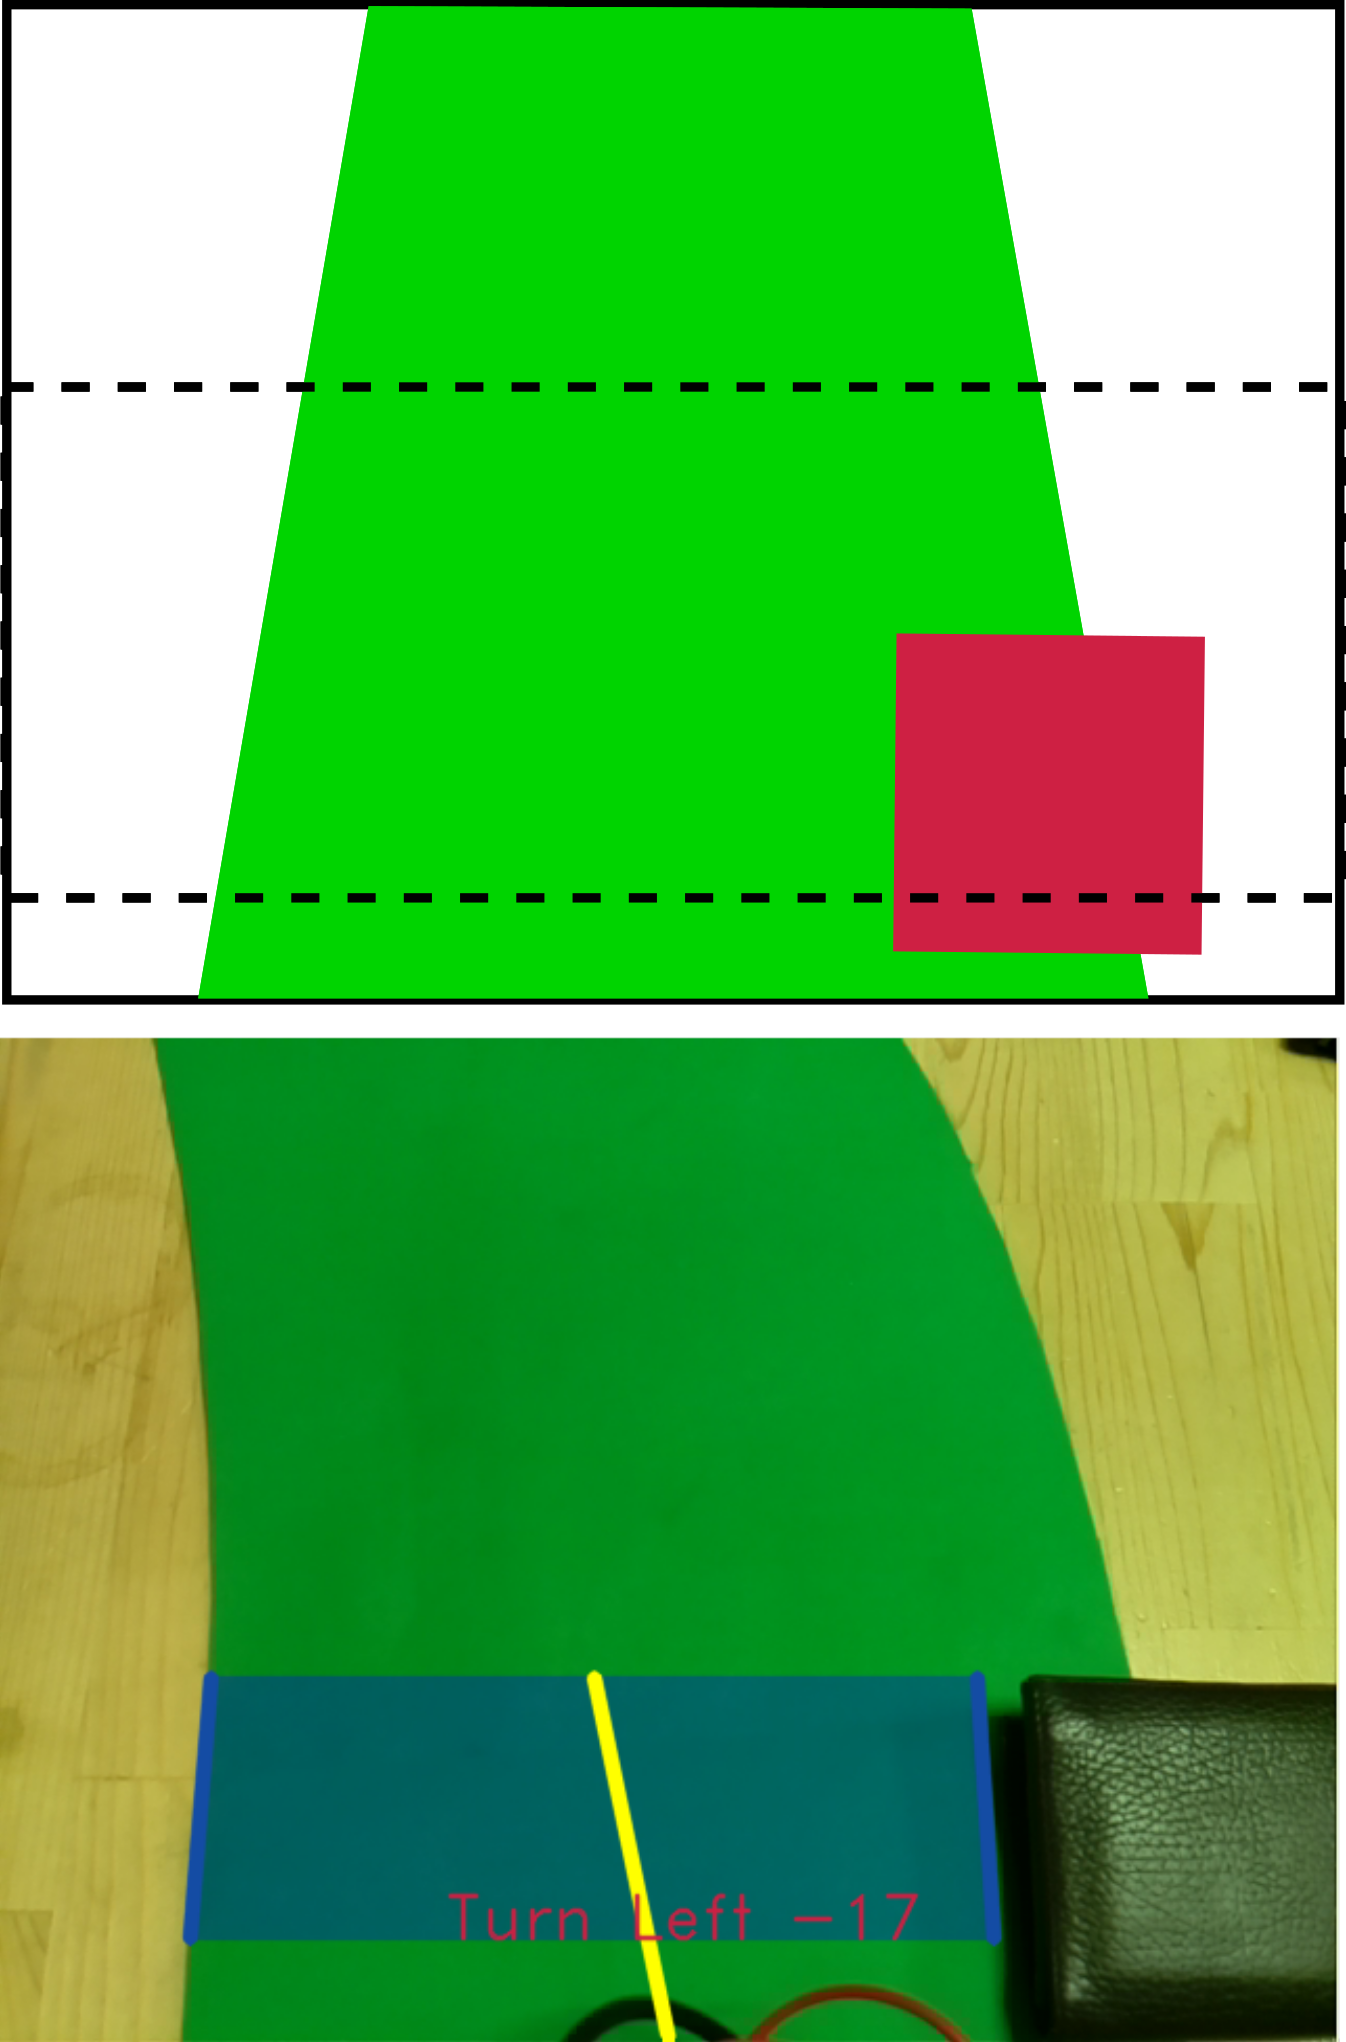
\includegraphics[width=0.30\unitlength]{images/path_images/par_1}
		\caption{\label{fig:dataP_par_1} Obstacle is at the Beginning of the Path}
	\end{subfigure}%
	\begin{subfigure}{.31\textwidth}
		\centering
		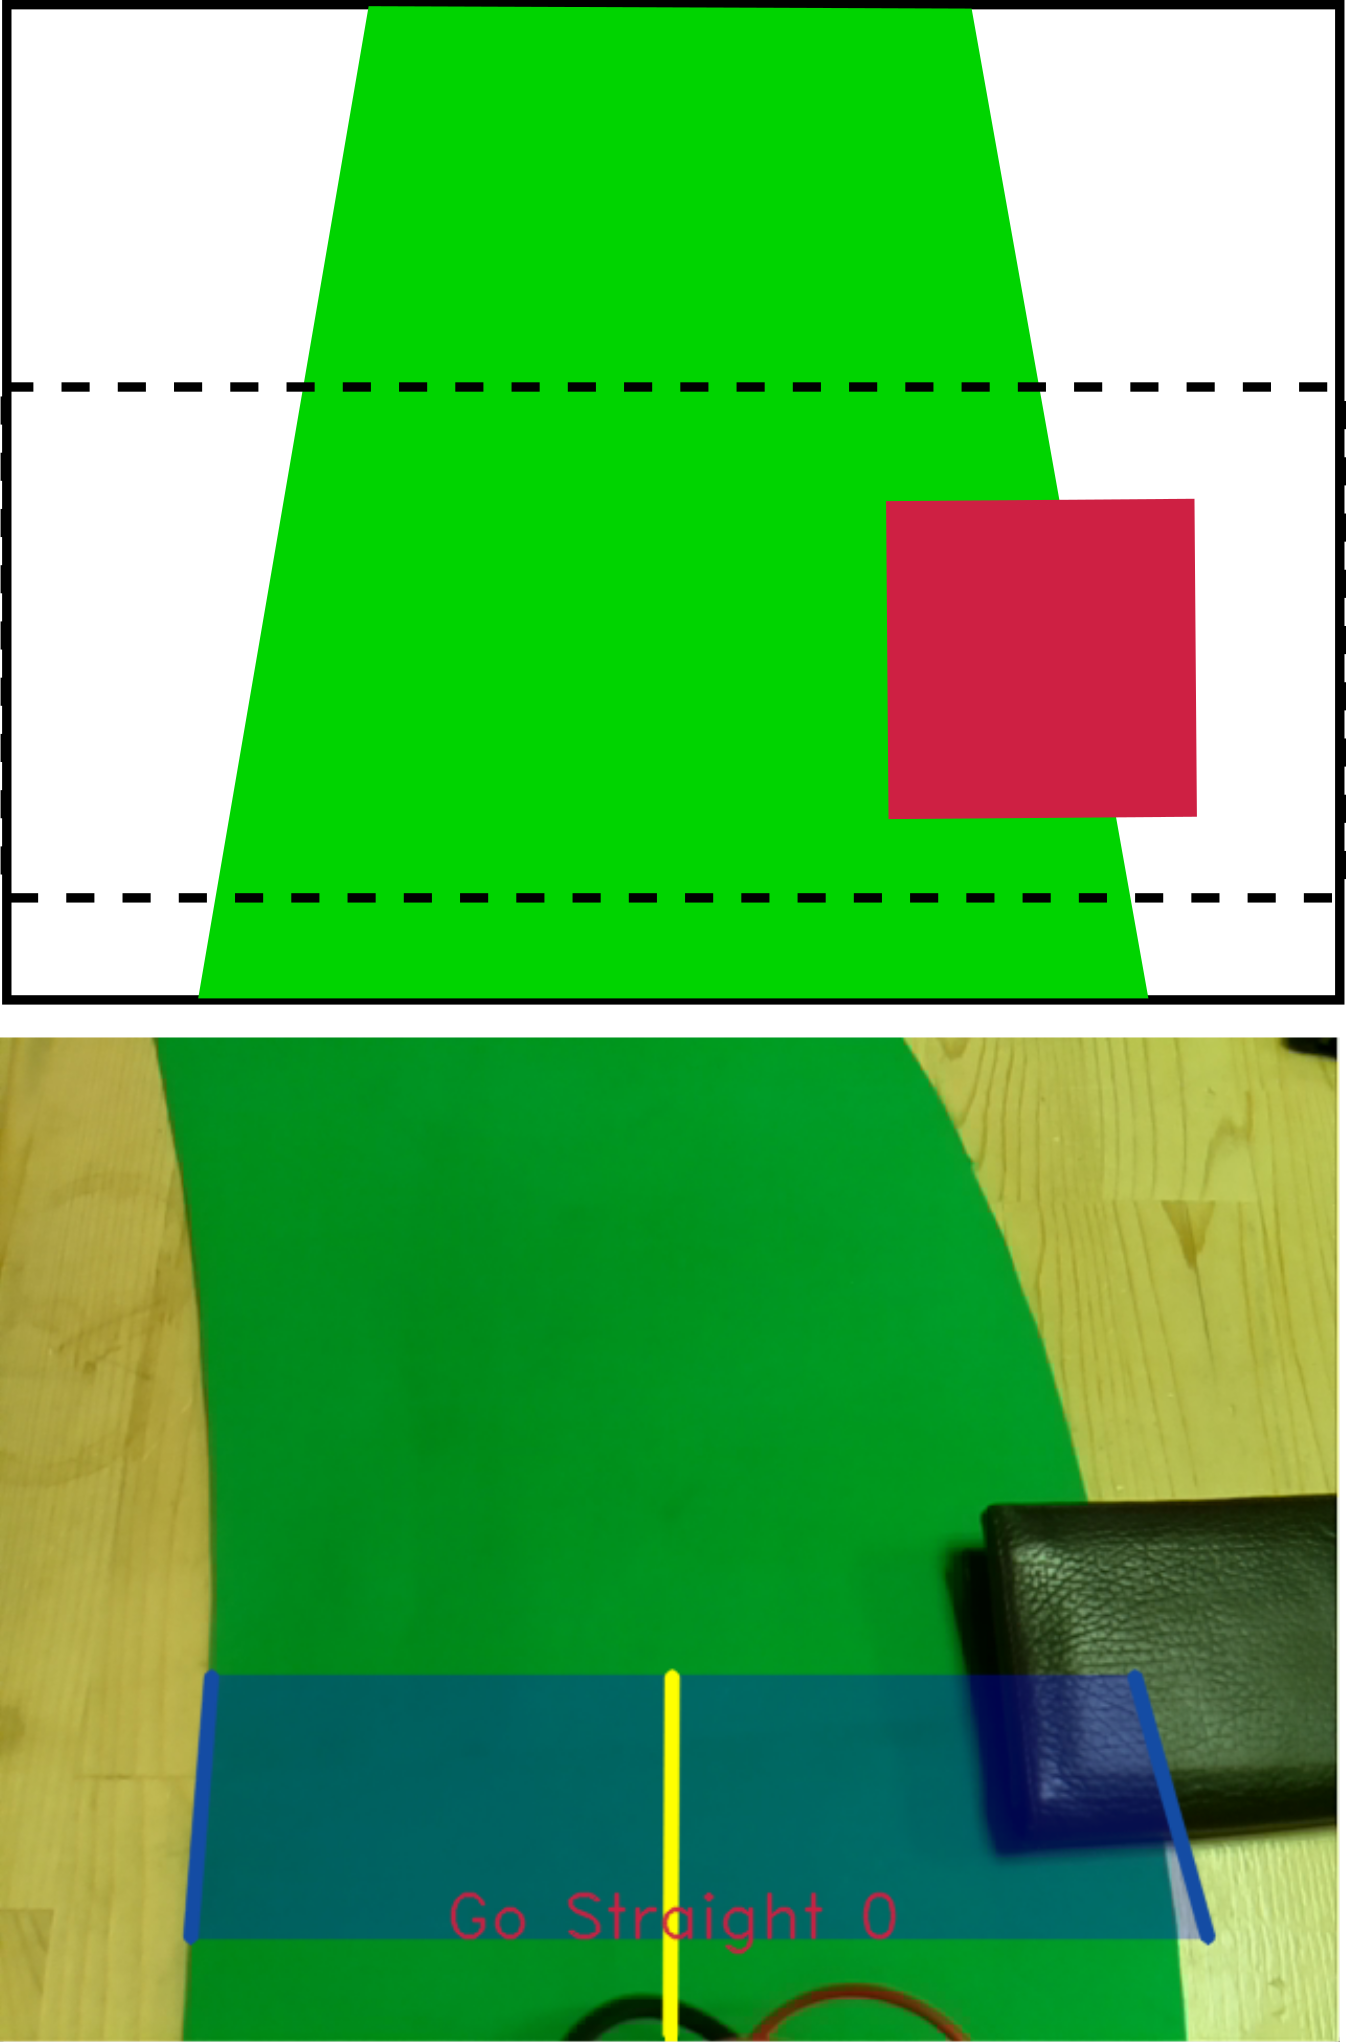
\includegraphics[width=0.30\unitlength]{images/path_images/par_2}
		\caption{\label{fig:dataP_par_2} Obstacle is at the Middle of the Path}
	\end{subfigure}
		\begin{subfigure}{.31\textwidth}
		\centering
		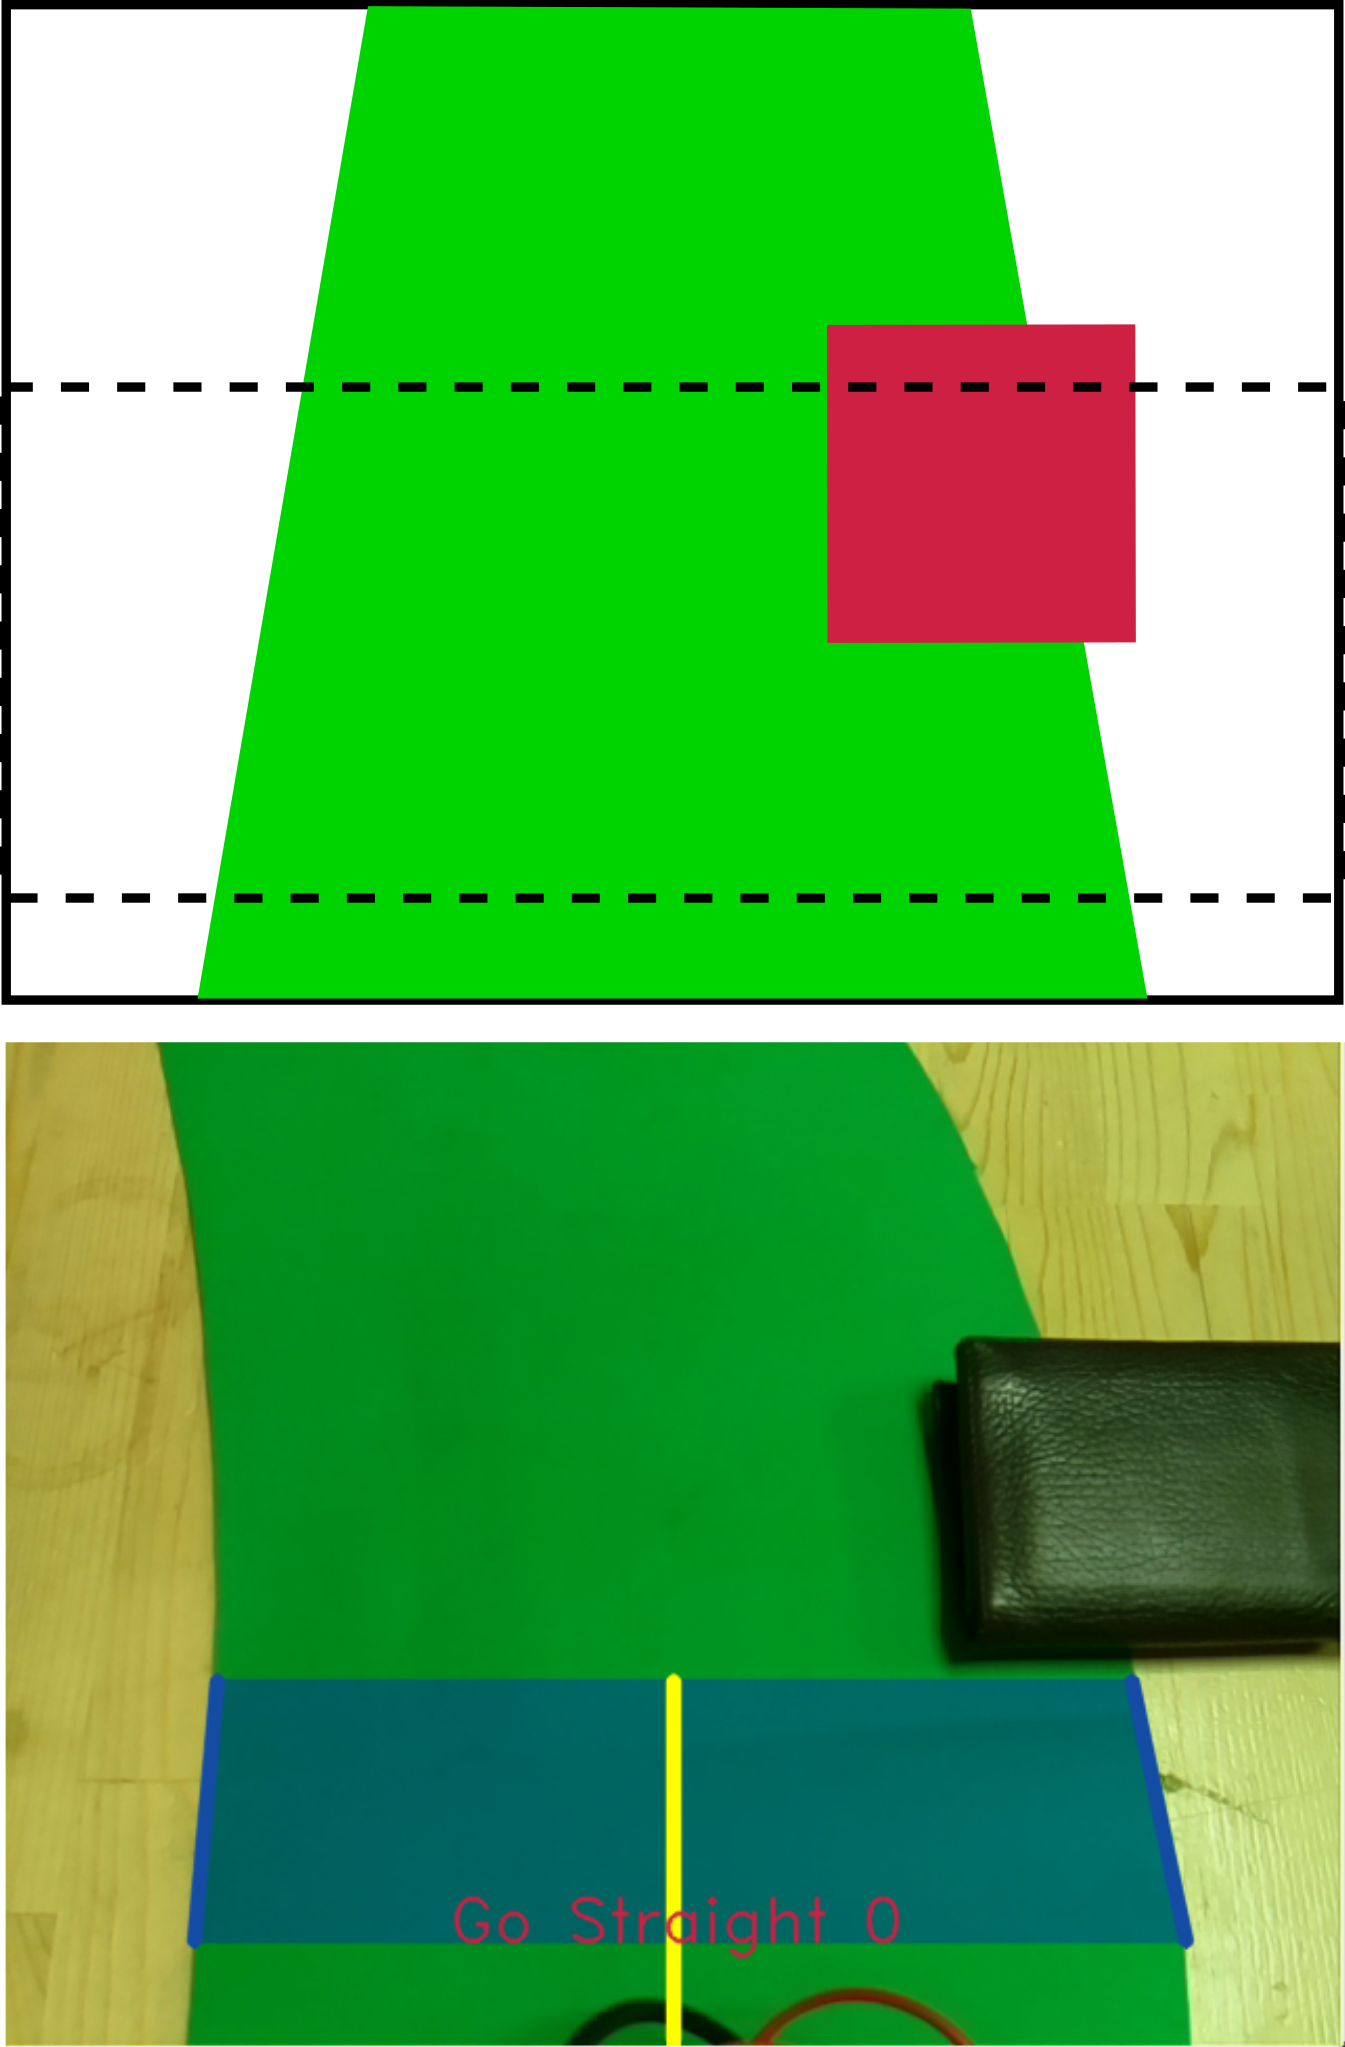
\includegraphics[width=0.30\unitlength]{images/path_images/par_3}
		\caption{\label{fig:dataP_par_3} Obstacle is at the End of the Path.}
	\end{subfigure}
	\caption{\label{fig:dataP_par} A Test Scenario: Parallel Placed Obstacle on the Path. \\ Upper Half: Proposed Tests, Lower Half: Results}
\end{figure}		

	\begin{figure}[H]
	\setlength{\unitlength}{\textwidth} 
	\centering
	\begin{subfigure}{.31\textwidth}
		\centering
		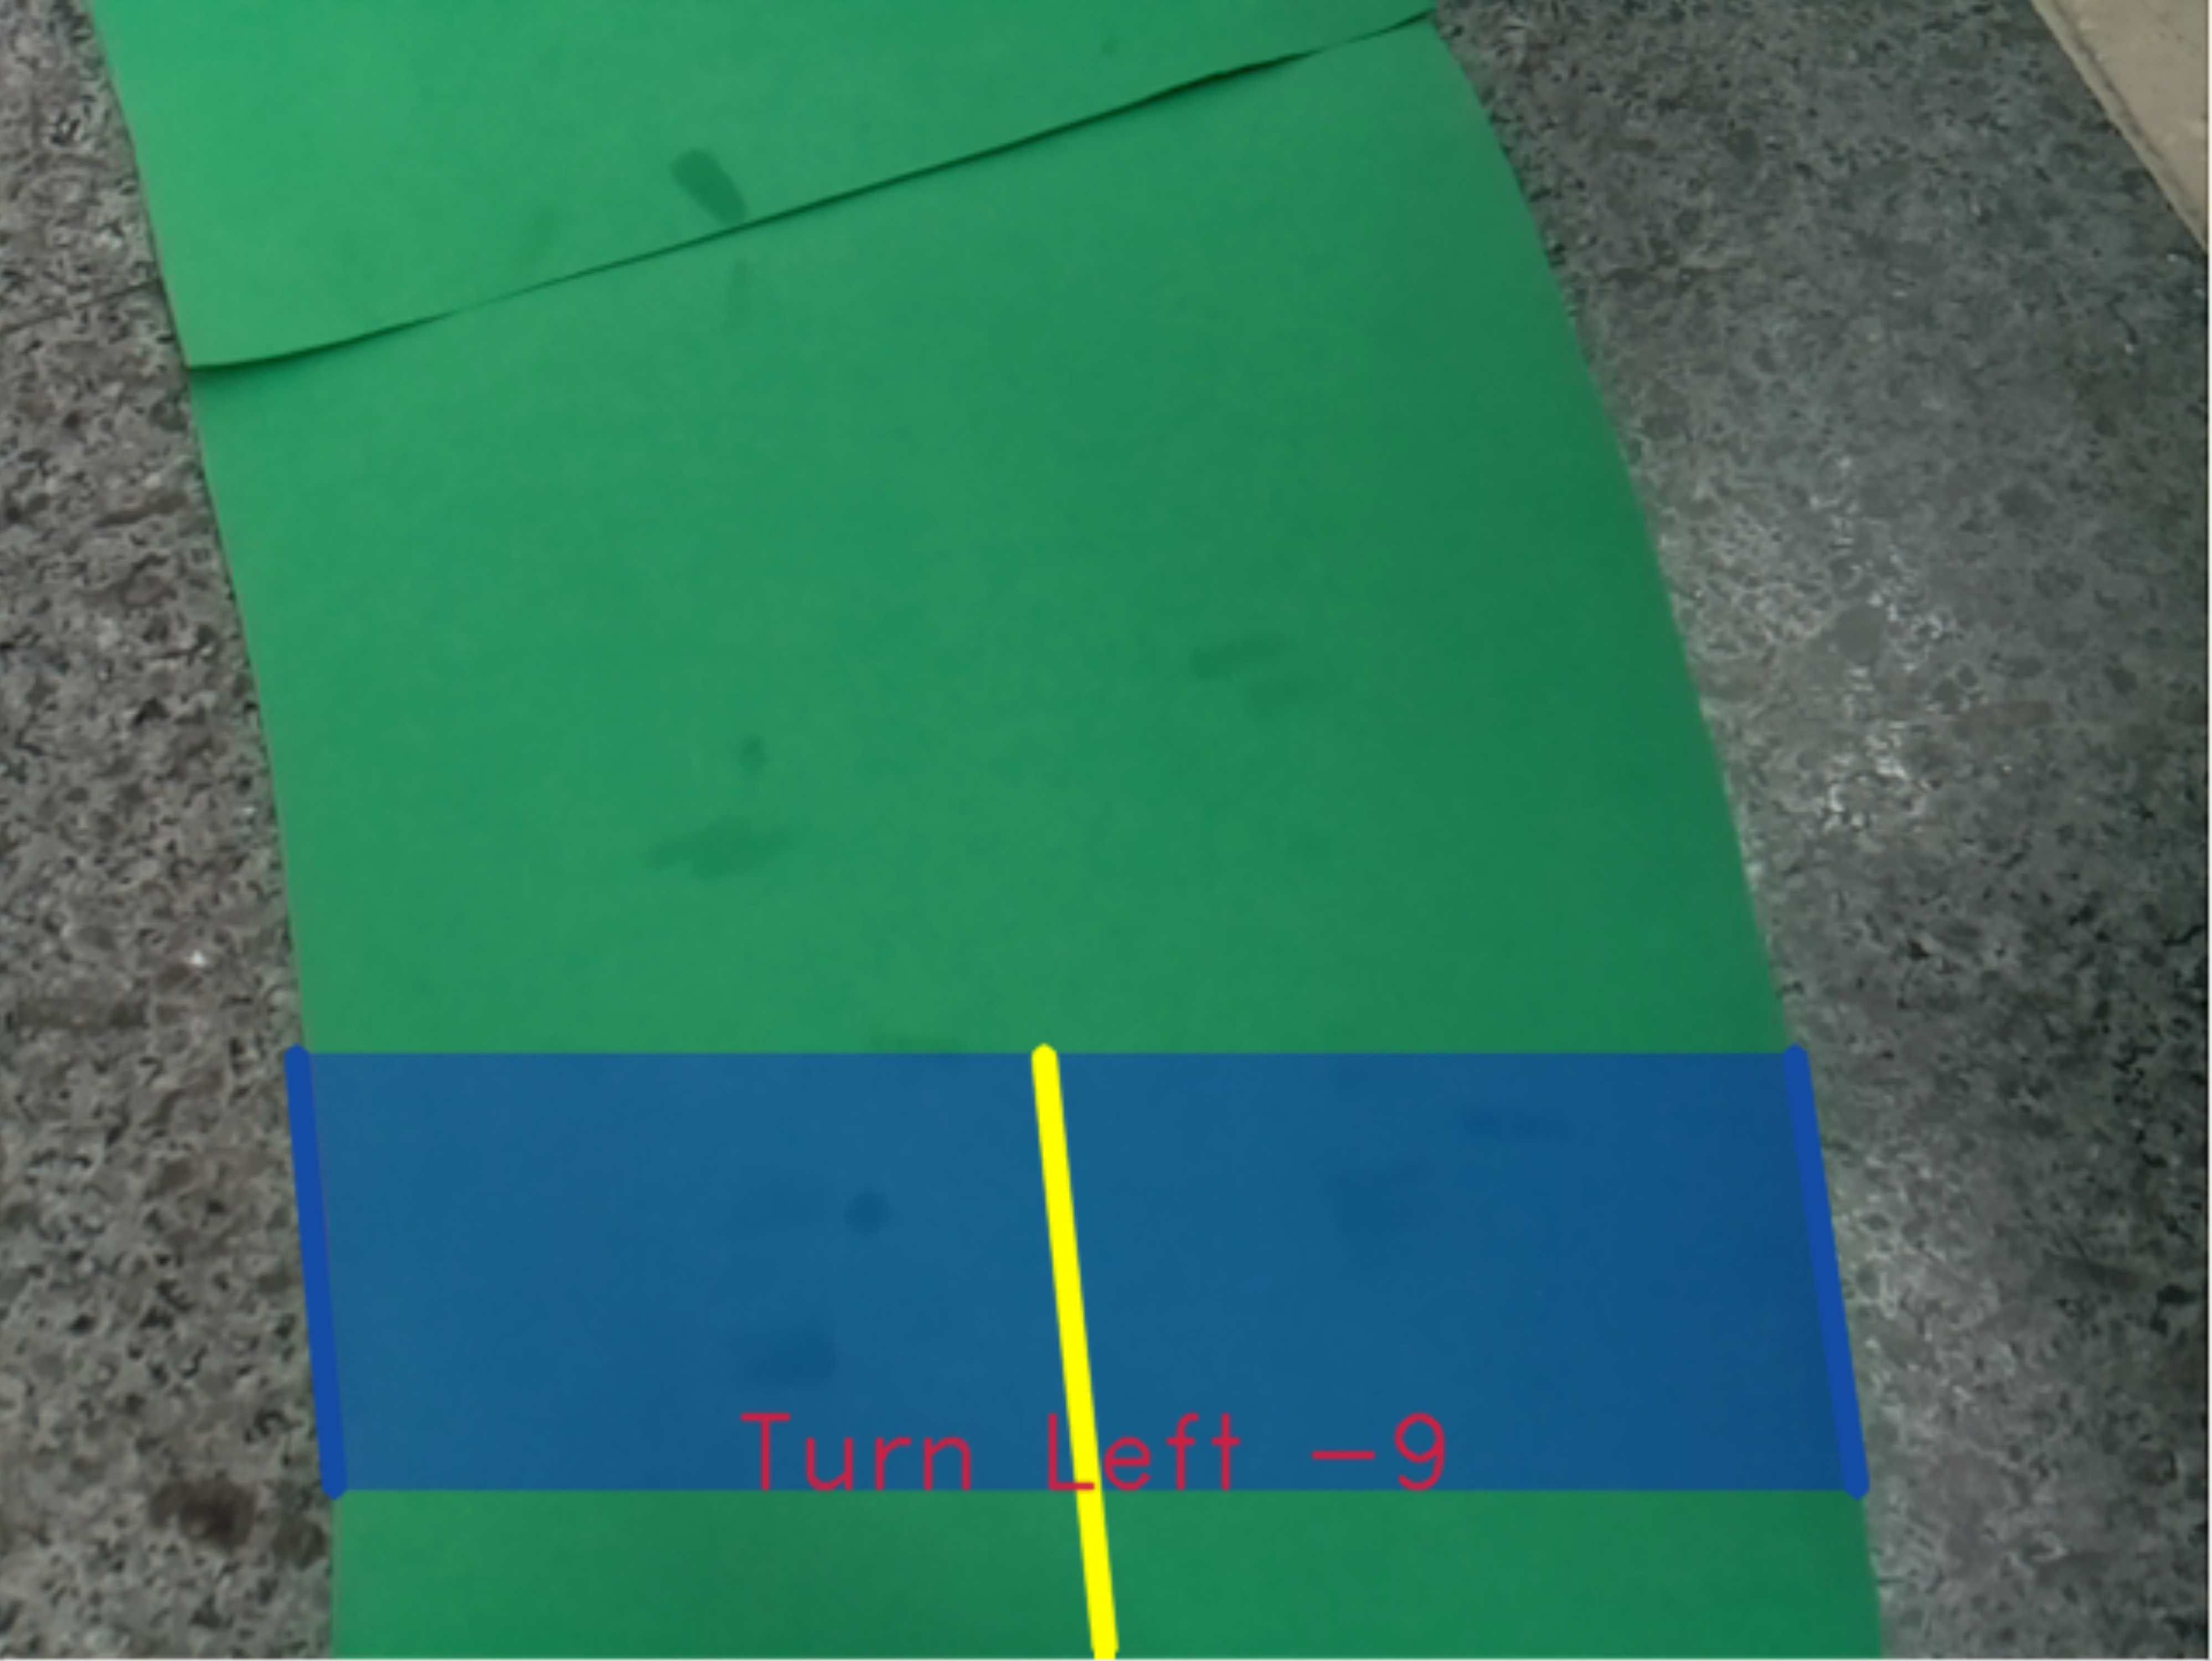
\includegraphics[width=0.30\unitlength]{images/path_images/inside-bb}
		\caption{\label{fig:dataP_inside-bb} Path is Placed on Black Marble}
	\end{subfigure}%
	\begin{subfigure}{.31\textwidth}
		\centering
		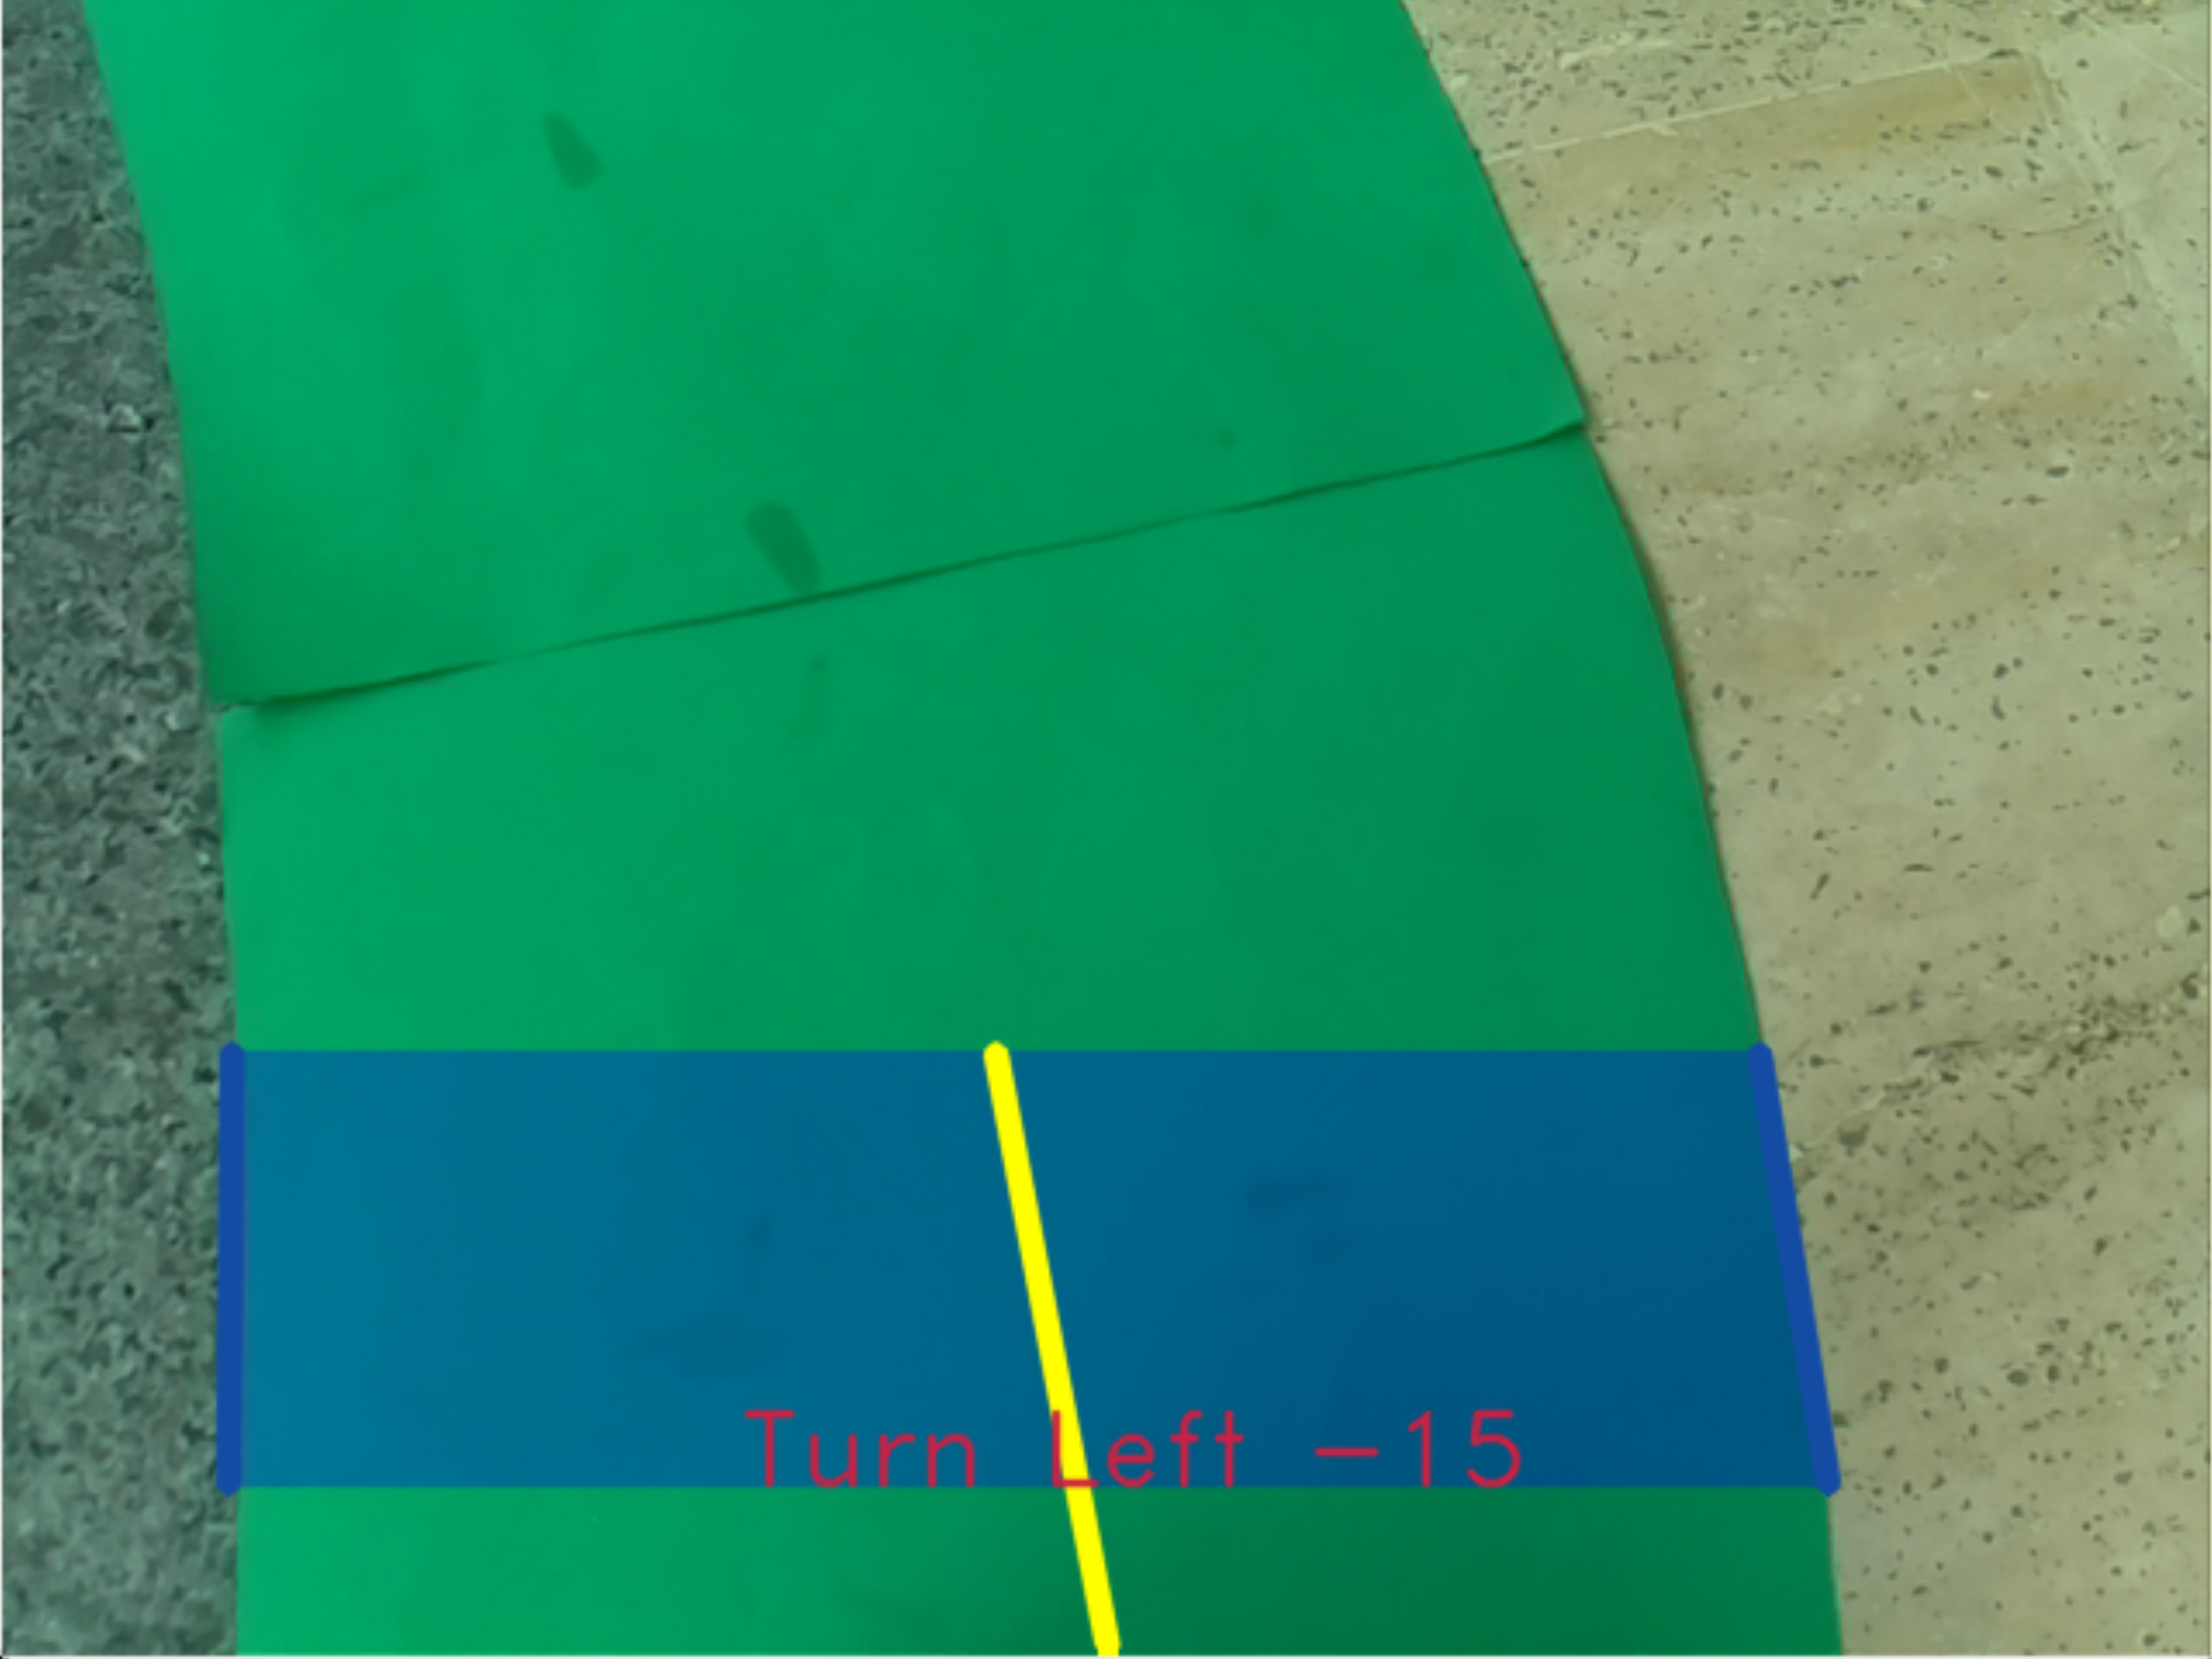
\includegraphics[width=0.30\unitlength]{images/path_images/inside-bw}
		\caption{\label{fig:dataP_inside-bw} Path is Placed on Black and White Marble}
	\end{subfigure}
		\begin{subfigure}{.31\textwidth}
		\centering
		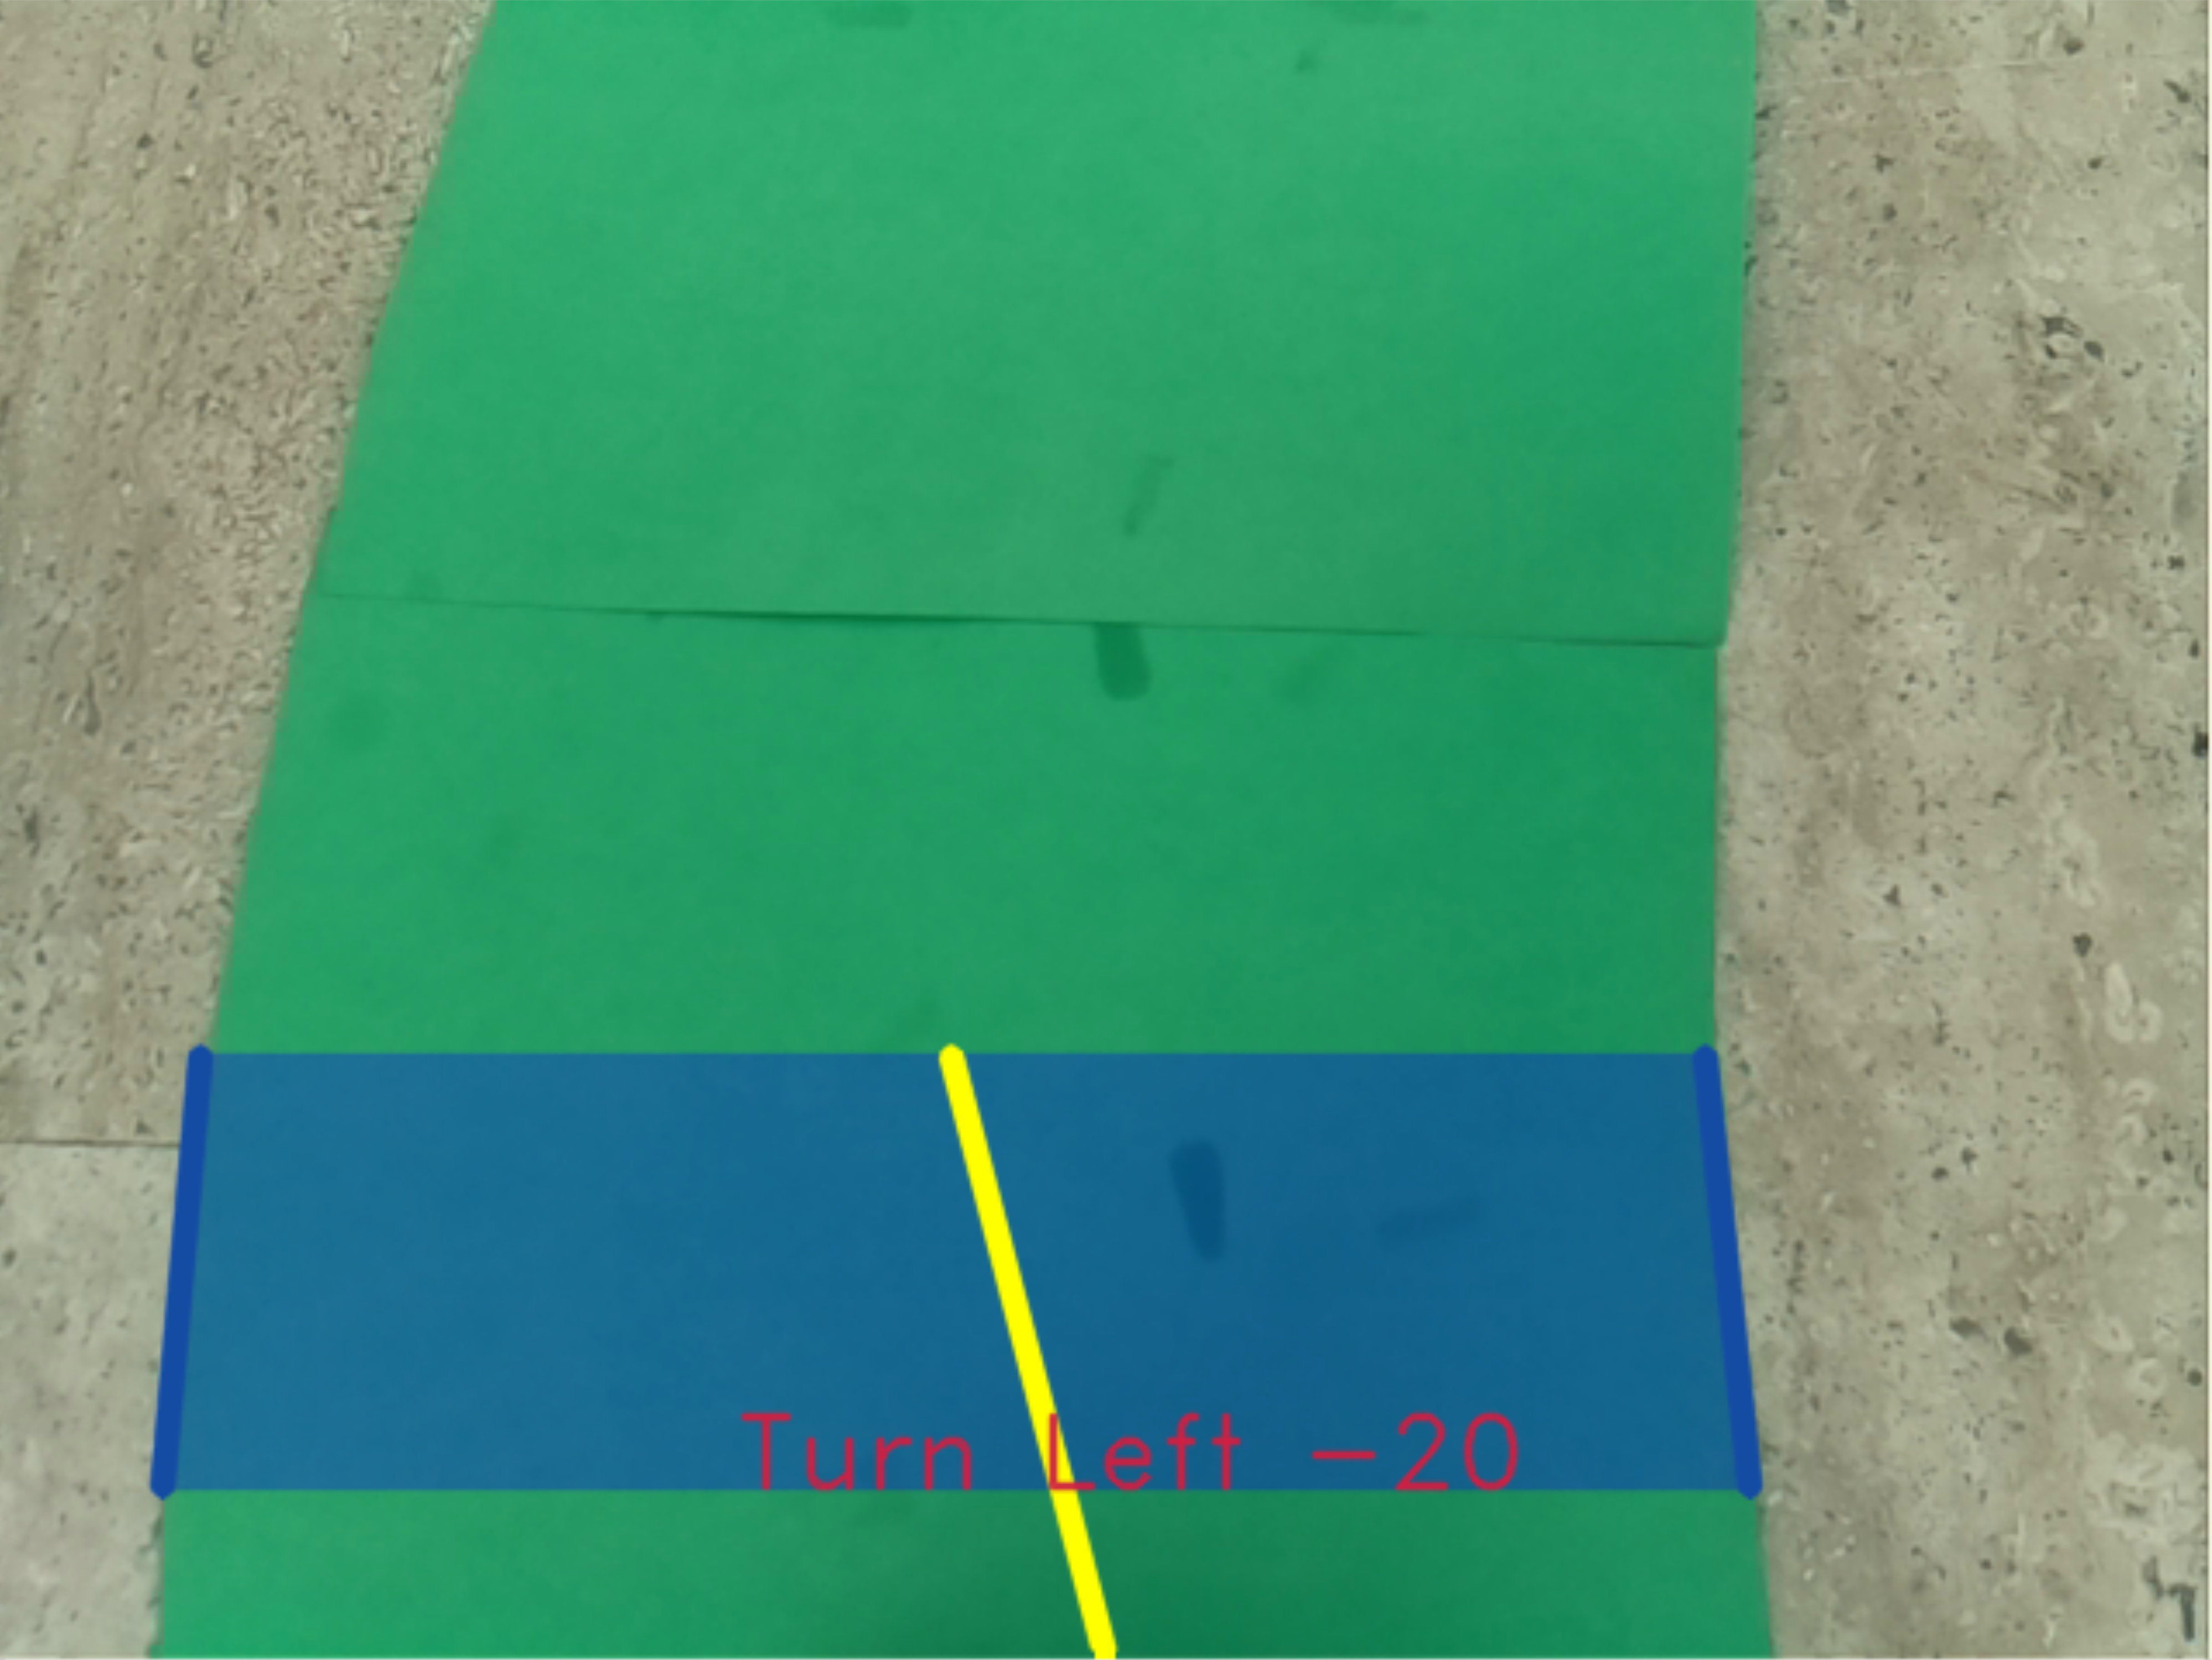
\includegraphics[width=0.30\unitlength]{images/path_images/inside-ww}
		\caption{\label{fig:dataP_inside-ww} Path is Placed on White Marble}
	\end{subfigure}
	\caption{\label{fig:dataP_inside} A Test Scenario Results: KKM Indoor Path Detection}
\end{figure}

	\begin{figure}[H]
	\setlength{\unitlength}{\textwidth} 
	\centering
	\begin{subfigure}{.31\textwidth}
		\centering
		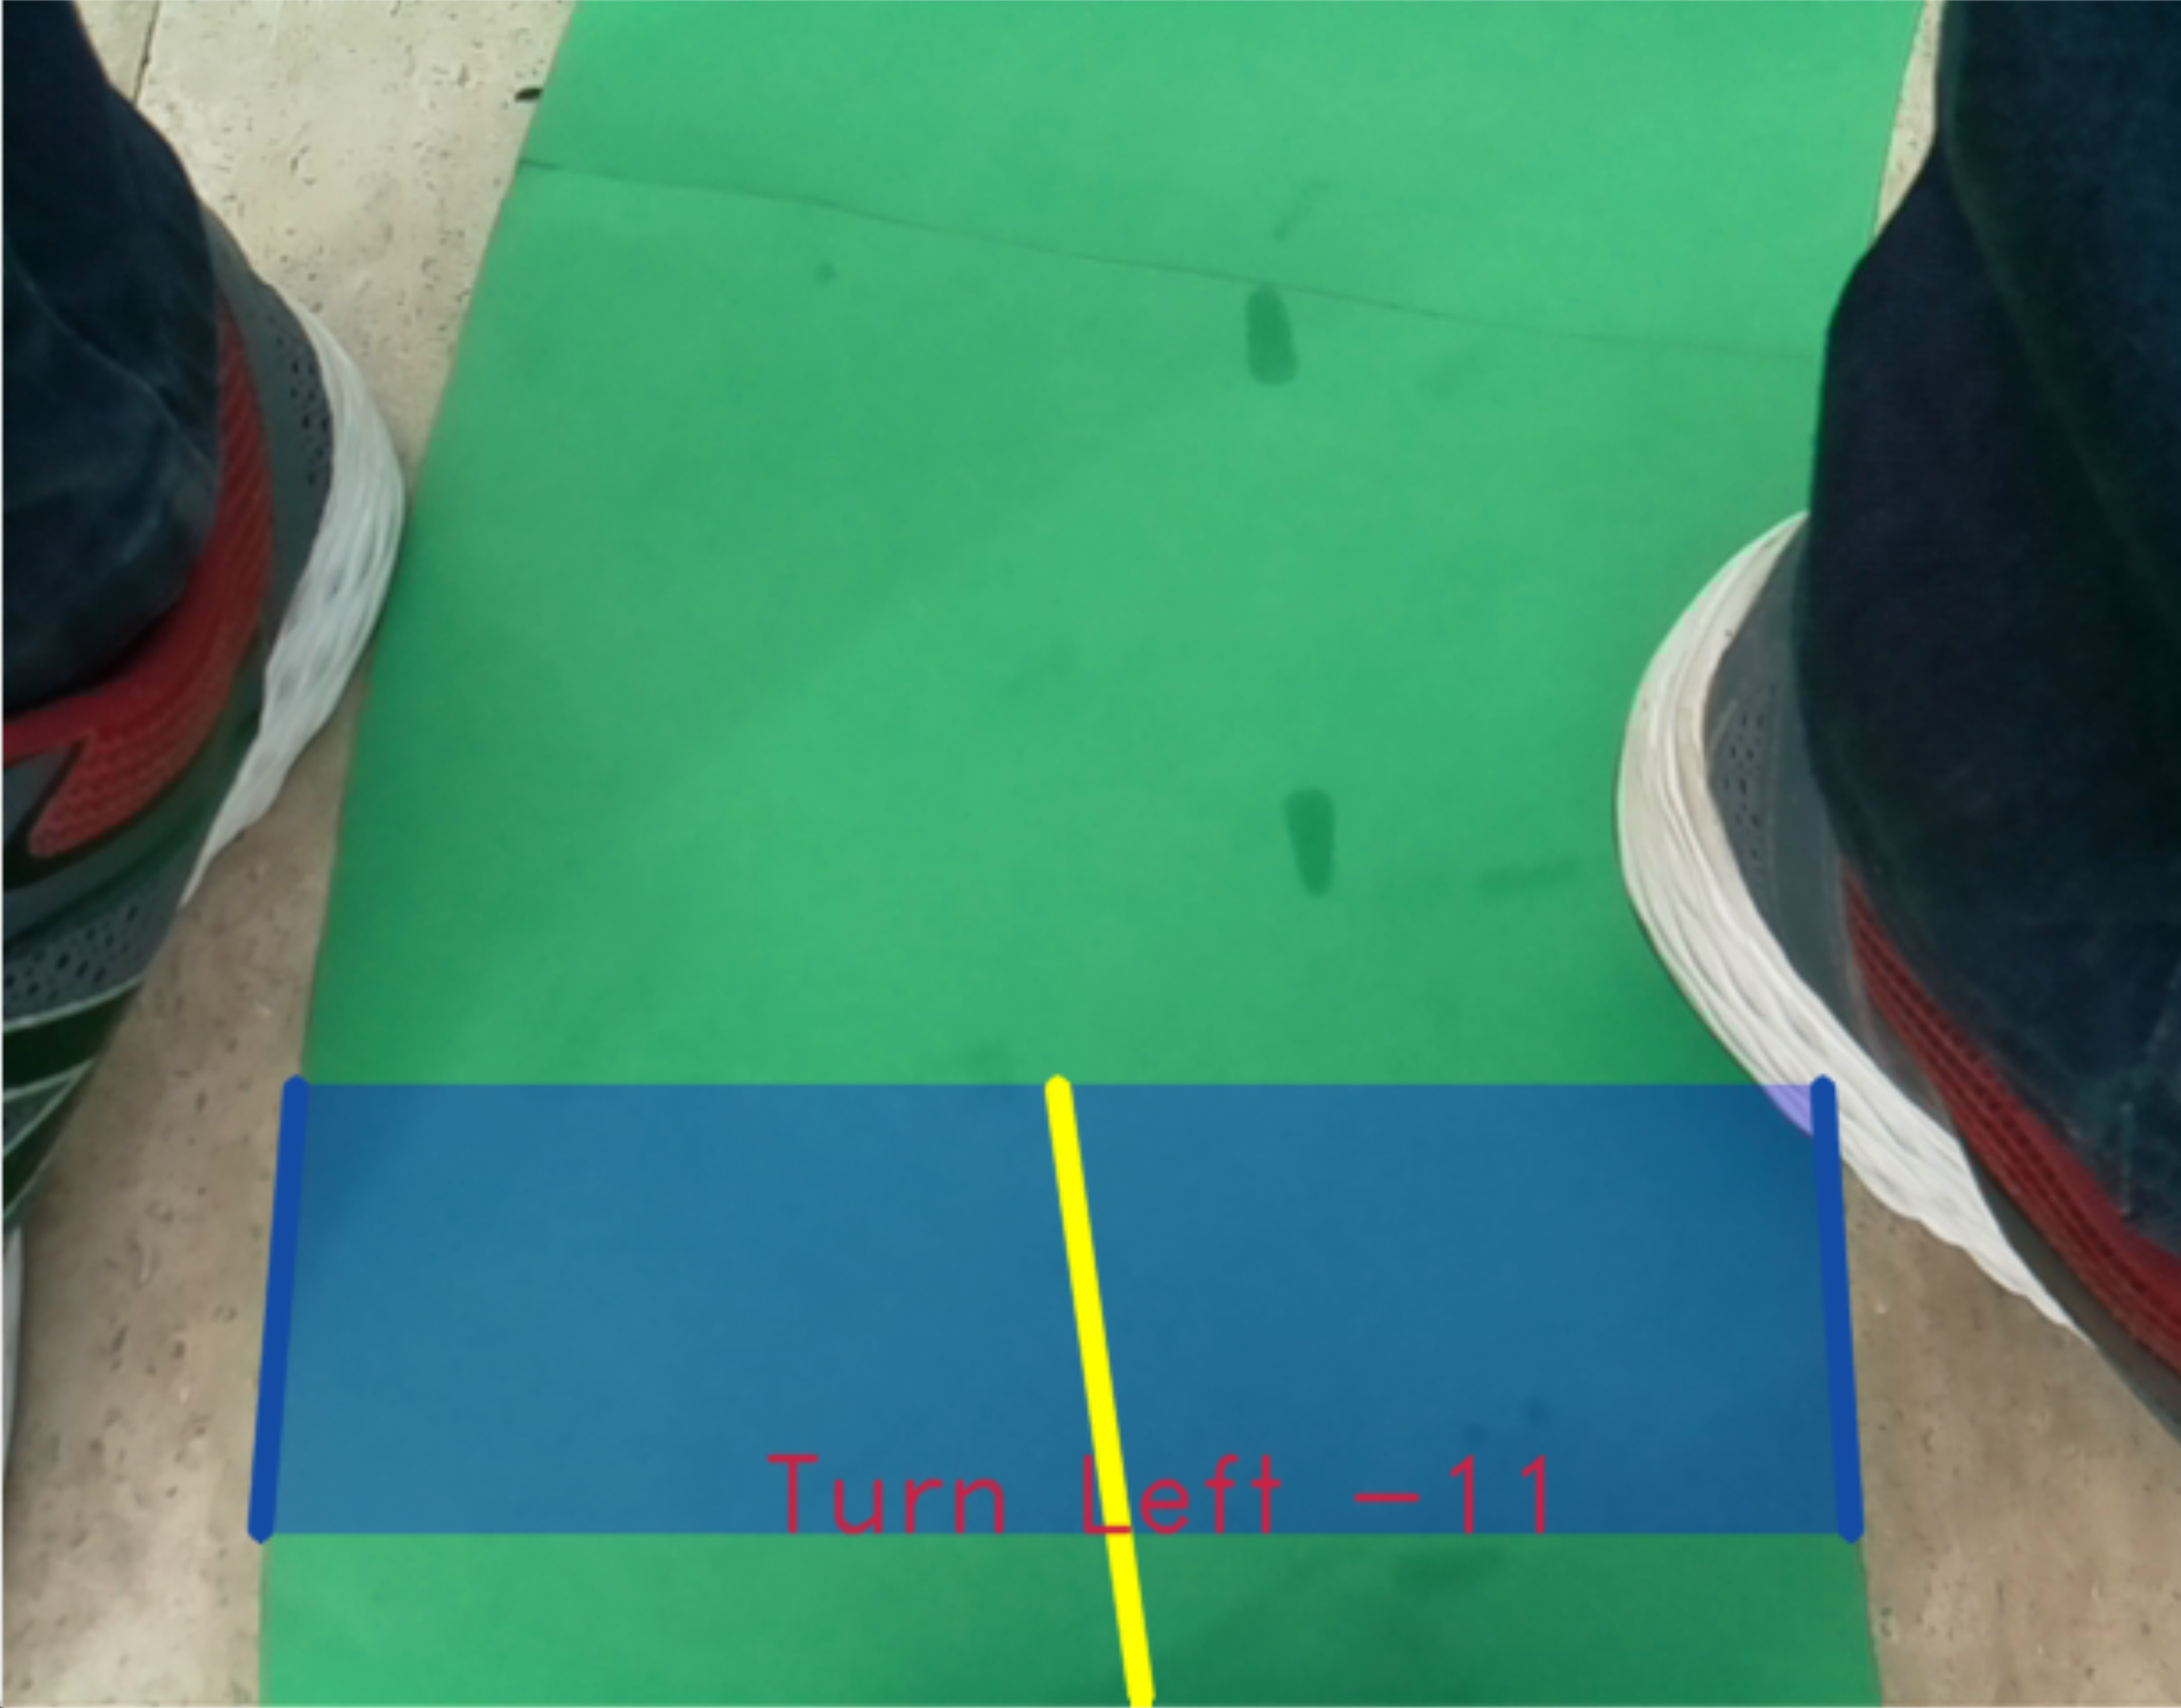
\includegraphics[width=0.30\unitlength]{images/path_images/outsideObs0}
		\caption{\label{fig:dataP_outsideObs0} Daylight and Shadow Test-1}
	\end{subfigure}%
	\begin{subfigure}{.31\textwidth}
		\centering
		\includegraphics[width=0.30\unitlength]{images/path_images/outsideObs1}
		\caption{\label{fig:dataP_outsideObs1} Daylight and Shadow Test-2}
	\end{subfigure}
		\begin{subfigure}{.31\textwidth}
		\centering
		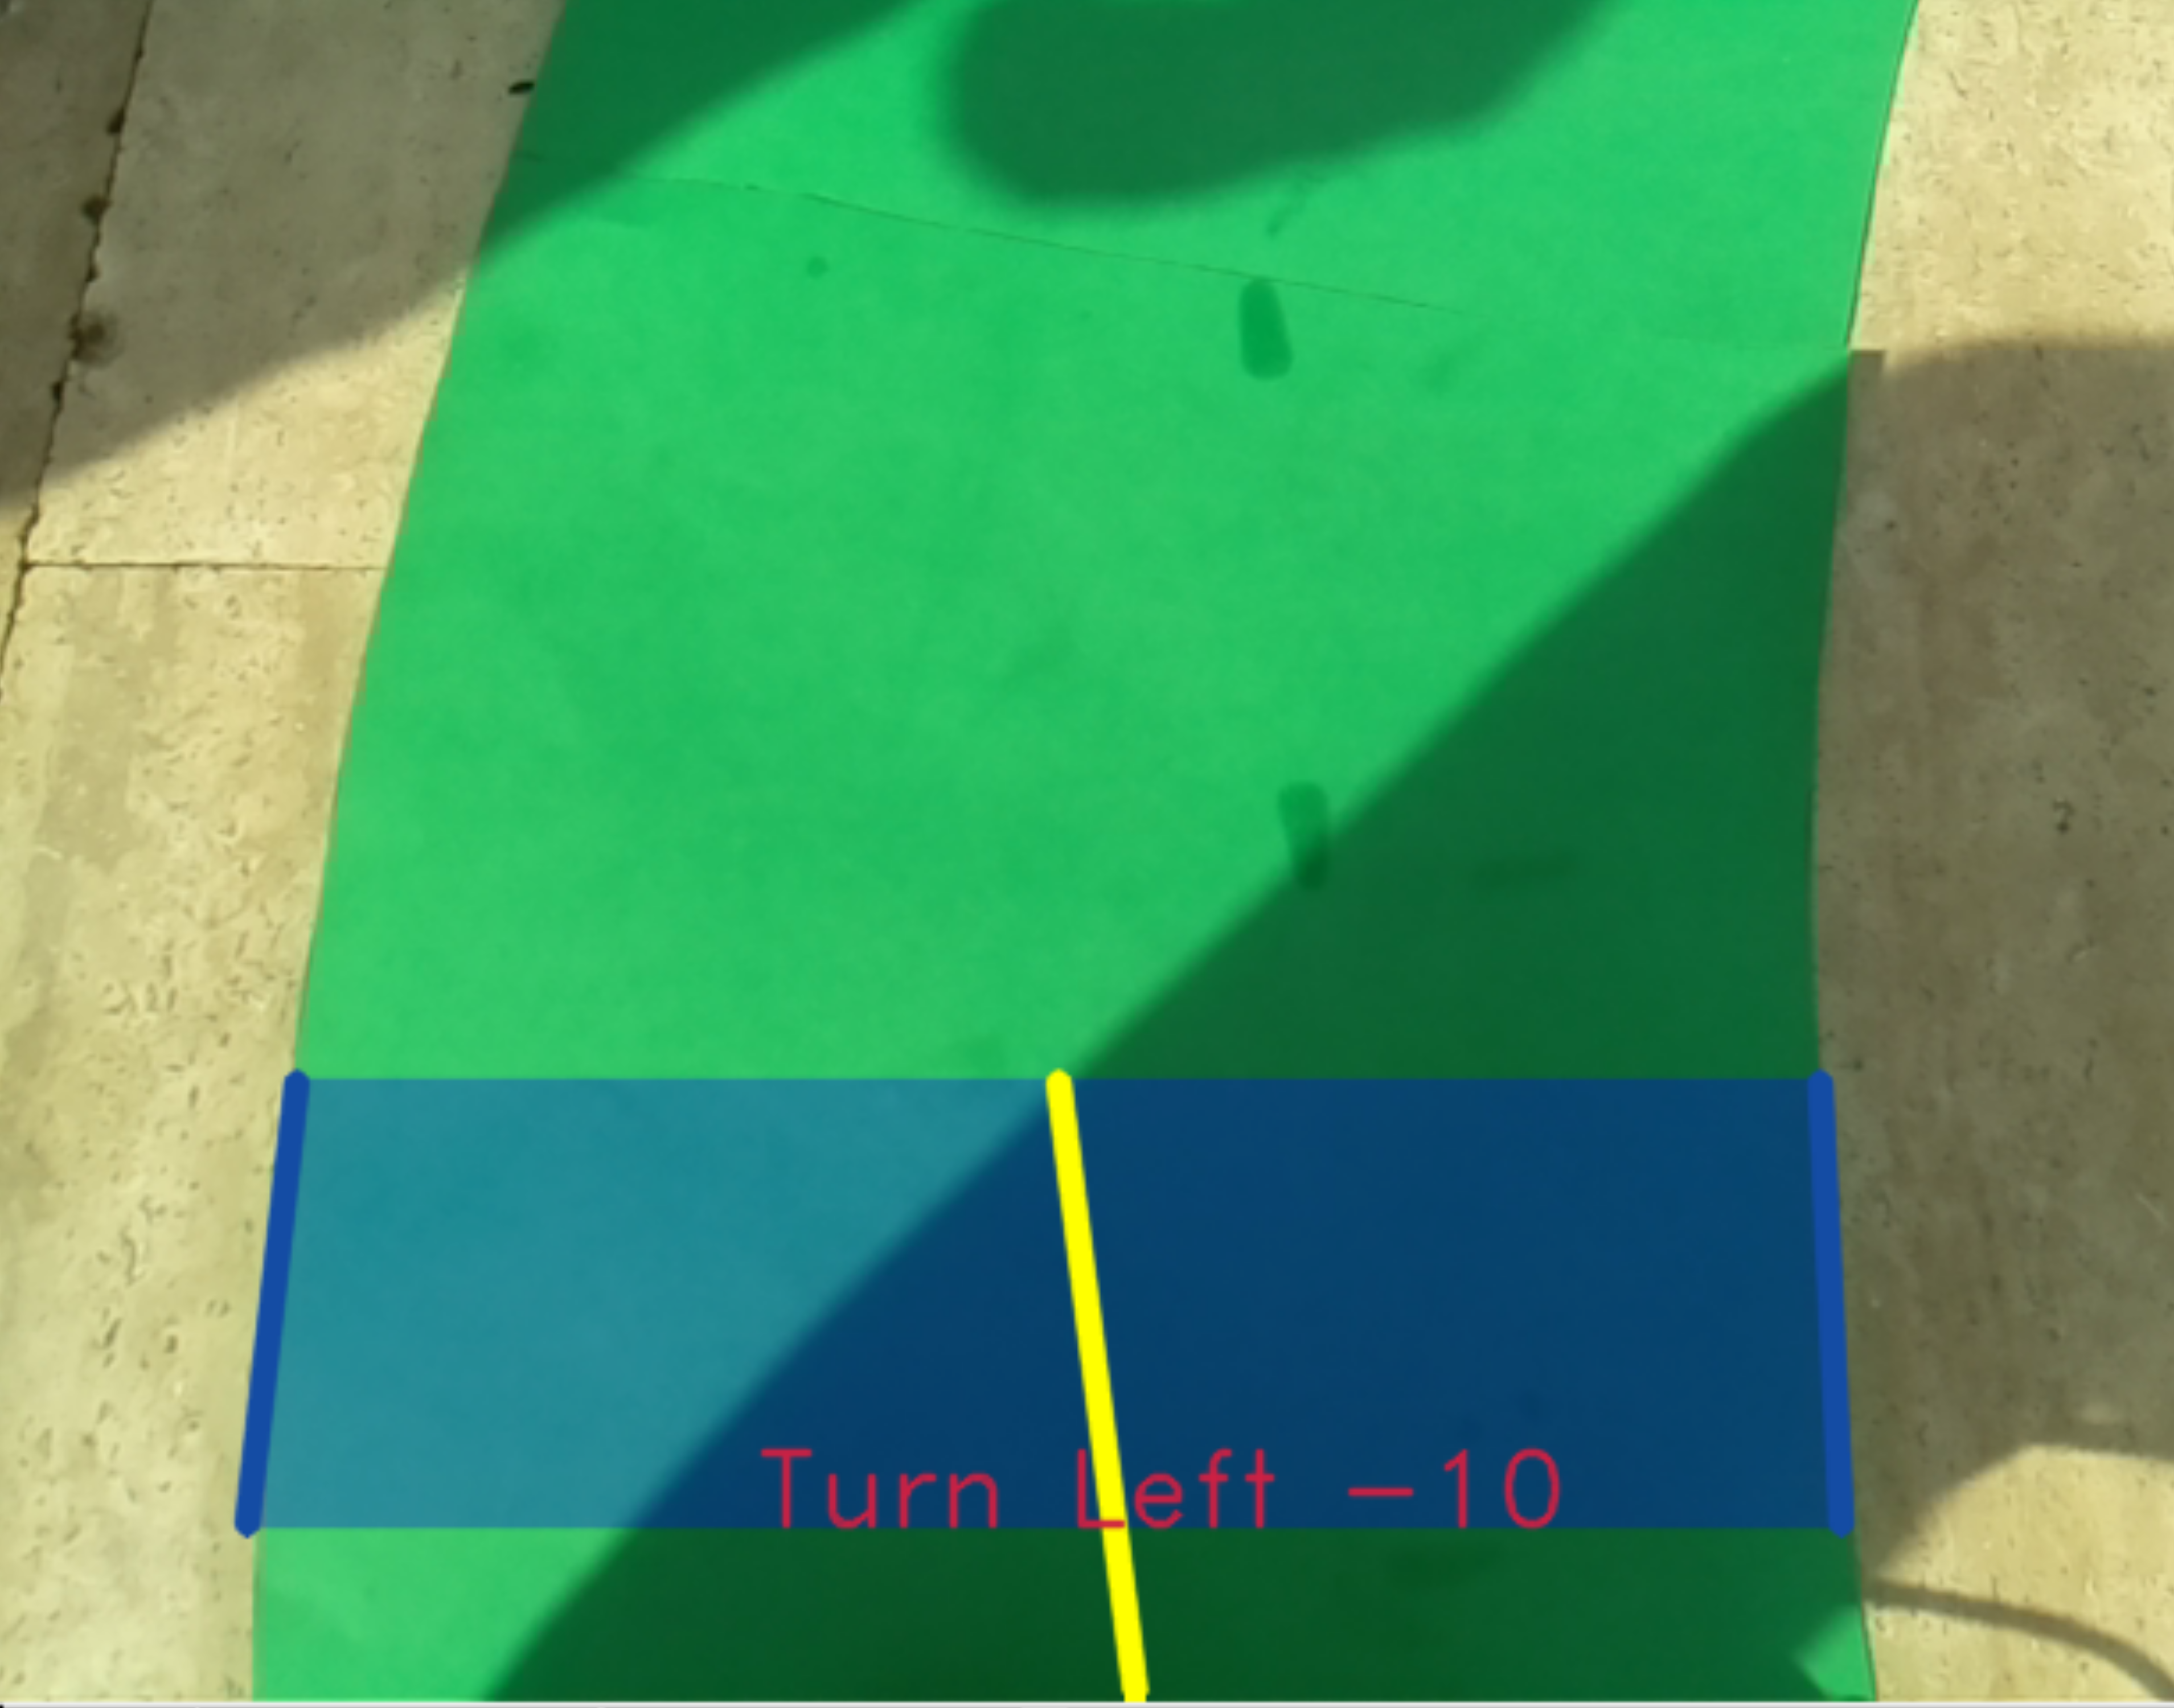
\includegraphics[width=0.30\unitlength]{images/path_images/outsideObs2}
		\caption{\label{fig:dataP_outsideObs2} Daylight and Shadow Test-3}
	\end{subfigure}
	\caption{\label{fig:dataP_outside} A Test Scenario Results: KKM Outdoor Path Detection}
\end{figure}	
		
		
	\subsubsection*{Results of PID Controller Subsystem Tests}
	
		Due to other limitations, the initial version of the PID controller subsystem was tested only for \textit{PID Parameters Test for Given Input}. The test results were promising for the time being. Other tests are planning to be conducted on the subsystem in the following semester.
	
	
	
	
	
	
	
	\subsubsection*{Results of Internal Communication Subsystem Tests}
	The results of the tests revealed that all steps are successful but the last step. The data send rate is determined to be 25 strings per second. The string length varies between one and three characters. The data is fully received if the rate is slower than 25 strings per second. However, the data loss  and  improper decoding is observed on the Arduino side. This must corrected by means of coding or switching to an alternative solution.
	

	
	
	
		

	\subsubsection*{Results of External Communication Subsystem Tests}
	
	 The first and simplest test has been done on one computer (or raspberry pi) using the same device as client and server, at the same time. To achieve that, the computer's (or raspberry pi’s) IP address should be defined in the host section defined in the client mode function. Secondly, the codes were tested on two computers. Thirdly, one raspberry pi and one computer were used for the test. All tests were successful if the server side is connected to the internet and client side is connected to the server via hotspot. The outputs of the tests were given in the \textit{Figure~\ref{fig:handshake1}} and \textit{Figure~\ref{fig:handshake2}}.
	
	
	
	
	
	
	
	
	
	
	
	
	
	\subsubsection*{Results of Direction Subsystem Tests}
		
		The test were conducted for the motor pairs used in the Critical Module Demo. The test can be repeated for new motor pairs if needed.
	
	
	
	
	
	
	
	
	
	
	\subsubsection*{Results of Speed Subsystem Tests}
	No test result is currently available due to mentioned reasons.

	
	
	 
	
	 
	
	
	\subsubsection*{Results of Motors Subsystem Tests}
	The tests are done. The results are negative because motors torque value did not match with the declaration of the supplier. 3kg-cm is the decelerated value, but motors can only produce 750 g-cm. Therefore, this system is failed in torque requirement, and reconsidered in the following period. \\

		
	
	RPM test has not been done since torque value is not supporting test setup.
	
	
	 
	 
	
	
	
	\subsection{Robustness of the Design}
	
	
	
	
	
	
	
	
	\section{Other Considerations}

Besides, a Gannt Chart is prepared to have an detailed overview of future works and available in \textit{Appendix~\ref{gannt_chart_app}}.
	
	
	
	
	\subsection{Cost Analysis}
		Estimated cost anaysis for the project can be investigated at \textit{Table~\ref{tab:cost}}. The reproducible vehicle is expected to cost under 200 dollar as desired by the project requirements.
	
	\begin{table}[H]
  \centering
 	
 	\caption{Cost Analysis for the Project}
    \begin{tabular}{c|c|c}
       $$Component$$ & $$Number$$ & $$Total Price (in Dollar)$$  \\ \hline
       Raspberry Pi 3B & 1 & 48   \\ \hline
       Camera & 1 & 23   \\ \hline
       Chassis Components & 1 & 15   \\ \hline
       Arduino Nano & 1 &  4.8 \\ \hline
       DC Motor & 2 & 22 \\ \hline
       Wheel & 2 & 8 \\ \hline
       Motor Driver & 1 &  2.5 \\ \hline
       Powerbank & 1 & 12 \\ \hline
       Li-po Battery  & 1 & 24 \\ \hline
       ToF Distance Sensor & 2 & 18 \\ \hline
       LED headlight/LED & - & 0.2 \\ \hline
       %% Additional Payments & - & 15 \\ \hline
       Total Project & - & 176.7 
         
  
  \end{tabular} 
  \label{tab:cost}
    
\end{table}

	As seen from the \textit{Table~\ref{tab:cost}}, budget is optimized with some changes such as Arduino Uno is replaced with its nano version, and upper layer of the chassis is designed thinner plexi glass. However, critical components, such as motors, ToF sensors and wheels, are selected for their performance. Powerbank selection is based on its size. The chosen one is the smallest powerbank which can give enough output to supply Raspberry Pi under full load. Camera and Raspberry pi have no other option in this project. Li-Po battery selection is based on duration and output voltage. 12V output is required during motor drive, and long term is required for demonstrations. Therefore, 1750 mAh 11.1V 3S battery is selected. 
  
  \subsection{Power Analysis}
  
  
  	\begin{table}[H]
  \centering
 	
 	\caption{Estimated Cost Analysis for the Project}
    \begin{tabular}{c|c|c|c|c}
       $$Component$$ & $$\specialcell{Current\\ (Avg),A}$$ & $$\specialcell{Power\\(Avg),W}$$ & $$\specialcell{Current\\(Max),A}$$ & $$\specialcell{Power\\(Max),W}$$ \\ \hline
       Raspberry Pi 3B & 0.85 & 4.25 & 2.5 & 12.5   \\ \hline
       Arduino Nano & 80m &  0.4 & 0.2 & 1 \\ \hline
       DC Motors \& Motor Driver & 0.4 & 4.8 & 1.1 & 12.12 \\ \hline
       Distance Sensor & 19m & 62.7m & 40m & 132m \\ \hline
       Total  &  1.52m & 9.153 & 3.84 & 25.75         
  
  \end{tabular} 
  \label{tab:power}
  
  
\end{table}

	The \textit{Table~\ref{tab:power}} shows the consumption under regular case and extreme case. If extreme scenario is considered, full power consumption of Raspberry Pi is supplied from powerbank while motors are supplied by Li-Po battery as can be seen from the \textit{Figure~\ref{fig:elec}}. Also, sensors and Arduino are supplied from Pi because they do not have high demand. Powerbank has two output could supply 2.5A for 5V output, so Pi could supply in the worst case.
Li-Po battery has these specs: 1750 mAh 11.1V 3S 25C, so it can supply 43 ampere constants during discharge although the motors demand 1.1 ampere at stall condition. 
All in all, sources are completely enough for consumption even in the worst case conditions.   

	\begin{figure}[H]
		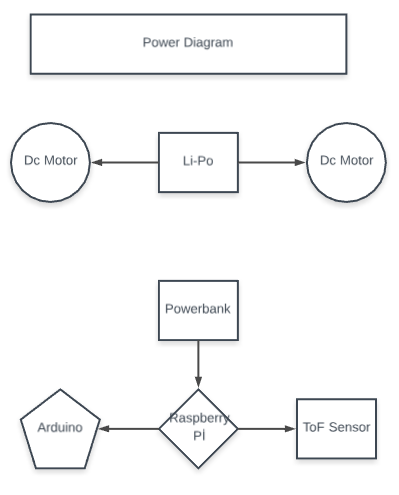
\includegraphics[width=0.5\textwidth,center]{images/elec_arch}
		\caption{Electrical Architecture of the Project}\label{fig:elec}
	\end{figure}
		
		\newpage
	
	\section{Conclusion}
	
	\newpage
		\section{Disclaimer}
		\vspace{1cm}
		
		\textsf{ All information and content contained in this report are provided solely for proof-of-concept. DUAYENLER Ltd. Şti. guarantees that the report and information contained obeys the restrictions and rules ordered by the Standard Commitee.}
		
		\vspace{1cm}
		
		
		\begin{minipage}[b]{0.33\linewidth}
			\centering
			\underline{Halil TEMURTAŞ}
		\end{minipage}%
		\begin{minipage}[b]{0.33\linewidth}
			\centering
			\underline{Erdem TUNA}
		\end{minipage}%
		\begin{minipage}[b]{0.33\linewidth}
			\centering
			\underline{Enes TAŞTAN}
		\end{minipage} \\[2.5cm]
		
		\begin{minipage}[b]{0.495\linewidth}
			\centering
			\underline{Sarper SERTEL}
		\end{minipage}%
		\begin{minipage}[b]{0.495\linewidth}
			\centering
			\underline{İlker SAĞLIK}
		\end{minipage}\\[2.5cm]
		
		\begin{minipage}[b]{0.745\linewidth}
			\centering
			~~
		\end{minipage}%
		\begin{minipage}[b]{0.25\linewidth}
			\centering
			\underline{08 March 2018}
		\end{minipage}

\newpage

\begin{appendices}
	
		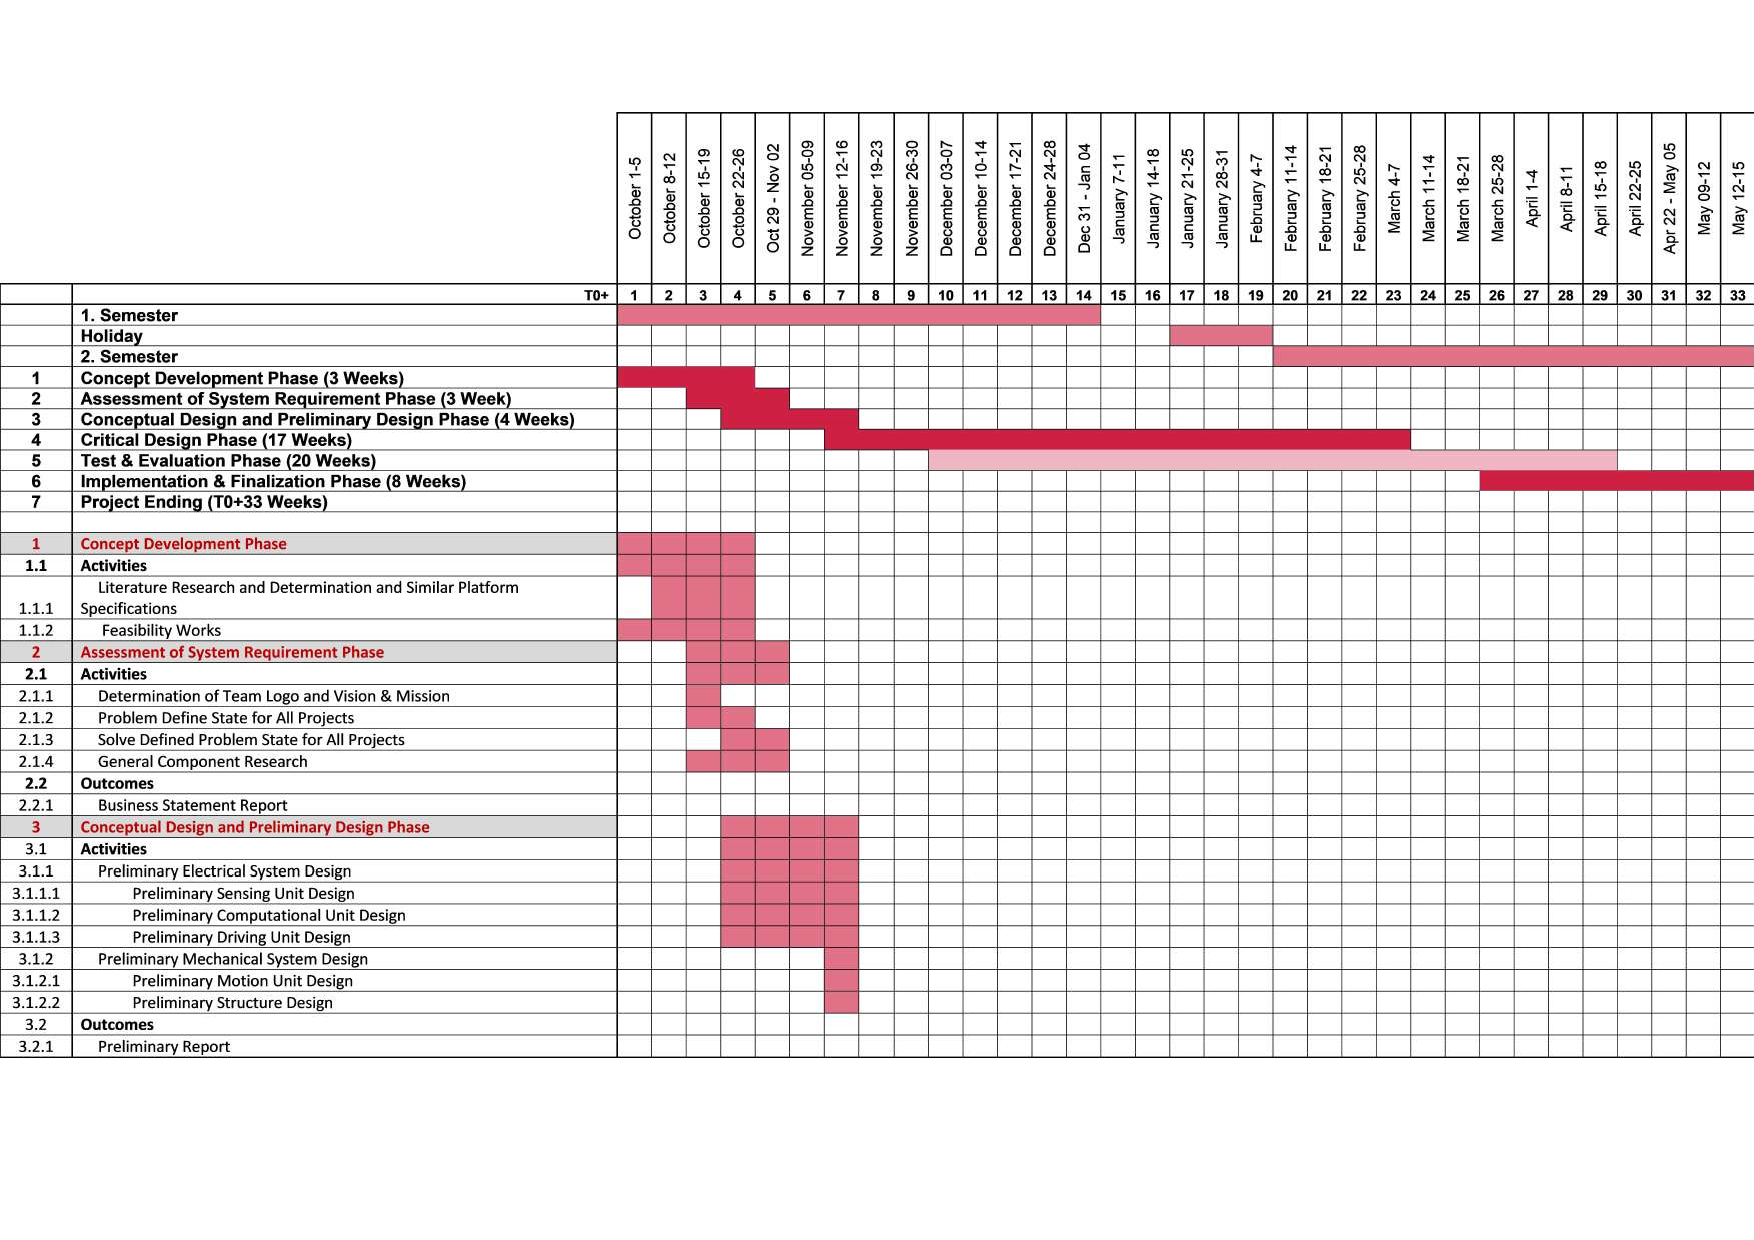
\includepdf[landscape=true,pages=1, scale=0.775,angle=0, label=gannt_chart_app,pagecommand=\section{Gannt Chart}\label{gannt_chart_app}]{gantt.pdf}
		\includepdf[landscape=true,pages=2-3, scale=0.775,angle=0,pagecommand=]{gantt.pdf}

	
\end{appendices}




	
	
	
\end{document}

%----samples------
%\begin{itemize}
%\item Item
%\item Item
%\end{itemize}

%\begin{figure}[H]
%\center
%\setlength{\unitlength}{\textwidth} 
%
\includegraphics[width=0.7\unitlength]{images/logo1}
%\caption{\label{fig:logo}Logo }
%\end{figure}

%\begin{figure}[H]
%	\setlength{\unitlength}{\textwidth} 
%	\centering
%	\begin{subfigure}{.5\textwidth}
%  		\centering
%  		
\includegraphics[width=0.48\unitlength]{images/logo1}
%  		\caption{\label{fig:logo1}Logo1 }
%	\end{subfigure}%
%	\begin{subfigure}{.5\textwidth}
%  		\centering
%		
\includegraphics[width=0.48\unitlength]{images/logo2}
%  		\caption{\label{fig:logo2}Logo2}
%	\end{subfigure}
%\caption{\label{fig:calisandegree} Small Logos   }
%\end{figure}

%\begin{table}[H]
%  \centering
% 
%    \begin{tabular}{c|c|c}
%       $$A$$ & $$B$$ & $$C$$ \\ \hline
%       1 & 2 & 3  \\ \hline
%       2 & 3 & 4  \\ \hline
%       3 & 4 & 5  \\ \hline
%       4 & 5 & 6  
%      
%  \end{tabular}
%  \caption{table}
%  \label{tab:table}
%\end{table}

%\begin{table}[H]
%  \centering
% 
%    \begin{tabular}{c|c|c}
%       \backslashbox{$A$}{$a$} & $$\specialcell{ Average deviation \\ after subtracting out the  \\ frequency error }$$ & $$C$$ \\ \hline
%       \multirow{2}{*}{1} & 2 & 3  \\ \cline{2-3}
%        & 3 & 4  \\ \hline
%       3 & \multicolumn{2}{c}{4}  \\ \hline
%       4 & 5 & 6  
%      
%  \end{tabular}
%  \caption{table}
%  \label{tab:table}
%\end{table}
%-----end of samples-----